% LaTeX source for ``Algorithms for Computer Simulation of Molecular Systems''
% Copyright (c) 2023 รังสิมันต์ เกษแก้ว (Rangsiman Ketkaew).

% License: Creative Commons Attribution-NonCommercial-NoDerivatives 4.0 International (CC BY-NC-ND 4.0)
% https://creativecommons.org/licenses/by-nc-nd/4.0/

\chapter{กลศาสตร์ควอนตัมเชิงโมเลกุล}
\label{ch:mol_qm}

%----------------------------------------
\section{การจำลองเชิงตัวเลขและเทคนิคเชิงคอมพิวเตอร์}
%----------------------------------------

การจำลองเชิงตัวเลข (Numerical Modeling) คือวิธีการที่เราใช้แก้ปัญหาทางคณิตศาสตร์และฟิสิกส์แบบต่าง ๆ เช่น นำมาใช้แก้สมการเชิงอนุพันธ์
(Differential Equations) ที่ใช้ในการอธิบายปรากฏการณ์ต่าง ๆ ทางธรรมชาติซึ่งอาจจะมีความยากหรืออาจจะไม่มีทางแก้ได้ด้วยวิธีเชิงวิเคราะห์
(Analytical Method)
\idxboth{การจำลองเชิงตัวเลข}{Numerical Modeling}
\idxboth{วิธีเชิงวิเคราะห์}{Analytical Method}

สำหรับการจำลองด้วยเทคนิคเชิงคอมพิวเตอร์ (Computer Simulation) นั้นเป็นการศึกษาการตอบสนองเชิงพลวัต (Dynamic Response)
ของระบบที่เราศึกษาและจำลองภายใต้เงื่อนไขเริ่มต้น (Initial Conditions) ที่เราได้กำหนดไว้ โดยเงื่อนไขเริ่มต้นนี้สอดคล้องกับสภาวะจริงของระบบนั้น
\idxboth{เทคนิคเชิงคอมพิวเตอร์}{Computer Simulation}
\idxboth{เงื่อนไขเริ่มต้น}{Initial Conditions}

\begin{figure}[htbp]
  \centering
  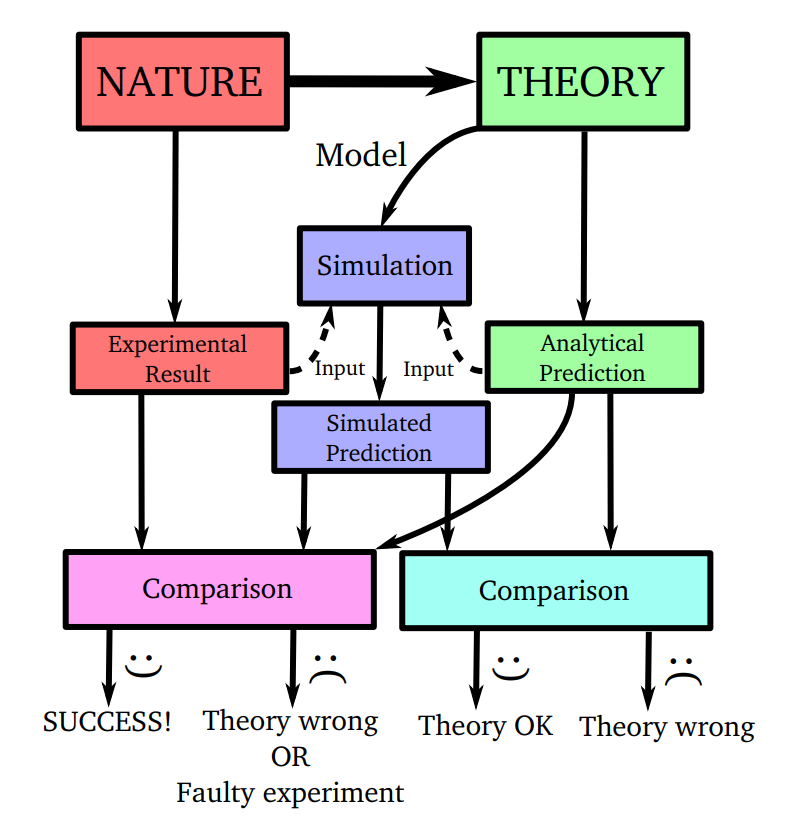
\includegraphics[width=0.8\linewidth]{fig/simulation-modeling-graph.png}
  \caption{แผนผังความเชื่อมโยงของระบบที่เราต้องศึกษา (Nature), ทฤษฎีหรือวิธีที่ใช้ในการศึกษา (Theory), แบบจำลองหรือโมเดล
    (Model), ผลการทดลอง (Experimental Result), และผลการคำนวณหรือผลการทำนาย (Computational Results หรือ Prediction)}
  \label{fig:sim_model_graph}
\end{figure}

ภาพที่ \ref{fig:sim_model_graph} แสดงแผนผังเชื่อมโยงความแตกต่างระหว่าง Numerical Modeling กับ Computer Simulation
นั้นก็คือใน Simulation นั้นระบบจำลองของเราจะถูกสร้างขึ้นมา เช่น เราสร้างระบบที่เป็นโมเลกุลน้ำหลาย ๆ โมเลกุลเกาะกลุ่มรวมกัน (Water
Cluster) โดยเราหวังว่า Water Cluster ที่เราสร้างขึ้นมานี้จะสามารถเป็นตัวแทนของระบบของโมเลกุลน้ำจริง ๆ ได้ ซึ่งก็จะทำให้เราสามารถ%
ศึกษาคุณสมบัติต่าง ๆ ของโมเลกุลน้ำได้ตามต้องการ ส่วนการจำลองเชิงตัวหรือ Numerical Simulation นั้นจะเป็นการสร้างการทดลองเสมือนจริง
(Virtual Experiments) ของระบบจำลองขึ้นมา อย่างไรก็ตามในบทความวิชาการทางด้านเคมีเชิงคำนวณหรือชีวเชิงคำนวณนั้นเรามักจะพบว่าคำว่า
Modeling นั้นสามารถถูกแทนด้วยคำว่า Simulation ได้เช่นกัน

คำถามสำคัญที่หลายคนโดยเฉพาะอย่างนักวิทยาศาสตร์ที่ทำงานวิจัยเชิงการทดลองมักจะถามก็คือ \enquote{ทำไมการจำลองทางคอมพิวเตอร์ถึงมีความสำคัญ?}
ซึ่งคำตอบนั้นมีด้วยกันหลายข้อ โดยผมขอสรุปเป็นประเด็นตามนี้

\begin{enumerate}[topsep=0pt,noitemsep]
  \setlength\itemsep{1em}
  \item การจำลองทางคอมพิวเตอร์นั้นเปรียบเสมือนเป็นสะพานเชื่อมโยงระหว่างทฤษฎีกับการทดลอง

  \item การทำการทดลองบางอย่างนั้นมีค่าใช้จ่ายที่สูงมากและมีความยากเพราะว่าตัวทฤษฎีนั้นซับซ้อนเกินไป ดังนั้นการจำลองทางคอมพิวเตอร์%
        นั้นจะเข้ามาช่วยในการจำลองการทดลองและทดสอบสมมติฐานเพื่อยืนยันทฤษฎีด้วย

  \item การจำลองทางคอมพิวเตอร์นั้นช่วยหาปัจจัยและเงื่อนไขที่เหมาะสมสำหรับการทดลองได้

  \item การจำลองทางคอมพิวเตอร์สามารถแสดงกระบวนการของระบบที่เราสนใจได้ ซึ่งอาจจะทำได้ยากในเชิงการทดลอง

  \item การจำลองทางคอมพิวเตอร์สามารถนำมาใช้ในการศึกษาปรากฏการณ์ที่การทดลองนั้นอาจจะให้ผลการทดลองที่ไม่ละเอียดพอ
\end{enumerate}

อย่างไรก็ตามผมต้องขอสรุปเพิ่มเติมด้วยว่าการใช้แบบจำลองทางคอมพิวเตอร์เพียงอย่างเดียวนั้นจะเปล่าประโยชน์ถ้าหากว่าไม่มีผลการทดลองที่%
น่าเชื่อมายืนยันความถูกต้องของผลการคำนวณ ดังนั้นเคมีเชิงการทดลองกับเคมีเชิงคำนวณนั้นจึงเป็นศาสตร์ที่ต้องพึ่งพาอาศัยกัน

%----------------------------------------
\section{พื้นฐานคณิตศาสตร์ที่ต้องรู้}
%----------------------------------------

%----------------------------------------
\subsection{ทำไมคณิตศาสตร์จึงสำคัญต่อการเรียนเคมีควอนตัม}
%----------------------------------------

\enquote{พื้นฐานอะไรที่สำคัญที่สุดในการเริ่มศึกษาและทำวิจัยด้านกลศาสตร์เคมีควอนตัม?} คำถามนี้เป็นคำถามง่าย ๆ แต่ว่าหลายคนนั้นมองข้ามไป
ผมเริ่มต้นด้วยคำถามนี้ก็เพราะว่าอยากให้ผู้อ่านนั้นตระหนักก่อนว่าเนื้อหาของวิชากลศาสตร์ควอนตัมโดยเฉพาะเคมีควอนตัมนั้นมีความยากและซับซ้อนมาก ๆ
ซึ่งในการเริ่มศึกษานั้น นอกจากความรู้เคมีที่เราจะต้องมีแล้ว เราจะต้องมีความรู้ทางคณิตศาสตร์ด้วย เพราะว่าในกลศาสตร์ควอนตัมเกี่ยวข้องกับสมการต่าง ๆ
มากมาย มีทั้งการพิสูจน์ การดำเนินการต่าง ๆ และรวมถึงการคำนวณที่ซับซ้อน

คำถามถัดมาคือ \enquote{แล้วหัวข้อไหนในคณิตศาสตร์ที่สำคัญและจำเป็นที่สุดสำหรับการศึกษากลศาสตร์ควอนตัมล่ะ?} ในการตอบคำถามนี้
ผู้อ่านต้องเข้าใจก่อนว่าในเคมีควอนตัมนั้นใช้คณิตศาสตร์หลายหัวข้อมาก ๆ ในการพิสูจน์และแก้สมการต่าง ๆ ซึ่งมีความจำเป็นและจะมองข้ามไปไม่ได้เลย
เท่าที่ผมไปอ่านโพสต์ในฟอรั่มของต่างประเทศที่ได้พูดคุยกันเกี่ยวกับสกิลพื้นฐานที่จำเป็นสำหรับการเรียนเคมีควอนตัมมานั้น ผมจับใจความและขอสรุปดังนี้
(เป็นพื้นฐานที่จำเป็นสำหรับการศึกษาควอนตัมทุกแขนง ไม่เพียงแค่เคมีควอนตัมเท่านั้น)

\begin{enumerate}[topsep=0pt,noitemsep]
  \setlength\itemsep{1em}
  \item Linear Algebra : อย่างน้อย ๆ เลยสิ่งที่ต้องรู้นั่นก็คือพื้นฐานเรื่องเมทริกซ์ (Matrix), ปริภูมิเวกเตอร์ (Vector Spaces),
        Eigenvalues, Eigenvectors นั่นก็เพราะว่ากลศาสตร์ควอนตัมนั้นเกี่ยวข้องกับเวกเตอร์ ส่วนความรู้ Eigenvalues กับ Eigenvectors
        นั้นเราจะใช้ในการแก้สมการชโรดิงเงอร์สำหรับ Stationary State ของอะตอมหรือโมเลกุล

  \item Calculus: Derivatives, Integrals, Taylor Expansions เราใช้แคลคูลัสเยอะมากในการดำเนินการหรือตรวจสอบคุณสมบัติ%
        ของฟังก์ชันคลื่น รวมถึงเงื่อนไขขอบเขต (Boundary Condition) ต่าง ๆ

  \item Differential Equations และ Partial Differential Equations ใช้ในการแก้สมการอนุพันธ์ทั้งแบบเชิงเส้นและไม่เชิงเส้น

  \item ความรู้ด้านพิกัดระบบต่าง ๆ เช่น Cartesian Coordinates, Cylindrical Coordinates และ Spherical Coordinates
        ซึ่งระบบพิกัดต่าง ๆ นี้ก็จำเป็นสำหรับการศึกษาอนุภาค

  \item พื้นฐานเรื่องความน่าจะเป็น (Probability) : ความน่าจะเป็นนั้นใช้เยอะมากในกลศาสตร์ควอนตัมเชิงสถิติ (Statistical Quantum
        Mechanics) รวมไปถึงการนำกลศาสตร์ไปอธิบายกับทฤษฎีหรือปรากฏการณ์ต่าง ๆ

  \item หัวข้ออื่น ๆ : นอกจากนี้ยังมีหัวข้ออื่น ๆ อีกที่จำเป็นต้องรู้สำหรับการศึกษากลศาสตร์ควอนตัมขั้นสูง เช่น Relativistic Quantum
        Mechanics
        \begin{enumerate}[noitemsep]
          \setlength\itemsep{0.5em}
          \item Complex Analysis (โดยเฉพาะ Complex Integration)

          \item Functional Integration

          \item Functional Analysis

          \item Group Theory

          \item Calculus of Variations หรือ Variational Calculus

          \item Functional Integration

          \item Tensor Calculus
        \end{enumerate}
\end{enumerate}

%----------------------------------------
\subsection{ทุกอย่างเกี่ยวข้องกับเวกเตอร์และเมทริกซ์}
%----------------------------------------

ถ้าต้องให้ผมเลือกหนึ่งหัวข้อที่คิดว่าสำคัญมาก ๆ ทั้งในแง่การนำมาใช้ในการพัฒนาทฤษฎีรวมถึงการนำไปประยุกต์ใช้งานจริง ผมคิดว่าพีชคณิตเชิงเส้น
(Linear Algebra) โดยเฉพาะเรื่องเวกเตอร์และเมทริกซ์นั้นน่าจะสำคัญมากที่สุด เหตุผลก็คือผมคิดว่าเมทริกซ์นั้นเป็นพื้นฐานมากที่สุดในกลศาสตร์ควอนตัม
เริ่มตั้งแต่การกำหนดหรือนิยามตัวแปรและพารามิเตอร์ต่าง ๆ เลยก็ว่าได้ ซึ่งเราใช้เวกเตอร์หรือเมทริกซ์ทั้งนั้น นอกจากนี้ในกลศาสตร์ควอนตัมนั้นเรามัก%
จะวนเวียนและวุ่นวายอยู่กับฟังก์ชันคลื่น (Wavefunction) เริ่มตั้งแต่การ Represent ฟังก์ชันคลื่นเราก็ใช้เวกเตอร์และเมทริกซ์, การดำเนินการ
(Operation) ต่าง ๆ ก็ใช้เอกลักษณ์และคุณสมบัติของเมทริกซ์ ดังนั้นความรู้เกี่ยวกับเมทริกซ์นั้นจึงเป็นสิ่งที่เราจำเป็นต้องใช้และไม่มีใครหนีพ้น
ซึ่งนี่ยังไม่รวมถึงการนำไปใช้งานจริงในกลศาสตร์ควอนตัมเชิงการคำนวณ (Computational Quantum Mechanics) ซึ่งเกี่ยวข้องกับการเขียน%
โปรแกรมที่เราจำเป็นที่จะต้องแก้สมการเชิงเส้นต่าง ๆ เพื่อหาคำตอบออกมา

ตัวอย่างอันหนึ่งที่เห็นภาพได้ชัดก็คือสมการชโรดิงเงอร์ (ผมจะยังไม่ลงรายละเอียด ณ ตอนนี้)

\begin{tcolorbox}[ams equation]
  \texttt{Hamiltonian} \cdot \texttt{Wavefunction}
  =
  \texttt{Energy} \cdot \texttt{Wavefunction}
\end{tcolorbox}

\noindent จะเห็นได้ว่าเรามีทั้ง Hamiltonian, Wavefunction, และ Energy อยู่ในสมการ ซึ่งทั้ง 3 พารามิเตอร์นี้นั้นในสามารถถูกเขียนได้ง่าย ๆ
เลยด้วยการใช้เมทริกซ์ซึ่งทำให้ง่ายต่อการตีความ เมื่อตัวแปรทั้ง 3 ตัวเป็นแค่เมทริกซ์ เวลาที่เราจะเขียนฟังก์ชันคลื่นให้อยู่ในรูปการกระจายในฟอร์มต่าง ๆ
แบบไหนก็ตามก็ทำได้ง่ายขึ้น นอกจากนี้เรายังสามารถใช้คุณสมบัติของเมทริกซ์เข้ามาช่วยได้อีก เช่น สำหรับวิชาโครงสร้างเชิงอิเล็กทรอนิกส์ (Electronic
Structure) ซึ่งเป็นหัวข้อหนึ่งของเคมีควอนตัมนั้น เราสามารถเขียนฟังก์ชันคลื่นให้อยู่ในรูปของผลรวมเชิงเส้นของผลคูณระหว่าง Basis Function
กับสัมประสิทธิ์ออร์บิทัลเชิงโมเลกุล (Molecular Orbitals Coefficient) ได้

นอกจากนี้แล้ว การที่เราเข้าใจเรื่องเมทริกซ์นั้นยังช่วยให้เราเข้าใจวิธีหรือกระบวนการในการแก้สมการต่าง ๆ ในกลศาสตร์ควอนตัมอย่างเป็นขั้นเป็นตอน
โดยเฉพาะตอนที่เราจะต้องเขียนโปรแกรมเพื่อแก้สมการนั้น เราก็ใช้เมทริกซ์เยอะมาก ๆ

%----------------------------------------
\subsection{เบซิส}
%----------------------------------------

สิ่งแรกที่ต้องทำความเข้าใจเกี่ยวกับตัวแปรทางเคมีควอนตัมก็คือปริภูมิของเวกเตอร์ (Vector) โดยเราเริ่มต้นด้วยการใช้ Dirac Notation
สำหรับ Vector Space $S$ นั้น เรากำหนดให้ $\alpha \ket{a}$ เป็นสมาชิกของ $S$ และเราทำการกำหนดสิ่งที่เรียกว่า \textbf{Dual
  Vector} $\alpha^* \bra{a}$ โดยที่ $\alpha^*$ นั้นเป็น Complex Conjugate ของ $\alpha$

สำหรับการดำเนินการทางคณิตศาสตร์ของเวกเตอร์อันแรกที่เราควรจะต้องรู้นั้นก็คือการคูณแบบภายของเวกเตอร์ 2 อัน \textbf{Inner Product}
(เช่น $\ket{a}$ กับ $\ket{b}$) ซึ่งจะได้ผลลัพธ์เป็นตัวเลขหรือปริมาณสเกลาร์ ดังนี้

\begin{equation}
  \braket{a}{b}
  =
  \alpha \in \mathbb{C}
\end{equation}

\noindent ซึ่งการคูณแบบนี้เป็นการคูณแบบจุดของระหว่างเวกเตอร์นั่นเอง $(\bm{u} \cdot \bm{v})$ และการนิยามการคูณแบบนี้%
จะทำให้การสลับที่ของเวกเตอร์นั้นยังคงให้ Complex Conjugate ที่เหมือนกันอยู่

\begin{equation}
  \label{eq:braket_conjugate}
  \braket{b}{a}
  =
  \braket{a}{b}^*
  = \alpha^*
\end{equation}

\noindent โดยเราเรียกเวกเตอร์ $\ket{a}$ กับ $\ket{b}$ ที่มีผลลัพธ์เป็น 0 (Zero Inner Product) หรือ $ \braket{a}{b} = 0$
ว่าเป็น \textbf{Orthogonal} นอกจากนี้ Inner Product ของทั้งสองเวกเตอร์นั้นยังมีความเป็นเส้นตรงหรือ \textbf{Linear} อีกด้วย ดังนี้

\begin{equation}
  \braket{c}{\alpha a + \beta b}
  =
  \alpha \braket{c}{a} + \beta \braket{c}{b}
\end{equation}

\noindent และมีความเป็น \textbf{Anti-Linear}\footnote{ผมไม่รู้ว่าจะแปลคำว่า Anti-Linear ยังไงดี} ดังนี้

\begin{equation}
  \braket{\alpha a + \beta b}{c}
  =
  \alpha^* \braket{a}{c} + \beta^* \braket{b}{c}
\end{equation}

นอกจากนี้ยังเราสามารถนิยาม Norm ของเวกเตอร์ได้ด้วย (โดยที่เรายังใช้ Notation ของ Inner Product อยู่) ดังนี้

\begin{equation}
  \| \ket{a} \|
  =
  \sqrt{\braket{a}{a}} \in \mathbb{R}
\end{equation}

\noindent ซึ่ง Norm ตามที่นิยามนี้มีเงื่อนไขดังต่อไปนี้

\begin{equation}
  \begin{split}
    \| \ket{a} \| > 0 \text{ if } \ket{a} \neq \ket{0} \\
    \| \ket{a} \| = 0 \text{ if } \ket{a} = \ket{0}
  \end{split}
\end{equation}

\noindent และเราก็เรียกเวกเตอร์ $\ket{a}$ ที่มี Unit Norm ($\braket{a}{a} = 0$) ว่าเป็น \textbf{Normalized Vector}
หรือเวกเตอร์ที่ถูกทำให้เป็นปกติ

ลำดับถัดมาที่ผมอยากจะให้ผู้อ่านทำความเข้าใจก็คือการ Represent ปริภูมิเวกเตอร์ในทางกลศาสตร์ควอนตัม ต้องเกริ่นก่อนว่าปริภูมิเวกเตอร์ $S$
นั้นจริง ๆ แล้วก็เป็นแค่เซตของเวกเตอร์หลาย ๆ อันนั่นเอง (เราเลยเรียกว่าปริภูมิ) ซึ่งถ้าหากว่าเซตของเวกเตอร์ของเรานั้นมีหลาย ๆ เวกเตอร์
ก็จะทำให้ปริภูมิเวกเตอร์ของเรานั้นมีจำนวนมิติที่มากตามไปด้วย โดยจำนวนมิติของปริภูมิเวกเตอร์นั้นก็จะเท่ากับจำนวนของเวกเตอร์ $(N)$
ดังนั้นเราจึงเขียน \textbf{เบซิส} เป็นภาษาทางคณิตศาสตร์ได้ดังนี้ $\{ \ket{\phi_i}, i = 1,\ldots,N \}$ โดยที่เราสามารถเขียนเวกเตอร์
$\ket{a} \in S$ ได้ในรูปของผลรวมเชิงเส้นของสมาชิกแต่ละตัวในเบซิส (ซึ่งสมาชิกแต่ละตัวก็คือเวกเตอร์นั่นเอง)

\begin{tcolorbox}[ams equation]
  \label{eq:basis}
  \ket{a} = \sum_{i = 1}^N a_i \ket{\phi_i}
\end{tcolorbox}

\noindent โดยที่ $a_i$ นั้นคือค่าสัมประสิทธิ์ของสมาชิกของเบซิสแต่ละตัวซึ่งจะมีค่าจำเพาะและไม่เหมือนกัน ผมอยากให้ลองคิดตามง่าย ๆ ว่า
\textit{จริง ๆ แล้ว $\ket{a}$ นั้นก็เป็นแค่ผลลัพธ์ที่ได้จากการคูณแบบจุด (Dot Product) ของเวกเตอร์แบบแถวของฟังก์ชันเบซิส
  $\ket{\boldsymbol \phi} = (\ket{\phi_1}, \ket{\phi_2}, \ldots, \ket{\phi_N})$ กับเวกเตอร์แบบหลักของสัมประสิทธิ์
  $\bm{a}  = (a_1,a_2,\ldots,a_N)^T$}

\begin{equation}
  \label{eq:basis_dual_vector}
  \ket{a}
  =
  (\ket{\phi_1}, \ket{\phi_2}, \ldots, \ket{\phi_N})
  \begin{pmatrix}
    a_1    \\
    a_2    \\
    \vdots \\
    a_N
  \end{pmatrix}
  = \ket{\boldsymbol \phi} \bm{a}
\end{equation}

\noindent โดยที่ $\bra{\boldsymbol \phi}$ คือเวกเตอร์แบบหลักของ Dual Vector ซึ่งมีหน้าตาดังต่อไปนี้

\begin{equation}
  \bra{\boldsymbol \phi}
  =
  \begin{pmatrix}
    \bra{\phi_1} \\
    \bra{\phi_2} \\
    \vdots       \\
    \bra{\phi_N}
  \end{pmatrix}
\end{equation}

ปริมาณอีกอันหนึ่งที่สำคัญมาก ๆ ในเคมีควอนตัมเพราะเป็นปริมาณที่สามารถบ่งบอกได้ถึงคุณลักษณะของเบซิสนั่นก็คือเมทริกซ์ซ้อนทับ (Overlap Matrix)
ซึ่งมีนิยามดังนี้

\begin{tcolorbox}[ams equation]
  S_{ij}
  =
  \braket{\phi_i}{\phi_j}
\end{tcolorbox}

\noindent และเมื่อผู้อ่านศึกษาเคมีควอนตัมไปเรื่อย ๆ จะพบว่าบ่อยครั้งที่เราจะต้องเจอกับสิ่งที่เรียกว่า \textbf{Orthonormal Bases}
ซึ่งก็คือเบซิส พูดง่าย ๆ คือ Orthonormal Basis นั้นก็คือเบซิสที่มีคุณสมบัติ Orthogonal และ Normal ผสมกันอยู่นั่นเอง

\begin{equation}
  \begin{split}
    \braket{\phi_i}{\phi_i} &= 1 \quad \forall i \\
    \braket{\phi_i}{\phi_j} &= 0 \quad \forall ij, i \neq j
  \end{split}
\end{equation}

\noindent แต่เรามักจะพบเห็นการเขียนเขียนเงื่อนไขของ Orthonormality ตามตำราหรือบทความงานวิจัยที่สั้นและกระชับกว่า ดังนี้

\begin{tcolorbox}[ams equation]
  \braket{\phi_i}{\phi_j}
  =
  \delta_{ij} \quad \forall ij
\end{tcolorbox}

\noindent โดยที่ $\delta_{ij}$ นั้นมีชื่อเรียกว่า Kronecker Delta Function

เรายังสามารถที่จะเขียน Overlap Matrix ได้โดยการใช้ Expression ดังต่อไปนี้

\begin{align}
  \bm{S}
   & =
  \braket{\boldsymbol \phi}{\boldsymbol \phi }       \\
   & =
  \begin{pmatrix}
    \bra{\phi_1} \\
    \bra{\phi_2} \\
    \vdots       \\
    \bra{\phi_N}
  \end{pmatrix}
  (\ket{\phi_1}, \ket{\phi_2}, \ldots, \ket{\phi_N}) \\
   & =
  \begin{pmatrix}
    \braket{\phi_1}{\phi_1} & \braket{\phi_1}{\phi_2} & \cdots & \braket{\phi_1}{\phi_N} \\
    \braket{\phi_2}{\phi_1} & \braket{\phi_2}{\phi_2} & \cdots & \braket{\phi_2}{\phi_N} \\
    \vdots                  &                         & \ddots & \vdots                  \\
    \braket{\phi_N}{\phi_1} & \braket{\phi_N}{\phi_2} & \cdots & \braket{\phi_N}{\phi_N}
  \end{pmatrix}
\end{align}

จากข้อมูลที่เรามีเกี่ยวกับ Overlap Matrix ถ้าหากว่าเรามี \textbf{Orthonormal Basis} เราจะสามารถหาค่าของสัมประสิทธิ์ตามสมการ
\eqref{eq:basis} ได้โดยการใช้ Inner Product ของ $\ket{a}$ กับสมาชิกแต่ละตัวของเบซิส

\begin{align}
  \label{eq:basis2}
  \braket{\phi_k}{a}
   & =
  \sum_{i = 1}^N a_i \braket{\phi_k}{\phi_i}                                             \\
   & =
  \sum_{i = 1}^N a_i \delta_{ki}                                                         \\
   & =
  a_1 \delta_{k1} + a_2 \delta_{k2} + \ldots + a_k \underbrace{\delta_{kk}}_{1} + \ldots \\
   & = a_k
\end{align}

\noindent จะเห็นได้ว่าสมการด้านบนนั้นถูกลดรูปจากอนุกรมเหลือแค่ $a_k$ ซึ่งถ้าสังเกตให้ดีจะพบว่าทริคที่เราใช้ในการ Simplify สมการชุดนี้ก็%
คือว่าจะมีแค่เทอมที่ Index $i$ มีค่าเท่ากับ $k$ เท่านั้นที่จะมีค่าเท่ากับ 1 (ตามเงื่อนไข Kronecker Delta Function ก่อนหน้านี้) ซึ่งการทำ
Simplication แบบนี้เป็นเทคนิคอย่างหนึ่งที่ผู้อ่านควรจะต้องทำความคุ้นเคยให้ดี เพราะว่าเราจะใช้ทริคนี้อีกเยอะเลยในเคมีควอนตัม
สรุปคือสมการ \eqref{eq:basis2} นั้นแสดงให้เราเห็นว่าสัมประสิทธิ์ $a_k$ นั้นเป็น Inner Product $\braket{\phi_k}{a}$
ในการกระจายของเวกเตอร์ $\ket{a}$

ถ้าหากว่าเรามีเวกเตอร์ 2 อัน เช่น $\ket{a}$ กับ $\ket{b}$ ที่ถูกเขียนให้กระจายในรูปของ Orthonormal Basis ที่เหมือนกัน ดังนี้

\begin{equation}
  \begin{split}
    \ket{a} &= \sum_{i = 1}^N a_i \ket{\phi_i} \\
    \ket{b} &= \sum_{i = 1}^N b_i \ket{\phi_i}
  \end{split}
\end{equation}

\noindent เราจะสามารถเขียน Inner Product ของเวกเตอร์ทั้ง 2 อันนี้ได้ตามนี้

\begin{equation}
  \begin{split}
    \braket{a}{b} &= \braket{\sum_{i = 1}^N a_i \phi_i}{\sum_{j = 1}^N b_j \phi_j }
    = \sum_{i = 1}^N  \sum_{j = 1}^N a_i^*  \underbrace{\braket{\phi_i}{\phi_j}}_{\delta_{ij}} b_j \\
    &= \sum_{i = 1}^N a_i^* b_i = (\alpha^*_1, \alpha^*_2,\ldots)
    \begin{pmatrix}
      b_1 \\
      b_2 \\
      \vdots
    \end{pmatrix} =
    \bm{a}^\dagger\bm{b}
  \end{split}
\end{equation}

\noindent โดยเทอมขวาสุดของสมการนี้เป็นการเขียน Inner Product ในเทอมของ Dot Product ระหว่างเวกเตอร์ ($\bm{a}^\dagger
\bm{b}$) แล้วก็ตัวห้อย ``${}^\dagger$'' นั้นคือ \textbf{Conjugate Transpose ของเวกเตอร์}\footnote{เราสามารถคำนวณ 
Conjugate Tranpose ได้โดยการนำเมทริกซ์มาทำการ Tranpose แล้วคำนวณ Complex Conjugate ของสมาชิกแต่ละตัว} 
ซึ่งนี่แสดงให้เห็นว่าในการหา Orthonormal Basis นั้น เราสามารถเขียนกระจาย Inner Product ของเวกเตอร์ 2 อันได้โดยการใช้ Inner 
Product ของสัมประสิทธิ์ของเวกเตอร์

%----------------------------------------
\subsection{ตัวดำเนินการเชิงเส้น}
%----------------------------------------

\enquote{ตัวดำเนินการ (Operators) คืออะไร?} ในหัวนี้เราจะมาหาคำตอบกันครับ ผมคิดว่านิยามอย่างเป็นทางการของ \enquote{ตัวดำเนินการ} 
ที่พอจะเข้าใจได้ง่ายหน่อยนั่นก็คือ \enquote{วัตถุทางคณิตศาสตร์} (Mathematical Objects) แบบหนึ่งที่สามารถแปลงเวกเตอร์อันหนึ่งไปเป็น%
เวกเตอร์อีกอันหนึ่งได้ (เปลี่ยนเวกเตอร์อันเก่าให้เป็นอันใหม่)

\begin{equation}
  \label{eq:operator}
  \hat{A} \ket{a}
  =
  \ket{b}
\end{equation}

\noindent สำหรับเคมีควอนตัมนั้นเราจะสนใจเฉพาะ \textbf{ตัวดำเนินการเชิงเส้น} (Linear Operators) เป็นพิเศษ ซึ่งจะต้องสอดคล้องกับ%
เงื่อนดังต่อไปนี้ด้วย

\begin{equation}
  \hat{A} (\alpha \ket{a} + \beta \ket{b})
  =
  \alpha \hat{A} \ket{a} + \beta \hat{A} \ket{b}
\end{equation}

นอกจากนี้แล้วยังมีเรื่องของการกระทำ (Action) ของตัวดำเนินการต่อเวกเตอร์อีกด้วย โดยเราจะใช้สิ่งที่เรียกว่า \textbf{Matrix Representation}
ซึ่งผมอยากจะให้ผู้อ่านลองดูสมการด้านล่างต่อไปนี้ก่อน

\begin{equation}
  \begin{split}
    \sum_{i = 1}^N \underbrace{\bra{\phi_k}\hat{A} \ket{\phi_i}}_{A_{ki} } a_i
    &=
    \sum_i b_i \braket{\phi_k}{\phi_i} \\
    \sum_{i = 1}^N A_{ki} a_i
    &=
    b_k
  \end{split}
\end{equation}

\noindent จะเห็นได้ว่าเราสามารถทำการคำนวณ Inner Product ระหว่างเวกเตอร์และโอเปอร์เรเตอร์ $\hat{A}$ ได้ ซึ่งสิ่งที่เราได้ออกมานั้นคือ
$A_{ki}$ ซึ่งก็คือ Matrix Representation ของโอเปอร์เรเตอร์ $\hat{A}$ นั่นเอง โดย Matrix Representation อันนี้มีนิยามคือ
$A_{ki} = \bra{\phi_k}\hat{A} \ket{\phi_i}$ แล้วเรายังสามารถเขียนสมการด้านบนนี้ให้กระชับกว่านี้ได้โดยการใช้ Matrix-Vector
Notation ดังนี้

\begin{equation}
  \bm{b}
  =
  \bm{A} \bm{a}
\end{equation}

\noindent โดยที่ $\bm{A}$ คือเมทริกซ์ที่มีสมาชิกแต่ละตัวเป็น $(\bm{A})_{ki} = \bra{\phi_k}\hat{A} \ket{\phi_i}$

ลำดับถัดมาเราจะมาดูรายละเอียดว่าเราจะสามารถเขียนกระจายโอเปอร์เรเตอร์ในรูปของ Outer Product ของสมาชิกแต่ละตัวของเบซิส ซึ่ง
\textbf{Outer Product} ของเวกเตอร์ 2 อัน ($\ket{a}$ กับ $\ket{b}$) นั้นมีสมการดังต่อไปนี้

\begin{equation}
  \ket{a}\bra{b}
\end{equation}

\noindent เมื่อเรานำ Outer Product มาคูณกับ Ket Vector (โดยให้ Ket Vector นั้นอยู่ทางด้านขวา) เราจะได้ Inner Product
เกิดขึ้นมาในทางด้านซ้ายนั้นเอง เช่น

\begin{equation}
  (\ket{a}\bra{b}) \ket{c}
  =
  \ket{a} \braket{b}{c}
\end{equation}

\noindent และในทำนองเดียวกัน ถ้าหากว่าเรานำ Ket Vector ไปคูณทางด้านซ้ายของ Outer Product เราก็จะได้ Inner Product ที่คล้ายกัน
นอกจากนี้เรายังพบอีกว่าโอเปอร์เรเตอร์ $\hat{A}$ ที่เรานำไปใช้กับ State $\ket{a}$ นั้นจะให้ผลลัพธ์ที่เป็น State $\ket{b}$ ออกมานั่นเอง
กล่าวคือ $\hat{A}\ket{a} = \ket{b}$ สามารถเขียนได้ดังนี้

\begin{equation}
  \hat{A} = \ket{b}\bra{a}
\end{equation}

\noindent นั่นก็เพราะว่า

\begin{equation}
  \hat{A} \ket{a}
  =
  \ket{b} \underbrace{\braket{a}{a}}_{=1}
  =
  \ket{b}
\end{equation}

ปกติแล้วเราสามารถ Represent ตัวดำเนินการเชิงเส้นได้โดยการใช้ผลรวมของ Outer Product นำมาคูณด้วย Matrix Elements ตัวอย่างเช่น
ให้ผู้อ่านลองพิจารณา Orthonormal Basis $\{ \phi_i \}$ และผลรวมของ Outer Product ของสมาชิกของแต่ละเบซิส ($\{ \phi_i \}$)
ดังนี้

\begin{equation}
  \hat{1}
  =
  \sum_i \ket{\phi_i}\bra{\phi_i}
\end{equation}

\noindent ซึ่งเราจะได้สามารถนิยามปริมาณอันใหม่นี้ได้ว่าเป็น \textbf{ตัวดำเนินการเอกลักษณ์} (Identity Operator) และเพื่อเป็นการยืนยัน%
ว่าสมการด้านบนนั้นถูกต้อง เราสามารถทำยืนยันได้โดยการนำ $\hat{1}$ ไปกระทำกับเวกเตอร์ทั่วไป $\ket{a}$ ดังนี้

\begin{equation}
  \hat{1}\ket{a}
  =
  \sum_i \ket{\phi_i}\underbrace{\braket{\phi_i}{a}}_{a_i}
  =
  \sum_i \ket{\phi_i} a_i
  =
  \ket{a}
\end{equation}

\noindent แล้วผมก็อยากจะเน้นด้วยว่าเราจะใช้เงื่อนไข $\hat{1} = \sum_i \ket{\phi_i}\bra{\phi_i}$ ได้เฉพาะกับ Orthonormal
Basis เท่านั้น

%----------------------------------------
\subsection{ความเชื่อมโยงระหว่าง Representations ของฟังก์ชันคลื่น}
%----------------------------------------

หัวข้อย่อยถัดมาที่ผมอยากให้ผู้อ่านศึกษาก็คือ Formalism ที่เกี่ยวข้องกับกลศาสตร์ควอนตัม โดยเฉพาะ Representation ที่เรานำมาใช้ในการแสดง%
ฟังก์ชันคลื่น (Wavefunction) เพื่ออธิบายให้เห็นภาพมากขึ้น เราจะเริ่มด้วยการพิจารณาเบซิสเชิงตำแหน่ง (Position Basis) $\{ \ket{x},
-\infty < x < \infty \}$ ซึ่งเบซิสอันนี้เป็น Orthogonal ด้วย กล่าวคือ $\braket{x}{x'} = 0$ ถ้าหากว่า $x \neq x'$ 
แล้วเราจะสามารถทำการ Normalize เบซิสอันนี้ให้เป็น Delta ได้ด้วย ดังนี้

\begin{equation}
  \braket{x}{x'}
  =
  \delta(x - x')
\end{equation}

\noindent ซึ่งจะทำให้อินทิกรัลของเบซิสด้านบนนี้นั้นจะมีค่าเท่ากับ 1 ดังนี้

\begin{equation}
  \int \braket{x}{x'} dx
  =
  1
\end{equation}

ดังนั้นผมจึงอยากจะสรุปให้เข้าใจง่าย ๆ ว่าแท้จริงแล้วนั้น \textit{แล้วฟังก์ชันคลื่นในทางกลศาสตร์ควอนตัมนั้นไม่ใช่อะไรเลย แต่เป็นแค่ 
Representation ของเวกเตอร์ $\ket{\Psi}$ บนเบซิสเชิงตำแหน่ง} ดังนี้

\begin{equation}
  \Psi(x) \equiv \braket{x}{\Psi}
\end{equation}

\noindent ซึ่งเราสามารถเขียน Identity Operator ในรูปของเบซิสเชิงตำแหน่งได้ดังนี้

\begin{equation}
  \hat{1}
  =
  \int \ket{x} \bra{x} dx
\end{equation}

\noindent แล้วเราก็สามารถเขียน Inner Product $\braket{\Psi}$ ในทางกลศาสตร์ควอนตัมได้ดังนี้

\begin{align}
  \braket{\Psi}
   & =
  \bra{\Psi} \left( \int \ket{x} \bra{x} dx \right) \ket{\Psi} \\
   & =
  \int \braket{\Psi}{x} \braket{x}{\Psi} dx                    \\
   & =
  \int \Psi(x)^* \Psi(x) dx                                    \\
   & =
  \int |\Psi(x)|^2 dx
\end{align}

%----------------------------------------
\subsection{ตัวดำเนินการพิเศษ}
%----------------------------------------

ลำดับถัดมาคือเรื่องของตัวดำเนินการพิเศษแบบต่าง ๆ ที่เราจะต้องพบเจอในกลศาสตร์เคมีควอนตัม โดยตัวแรกที่จะพูดถึงนั้นก็คือเมทริกซ์พิเศษแบบหนึ่ง%
ที่เรียกว่า \textbf{คอนจูเกตเอร์มีเชียน} (Hermitian Conjugate) เริ่มต้นด้วยการกำหนดให้มีตัวดำเนินการ $\hat{A}$ แล้วเราจะทำการนิยามว่า
Hermitian Conjugate ของตัวดำเนินการนี้ก็คือ $\hat{A}^\dagger$ ซึ่งกระทำอยู่บน Dual Vector ($\hat{A} \ket{a}$) โดย
Hermitian Conjugate นั้นจะต้องสอดคล้องกับเงื่อนไขต่อไปนี้

\begin{tcolorbox}[ams equation]
  \label{eq:braAket_conjugate}
  \bra{a} \hat{A} \ket{b}
  =
  \bra{b} \hat{A}^\dagger \ket{a}^*
\end{tcolorbox}

\noindent แล้วก็คุณสมบัติที่สำคัญอย่างหนึ่งของ Hermitian Conjugate ก็คือเราสามารถสลับลำดับตำแหน่งของตัวดำเนินการ พูดง่าย ๆ คือ
Hermitian Conjugate ของเวกเตอร์ 2 อันที่คูณกันนั้นจะเท่ากับ Hermitian Conjugate ของเวกเตอร์แต่ละตัวที่สลับตำแหน่งกันแล้วมาคูณกัน
ดังนี้

\begin{equation}
  (\hat{A} \hat{B})^\dagger
  =
  \hat{B}^\dagger \hat{A}^\dagger
\end{equation}

ตัวดำเนินการพิเศษที่สำคัญมากอันหนึ่งก็คือ \textbf{ตัวดำเนินการเอร์มีเชียน} (Hermitian Operator) ซึ่งมีนิยามคือต้องเป็น Hermitian
Conjugate ที่เหมือนกันกับตัวดำเนินการอันเดิม

\begin{tcolorbox}[ams equation]
  \hat{A}^\dagger = \hat{A}
\end{tcolorbox}

\noindent และด้วยคุณสมบัติพิเศษอันนี้นี่เองที่ทำให้ Hermitian Operator นั้นถูกนำมาใช้เยอะมากในเคมีควอนตัมเพราะว่ามีค่าไอเกนแบบจริง
(Real Eigenvalues) ซึ่งเป็นผลเฉลยหรือคำตอบของสมการไอเกนเวกเตอร์ ดังนี้

\begin{equation}
  \hat{A} \ket{a} = \lambda \ket{a}
\end{equation}

ตัวดำเนินการพิเศษอีกตัวที่เราควรรู้ก็คือ \textbf{ตัวดำเนินการแบบเดี่ยว} (Unitary Operator) ซึ่งมีนิยามคือต้องเป็น Hermitian Conjugate
ที่อินเวอร์ส (Inverse) ของตัวเองนั้นต้องเท่ากับตัวดำเนินการอันเดิม

\begin{tcolorbox}[ams equation]
  \hat{A}^\dagger
  =
  \hat{A}^{-1}
\end{tcolorbox}

\noindent สำหรับ Unitary Operator นั้นเรามีเงื่อนไขเพิ่มเติมต่อไปนี้ด้วย

\begin{equation}
  \begin{split}
    \hat{A}^\dagger \hat{A} = \hat{A}^{-1} \hat{A} = 1 \\
    \hat{A} \hat{A}^\dagger = \hat{A} \hat{A}^{-1} = 1
  \end{split}
\end{equation}

\noindent นอกจากนี้แล้ว Unitary Operator นั้นยังไม่เปลี่ยนค่า Norm ของ State ที่เรานำมันไปกระทำอีกด้วย ซึ่งสามารถพิสูจน์ให้ดูได้จาก%
ตัวอย่างดังต่อไปนี้

\begin{equation}
  \hat{U} \ket{a}
  =
  \ket{b}
\end{equation}

\noindent เมื่อเรานำ Unitary Operator เข้าไปกระทำกับ State $\ket{a}$ จะพบว่าเราก็จะยังได้ค่า Norm ของ $\ket{a}$ ที่เหมือนเดิม

\begin{equation}
  \| \ket{b} \|
  =
  \sqrt{\braket{b}{b}}
  =
  \sqrt{\bra{a}\hat{U}^\dagger \hat{U} \ket{a}}
  =
  \sqrt{\bra{a} \underbrace{\hat{U}^{-1} \hat{U}}_{\hat{1}} \ket{a}}
  =
  \sqrt{\braket{a}{a}}
  =
  \| \ket{a} \|
\end{equation}

\noindent เราจึงสรุปว่าได้ Unitary Operator มีความสามารถในการรักษาค่า Norm ของ State

สุดท้ายนี้ผมขอสรุปเกี่ยวกับความสำคัญของคณิตศาสตร์ต่อเคมีควอนตัมว่า ท้ายที่สุดแล้วคณิตศาสตร์ทุกหัวข้อนั้นก็มีความสำคัญเท่ากันหมดและเป็นรากฐาน 
(Foundation) ที่สำคัญในการพัฒนาวิธีใหม่ ๆ ให้ดีกว่าวิธีเดิม ๆ แต่ว่าเราจะได้นำความรู้ของแต่ละหัวข้อมาใช้มากหรือน้อยนั้นก็ขึ้นอยู่กับหัวข้อเฉพาะ%
ทางของกลศาสตร์ที่เรานั้นสนใจหรือทำงานอยู่ แม้ว่าอาจจะมีหัวข้อหลาย ๆ อันที่เราจำเป็นต้องใช้ตลอดเวลา เช่น เมทริกซ์หรือแคลคูลัส 
แต่ถ้าหากว่าเราไม่มีความรู้ของบางหัวข้อที่เราคิดว่าจะไม่ได้ใช้ เราก็คงจะมีปัญหาแน่ ๆ เมื่อถึงเวลาที่เราจำเป็นต้องใช้ความรู้เหล่านั้น

%----------------------------------------
\section{หน่วยอะตอม}
\idxboth{หน่วยอะตอม}{Atomic Units}
%----------------------------------------

ในการศึกษาอะตอมและโมเลกุลนั้น นักเคมีเชิงทฤษฎีมักจะมีการกำหนดหน่วยขึ้นมาเพื่อให้ง่ายต่อการศึกษาคุณสมบัติต่าง ๆ ของอะตอม เช่น ตำแหน่ง,
มวล, โมเมนตัม ซึ่งหน่วยหรือ Units ที่จะช่วยให้ชีวิตของนักวิจัยที่ทำงานทางด้านนี้สะดวกมากขึ้นในการพัฒนาทฤษฎีและทำให้การคำนวณง่ายขึ้นนั้น%
ควรจะต้องทำให้ค่าของคุณสมบัติต่าง ๆ ที่ได้กล่าวมานั้นมีค่าเท่ากับหรือเข้าใกล้ 1 ให้มากที่สุด ซึ่งจะช่วยให้เราไม่ต้องไปใช้ค่าจริง ๆ ของปริมาณต่าง ๆ
ในการคำนวณ ตัวอย่างเช่น เราก็ไม่จำเป็นที่จะต้องใช้ค่ามวลจริง ๆ ของอิเล็กตรอน

หน่วยที่ถูกนำมาใช้มากที่สุดในเคมีควอนตัมนั้นก็คือหน่วยอะตอม (Atomic Units ย่อสั้น ๆ เป็น a.u.) โดย Atomic Units นี้ถูกกำหนดค่าดังนี้

\begin{align}
  \text{Electron Mass}      & = m_{e} = 1                             \\
  \text{Electron Charge}    & = e = 1                                 \\
  \text{Action}             & = \hbar = \frac{h}{2\pi} = 1            \\
  \text{Coulomb's Constant} & = k_{e} = \frac{1}{4\pi \epsilon_0} = 1
\end{align}

ตารางต่อไปนี้แสดง Conversion Factor ระหว่าง Atomic Units กัยหน่วยอื่น ๆ

\begin{table}[htbp]
  \centering
  \begin{tabular}{lll}
    \toprule
    Dimension & Symbol (Name)         & Value in Other Units                            \\
    \midrule
    Length    & $a_0$ (bohr)          & 0.52918 \AA{} = 0.52918 $10^{-10}$ m            \\
    Mass      & $m_e$                 & $9.1095 \times 10^{-31}$ Kg                     \\
    Charge    & $e$                   & $1.6022 \times 10^{-19}$ C                      \\
    Action    & $\hbar$               & $1.05457 \times 10^{-34}$ J $\cdot$ s           \\
    %Coulomb's constant & $\frac{1}{4\pi \epsilon_0}$ & $ \times 10^{-34}$ J $\cdot$ s \\
    Energy    & $E_{\rm h}$ (Hartree) & 627.51 kcal/mol                                 \\
              &                       & 27.211 eV                                       \\
              &                       & 219474.63 cm$^{-1}$                             \\
              &                       & $4.3598 \times 10^{-18}$ J                      \\
    Time      &                       & $2.41889 \times 10^{-17}$ s $\approx 1/41.3$ fs \\
    \bottomrule
  \end{tabular}
  %\caption{Remember, \emph{never} use vertical lines in tables.}
  \label{tab:atomicunits}
\end{table}

\noindent ความเร็วของแสงในหน่วย Atomic Units คือ $\alpha^{-1}\approx 137$ a.u.

%----------------------------------------
\section{สมการชโรดิงเงอร์}
\idxboth{สมการชโรดิงเงอร์}{Schr\"{o}dinger Equation}
%----------------------------------------

สมการชโรดิงเงอร์เป็นสิ่งที่ช่วยให้เราสามารถเข้าใจพฤติกรรมของโมเลกุลได้ การที่เรารู้คำตอบหรือผลเฉลยของสมการนั้นนำไปสู่การเข้าใจข้อมูลต่าง ๆ
ของโมเลกุล (พูดให้ครอบคลุมกว่านี้คือระบบแบบ Microscopic) ที่อุณหภูมิ 0 K โดยสมการชโรดิงเงอร์ที่ขึ้นกับเวลา (Time-Dependent
Schr\"{o}dinger Equation) นั้นมีหน้าตาดังนี้

\begin{equation}
  \label{eq:time_dependent_schrodinger}
  \hat{H} \Psi\left(\vec{r}_{1 \ldots N}, t\right)
  =
  \mathrm{i} \hbar
  \frac
  {
    \partial \Psi\left(\vec{r}_{1 \ldots N}, t\right)
  }
  {
    \partial t
  }
\end{equation}

\noindent โดยที่ตัวแปรในสมการมีดังนี้
\begin{itemize}[topsep=0pt,noitemsep]
  \setlength\itemsep{1em}
  \item $\hat{H}$ คือโอเปอร์เรเตอร์ของพลังงาน

  \item $\Psi$ คือฟังก์ชันคลื่นที่ขึ้นอยู่กับพิกัดหรือตำแหน่งของอนุภาค (ในที่นี้คืออิเล็กตรอน) ทั้งหมด $N$ ตัว เราจึงใช้เวกเตอร์แทน
        $\vec{r}_{1}, \vec{r}_{2}, \dots, \vec{r}_{N}$

  \item $i$ คือหน่วยจินตภาพ $(\sqrt{-1})$

  \item $\hbar$ คือค่าคงที่ของพลังค์แบบลดรูป (Reduced Planck's constant) มีค่าเท่ากับ
        \num{1.05457182e-34} \si{m^{2}.kg.s^{-1}}
\end{itemize}

ตัวแปรที่น่าจะมีความสำคัญที่สุดก็คือ $\hat{H}$ ซึ่งเป็นโอเปอร์เรเตอร์ที่เป็นผลรวมของโอเปอร์เรเตอร์พลังงานศักย์และโอเปอร์เรเตอร์พลังงานจลน์
ดังนี้

\begin{equation}
  \label{eq:hamiltonian_operator}
  \hat{H} = \hat{T}+\hat{V}
\end{equation}

\noindent โดยที่โอเปอร์เรเตอร์พลังงานจลน์ของระบบ $\hat{T}$ นั้นก็คือผลรวมของโอเปอร์เรเตอร์พลังงานจลน์ของอนุภาคแต่ละตัวนั่นเอง

\begin{equation}
  \label{eq:kinetic_operator}
  \hat{T} = \sum_{i=1}^N \frac{-\hbar^2}{2 m_i} \nabla_i^2
\end{equation}

\noindent โดยที่ $m_i$ คือมวลของอนุภาค $i$, $N$ คือจำนวนของอนุภาค และ $\nabla_i^2$ คือ Laplacian ในพิกัดคาร์ทีเซียนของอนุภาค
$i$ ซึ่งมีสมการดังนี้

\begin{equation}
  \label{eq:nabla}
  \nabla_i^2
  =
  \frac{\partial^2}{\partial x_i^2}
  + \frac{\partial^2}{\partial y_i^2}
  + \frac{\partial^2}{\partial z_i^2}
\end{equation}

\noindent โดยที่ $\vec{r}_i = \left(x_i, y_i, z_i\right)$ คือเวกเตอร์ของตำแหน่งในพิกัดคาร์ทีเซียน

ส่วนพลังงานจลน์ของระบบ $(\hat{V}\left(\vec{r}_{1 \ldots N}\right))$ นั้นจริง ๆ แล้วมีความซับซ้อนมากเพราะว่าประกอบไปด้วย%
พลังงานจลน์หลาย ๆ รูปแบบมารวมกันแล้วก็จะมีความเฉพาะต่อระบบที่เราศึกษา สำหรับเคมีนั้นระบบที่เราสนใจศึกษาคือโมเลกุล ดังนั้นโอเปอร์เรเตอร์%
พลังงานศักย์นั้นจะต้องสอดคล้องกับพลังงานศักย์ของนิวเคลียสและอิเล็กตรอนเป็นหลักซึ่งผู้อ่านจะได้ศึกษาในหัวข้อที่

คราวนี้เรากลับมาดูที่ฟังก์ชันคลื่นกันต่อ ถ้าหากว่าฟังก์ชันคลื่นของเรานั้นเป็นฟังก์ชันที่ขึ้นอยู่กับตำแหน่งของอนุภาคเพียงอย่างเดียวและไม่ขึ้นกับเวลา
เราสามารถเขียนฟังก์ชันคลื่นของทั้งระบบให้อยู่ในรูปผลคูณของฟังก์ชันคลื่นของอนุภาคแต่ละตัวได้โดยใช้เทคนิคที่เรียกว่า Separation of Variables
ซึ่งเราจะได้สมการดังนี้

\begin{equation}
  \Psi\left(\vec{r}_{1 \ldots N}, t\right)
  =
  \psi\left(\vec{r}_{1 \ldots N}\right) \theta(t)
\end{equation}

\noindent ซึ่งเมื่อเรานำสมการด้านบนแทนเข้าไปในสมการชโรดิงเงอร์เราจะได้สมการดังนี้

\begin{equation}
  \frac{1}{\psi} \hat{H} \psi
  =
  \mathrm{i} \hbar
  \frac{1}{\theta}
  \frac{\partial \theta}{\partial t}
\end{equation}

เนื่องจากว่าฝั่งซ้ายของสมการนั้นเป็นฟังก์ชันที่ขึ้นกับ $\vec{r}_{1 . . . N}$ อย่างเดียวและฝั่งขวานั้นเป็นฟังก์ชันที่ขึ้นกับ $t$ ดังนั้นทั้งสองฝั่ง%
นั้นจะต้องมีค่าเท่ากับค่าคงที่ค่าหนึ่งซึ่งก็คือพลังานของระบบ $E$ แล้วเราจะได้ว่าสมการโชรดิงเงอร์ที่ขึ้นกับเวลานั้นจะเปลี่ยนเป็นสมการชโรดิงเงอร์ที่%
ไม่ขึ้นกับเวลา (Time-Independent Schr\"{o}dinger Equation) ซึ่งมีสมการดังนี้

\begin{equation}
  \label{eq:time_independent_schrodinger}
  \hat{H} \psi = E \psi
\end{equation}

สำหรับ Hamiltonians เกือบทั้งหมด (ไม่ใช้ทุกอัน) นั้นจะมีผลเฉลยสำหรับ Time-Independent Schr\"{o}dinger Equation ที่มีค่าที่แน่นอน
(Quantized) สำหรับแต่ละ State $n$ ของอนุภาค ดังนี้

\begin{equation}
  \hat{H} \psi_n = E_n \psi_n
\end{equation}

\noindent ซึ่งเราสามารถตีความสมการด้านบนได้ว่าอนุภาคควอนตัมที่อยู่ในสถานะที่ $n$ จะมีค่าพลังงานที่แน่นอนนั้น $E_n$ นอกจากนี้แล้วสมการ%
ด้านบนนั้นเป็นปัญหาแบบค่าไอเกน (Eigenvalue Problem) โดยที่ $E_n$ คือค่าไอเกนและ $\psi_n$ คือฟังก์ชันไอเกนของโอเปอร์เรเตอร์
$\hat{H}$ ซึ่งการที่เราจะแก้สมการ Time-Independent Schr\"{o}dinger Equation นั้นจะต้องอาศัยเทคนิคพิเศษซึ่งจะได้ศึกษา%
ต่อในบทต่อ ๆ ไป\footnote{ตั้งแต่ส่วนนี้ของหนังสือเป็นต้นไปสมการโชรดิงเงอร์ (Schr\"{o}dinger Equation) นั้นจะหมายถึงสมการ%
ชโรดิงเงอร์แบบที่ไม่ขึ้นกับเวลา (Time-Independent Schr\"{o}dinger Equation) ถ้าหากผมต้องการที่จะใช้คำว่าสมการชโรดิงเงอร์แบบ%
ที่ขึ้นกับเวลา (Time-Dependent Schr\"{o}dinger Equation) ก็จะเขียนใช้คำนี้ตรง ๆ เลย}

%----------------------------------------
\section{แฮมิลโทเนียนเชิงโมเลกุล}
\idxboth{แฮมิลโทเนียนเชิงโมเลกุล}{Hamiltonian!Molecular Hamiltonian}
%----------------------------------------

ในวิชาเคมีควอนตัมนั้นเราจะนิยามว่าโมเลกุลนั้นประกอบไปด้วยอิเล็กตรอน $n$ ตัวและนิวเคลียส $N$ ตัว โดยมีคุณสมบัติดังต่อไปนี้

\begin{itemize}[topsep=0pt,noitemsep]
  \setlength\itemsep{1em}
  \item อิเล็กตรอนมีประจุเท่ากับ $-e$

  \item อิเล็กตรอนมีมวลเท่ากับ $m_e$

  \item นิวเคลียสตัวที่ $I$ นั้นมีประจุเท่ากับ $Z_I e$

  \item นิวเคลียสตัวที่ $I$ มีมวลเท่ากับ $m_I$
\end{itemize}

\noindent โดยที่อิเล็กตรอนกับนิวเคลียสนั้นจะถูกพิจารณาว่าเป็นจุดประจุ (Point Charges)

โอเปอร์เรเตอร์พลังงานจลน์ $\hat{T}$ สำหรับโมเลกุลนั้นเราสามารถประยุกต์ใช้สมการที่ \eqref{eq:kinetic_operator} ได้ซึ่งก็%
คือพลังงานจลน์ของทั้งอิเล็กตรอนและนิวเคลียสรวมกัน ดังนี้

\begin{equation}
  \label{eq:kinetic_operator_molecule}
  \hat{T}
  =
  \underbrace
  {
    \sum_{I=1}^N \frac{-\hbar^2}{2 m_I} \nabla_I^2
  }_
  {
    \text{Nuclei}
  }
  + \underbrace
  {
    \sum_{i=1}^n \frac{-\hbar^2}{2 m_e} \nabla_i^2
  }_
  {
    \text{Electrons}
  }
\end{equation}

ส่วนโอเปอร์เรเตอร์พลังงานศักย์ $\hat{V}$ สำหรับโมเลกุลนั้นก็จะเป็นอันตรกิริยาคูลอมบ์ (Coulomb Interaction) ระหว่างจุดประจุ ดังนี้

\begin{equation}
  \label{eq:potential_operator_molecule}
  \hat{V}
  = \underbrace{
    \sum_{\substack{I=1,1}}^N \frac{Z_I Z_J e^2}{4 \pi \varepsilon_0 R_{I J}}
  }_
  {
    \text{Nucleus-Nucleus}
  }
  + \underbrace{
    \sum_{i=1}^n \sum_{I=1}^N \frac{-Z_I e^2}{4 \pi \varepsilon_0 r_{i I}}
  }_
  {
    \text{Electron-Nucleus}
  }
  + \underbrace{
    \sum_{\substack{i=1,1 \\ j=i+1}}^n \frac{e^2}{4 \pi \varepsilon_0 r_{i j}}
  }_
  {
    \text{Electron-Electron}
  }
\end{equation}

\noindent ซึ่งก็คืออันตรกิริยาระหว่างทุกคู่ที่เป็นไปได้ นั่นคือ Nucleus-Nucleus, Electron-Nucleus และ Electron-Electron
ส่วน $Z_{I} e$ นั้นก็คือประจุของนิวเคลียสที่ $I$ ซึ่ง $Z_{I}$ นั้นก็คือเลขอะตอมของนิวเคลียส เช่น ไฮโดรเจนนั้นก็จะมี $Z_{I} = 1$
และคาร์บอนก็จะมี $Z_{I} = 6$ ส่วน $e$ นั้นคือประจุของอิเล็กตรอนซึ่งก็คือ $-e$ นั่นเอง

โดยปกติแล้วเรามักจะใช้ตัวห้อยที่เป็นอักษรภาษาอังกฤษตัวใหญ่ $I, J, K, \ldots$ เพื่อบ่งบอกถึงนิวเคลียสและใช้ตัวอักษรตัวเล็กสำหรับอิเล็กตรอน
แล้วก็จะใช้ $R$ แทนระยะห่างที่วัดจากนิวเคลียสและใช้ $r$ แทนระยะห่างที่วัดจากอิเล็กตรอนอย่างน้อยหนึ่งตัว ซึ่งเราสามารถใช้สมการต่อไปนี้ในการคำนวณ
$r_{ij}$ ได้

\begin{equation}
  r_{ij}
  =
  |\vec{r}_i - \vec{r}_j|
  =
  \sqrt{(x_i-x_j)^2 + (y_i-y_j)^2 + (z_i-z_j)^2}
\end{equation}

\noindent โดยที่ $r_{iI} = |\vec{r}_i - \vec{R}_I|$ และ $R_{IJ} = |\vec{R}_I - \vec{R}_J|$ นั้นก็มีนิยามแบบเดียวกัน

% อย่างไรก็ตามในเคมีควอนตัมนั้นเรามักจะใช้หน่วยของปริมาณต่าง ๆ ในหน่วยอะตอม (atomic units หรือ a.u.) แทนที่จะใช้หน่วย SI 
% เพราะว่าสะดวกต่อการคำนวณโดยสามารถดูได้ตามตาราง

% \begin{equation*}
%     \begin{array}{|l|ll|}
%         \hline
%         \text{Charge of electron:} e=-1 & \text{Length:} & 1 \, \text{bohr} = \num{0.529177} \AA                             \\
%         \text{Mass of electron:} m_e=1  & \text{Energy:} & 1 \, \text{hartree} = \num{2625.4996} \mathrm{~kJ} / \mathrm{mol} \\
%         \hbar=h / 2 \pi=1               &                & 1 \, \text{hartree} = \num{27.2113845} \mathrm{eV}                \\
%         4 \pi \varepsilon_0=1           &                &                                                                \\
%         \hline
%     \end{array}
% \end{equation*}

ถ้าเราเขียนโอเปอร์เรเตอร์พลังงานจลน์โดยใช้หน่วยอะตอม (a.u.) จะได้ดังนี้

\begin{equation}
  \label{eq:kinetic_operator_au}
  \hat{T}
  =
  \underbrace
  {
    - \frac{1}{2} \sum_{I=1}^N \frac{1}{m_I} \nabla_I^2
  }_
  {
    \text{nuclei}
  }
  - \underbrace
  {
    \frac{1}{2} \sum_{i=1}^n \nabla_i^2
  }_
  {
    \text{electrons}
  }
\end{equation}

\noindent และสำหรับโอเปอร์เรเตอร์พลังงานศักย์

\begin{equation}
  \label{eq:potential_operator_au}
  \hat{V}
  = \underbrace
  {
    \sum_{\substack{I=1, J=I+1}}^N \frac{Z_I Z_J}{R_I}
  }_
  {
    \text{nucleus-nucleus}
  }
  + \underbrace
  {
    \sum_{i=1}^n \sum_{I=1}^N \frac{-Z_I}{r_{i I}}
  }_
  {
    \text{Electron-Nucleus}
  }
  + \underbrace
  {
    \sum_{\substack{i=1,1 \\ j=i+1}}^n \frac{1}{r_{i j}}
  }_
  {
    \text{Electron-Electron}
  }
\end{equation}

\noindent ซึ่งถ้าหากเราเขียน Hamiltonian ของโมเลกุล $\hat{H}^{\mathrm{mol}}$ โดยรวมโอเปอร์เรเตอร์ทั้งสองตัวเข้าด้วยกัน
จะได้ดังนี้

\begin{tcolorbox}[ams equation]
  \label{eq:hamiltonian_operator_molecule}
  \hat{H}^{\mathrm{mol}}
  =
  \hat{T}_n
  + \hat{T}_e
  + \hat{V}_{n n}
  + \hat{V}_{e n}
  + \hat{V}_{e e}
\end{tcolorbox}

\noindent โดยสองเทอมแรกนั้นก็คือพลังงานจลน์และสามเทอมที่เหลือนั้นก็คือพลังงานศักย์คูลอมบ์

%----------------------------------------
\section{คุณสมบัติพื้นฐานของฟังก์ชันคลื่น}
%----------------------------------------

โอเครครับ เราได้ศึกษาโอเปอร์เรเตอร์ Hamiltonian กันไปคร่าว ๆ แล้ว ในหัวข้อนี้เราจะมาดูรายละเอียดของฟังก์ชันคลื่นกันซึ่งผมจะขออธิบาย%
คุณสมบัติพื้นฐานของฟังก์ชันคลื่นก่อนซึ่งถือว่าเป็นพื้นฐานสำคัญมาก ๆ ที่ผู้อ่านควรจะต้องทราบและเข้าใจก่อนที่จะไปศึกษาฟังก์ชันคลื่นแบบเชิงลึกต่อ%
ไปในบทอื่น ๆ โดยคุณสมบัติของฟังก์ชันคลื่นที่ผมเลือกมาอธิบายนั้นจะเป็นคุณสมบัติที่สำคัญ ๆ เท่านั้นซึ่งจำเป็นและเพียงพ่อต่อการทำความเข้าใจ%
ในบทต่อ ๆ ไป

ก่อนอื่นเลยผมขออ้างการตีความฟังก์ชันคลื่นของบอนส์ (Born's Interpretation) ที่ว่า $\psi_i^* \psi_i \mathrm{~d} \tau$
นั้นคือความน่าจะเป็นสำหรับอนุภาคที่อยู่ในสภาวะ $i$ ในอนุภาคที่มีปริมาตรเล็กมาก ๆ $(\mathrm{d} \tau)$ โดยที่ $\psi_i^*$ นั้นแทน%
คอนจูเกตเชิงซ้อน (Complex Conjugate) ของฟังก์ชันคลื่น $\psi_i$ นั่นหมายความว่าฟังก์ชันคลื่นอาจจะมีส่วนเชิงซ้อนเป็นองค์ประกอบก็ได้
อย่างไรก็ตามความน่าจะเป็น $\psi_i^* \psi_i \mathrm{~d} \tau$ มีเฉพาะส่วนจริงเป็นองค์ประกอบเท่านั้นซึ่งสอดคล้องกับเงื่อนไขที่ว่า%
จะต้องสามารถสังเกตได้ (Observable)

กำหนดให้ความน่าจะเป็นสำหรับสถานะที่ $i$ ซึ่งเขียนแทนด้วย $\rho_i(\vec{r})$ นั้นถูกทำให้เป็นปกติ (ถูก Normalized แล้ว) เราจะตีความ%
ได้ว่าความน่าจะเป็นรวมที่จะพบอนุภาคที่ตำแหน่งไหนก็ตามใน Space นั้นจะมีค่าเท่ากับ 1 ซึ่งเขียนแทนด้วยสมการดังนี้

\begin{equation}
  \begin{aligned}
    \int_{\text{all space}} \rho_i \mathrm{~d} \tau
     & = \int_{\text{all space}} \psi_i^* \psi_i \mathrm{~d} \tau \\
     & = 1
  \end{aligned}
\end{equation}

\noindent โดยที่ $\mathrm{d} \tau$ คือปริมาตรในพิกัดคาร์ทีเซียนสำหรับอนุภาคหนึ่งตัวซึ่งมีนิยามแบ่งตามพิกัดอ้างอิง ดังนี้

\begin{itemize}[topsep=0pt,noitemsep]
  \setlength\itemsep{1em}
  \item พิกัดคาร์ทีเซียน $\mathrm{d} \tau = \mathrm{d} x \mathrm{~d} y \mathrm{~d} z$

  \item พิกัดเชิงขั่วมีนิยามคือ $\mathrm{d} \tau = r^2 \sin (\theta) \mathrm{d} r \mathrm{~d} \theta \mathrm{d} \varphi$
\end{itemize}

\noindent ซึ่งถ้าหากเราทำอินทิเกรตทั่วทั้งปริมาตรเราสามารถละขอบเขตการอินทิเกรตออกไปได้ ดังนี้

\begin{equation}
  \int_{\text{all space}} \ldots \mathrm{d} \tau \equiv \int \ldots \mathrm{d} \tau
\end{equation}

นอกจากนี้เรายังพบว่าถ้า $\psi$ นั้นถูก Normalized แล้ว $\Psi(t)$ ก็จะถูก Normalized ด้วย ซึ่งเราก็จะได้ความสัมพันธ์ดังนี้

\begin{equation}
  \Psi^*(t) \Psi(t) = \psi^* \psi
\end{equation}

สำหรับนิยามถัดมาก็คือโอเปอร์เรเตอร์ $\hat{\Omega}$ ซึ่งมีค่าคาดหวัง (Expectation Value) สำหรับระบบในสถานะ $i$
$(\langle\Omega\rangle_i)$ ดังนี้

\begin{equation}
  \langle\Omega\rangle_i
  \equiv
  \frac
  {
    \int \psi_i^* \hat{\Omega}_i \psi_i \mathrm{~d} \tau
  }
  {
    \int \psi_i^* \psi_i \mathrm{~d} \tau
  }
\end{equation}

\noindent สำหรับฟังก์ชันคลื่นที่ถูก Normalized แล้วนั้น $(\langle\Omega\rangle_i)$ จะกลายเป็น

\begin{equation}
  \langle\Omega\rangle_i = \int \psi_i^* \hat{\Omega}_i \mathrm{~d} \tau
\end{equation}

แล้วก็ถ้าหากว่า $\psi_i$ เป็นฟังก์ชันไอเกนของ $\hat{\Omega}$ เราจะได้ว่า

\begin{equation}
  \langle\Omega\rangle_i
  = \frac
  {
    \int \psi_i^* \hat{\Omega} \psi_i \mathrm{~d} \tau
  }
  {
    \int \psi_i^* \psi_i \mathrm{~d} \tau
  }
  = \frac
  {
    \Omega_i \int \psi_i^* \psi_i \mathrm{~d} \tau
  }
  {
    \int \psi_i^* \psi_i \mathrm{~d} \tau
  }
  = \Omega_i
\end{equation}

\noindent นั่นหมายความว่า Expectation Value นั้นมีค่าเท่ากับค่าไอเกน (Eigenvalue) หรือ $\Omega_i$ นั่นเอง ดังนั้นเราจึงสามารถ%
เขียนนิยามของพลังงานของระบบในสถานะ $i$ $(E_i)$ ในรูปของ Expectation Value ของ Hamiltonian สำหรับฟังก์ชันคลื่นที่ถูก
Normalized แล้วได้ดังนี้

\begin{equation}
  E_i = \int \psi_i^* \hat{H} \psi_i \mathrm{~d} \tau
\end{equation}

อย่างไรก็ตามในการพิสูจน์สมการต่าง ๆ ในกลศาสตร์ควอนตัมนั้นถ้าหากว่าเราต้องมาเขียนนิยามของพลังงานหรือพารามิเตอร์อื่น ๆ โดยใช้สมการ%
คณิตศาสตร์ตามด้านบนนั้นก็จะมีความยุ่งยากและเสียเวลา ดังนั้นเพื่อเป็นการทำให้การเขียนนิยามต่าง ๆ นั้นง่ายและกระชับขึ้น Paul Dirac จึงได้%
เสนอให้ใช้สัญกรณ์ที่เรียกว่า \textit{Dirac bra-c-ket Notation} ดังนี้

\begin{equation}
  \left\langle\psi_i|\hat{\Omega}| \psi_j\right\rangle
  \equiv
  \langle i|\hat{\Omega}| j\rangle
  \equiv
  \int \psi_i^* \hat{\Omega}_j \mathrm{~d} \tau
\end{equation}

\noindent โดยที่ $\left\langle\psi_i\right|$ หรือ $\langle i|$ นั้นเรียกว่า bra ของฟังก์ชันคลื่นของสถานะที่ $i$ และอีกตัวก็คือ
$\left|\psi_j\right\rangle$ หรือ $|j\rangle$ นั้นเรียกว่า ket ซึ่งใช้แทนฟังก์ชันคลื่นของสถานะที่ $j$

เนื่องจากว่า Hamiltonian ของโมเลกุลนั้นมีคุณสมบัติที่เป็นเมทริกซ์แบบ Hermitian ดังนั้นเราจึงสามารถใช้คุณสมบัติการเปลี่ยนรูปดังต่อไปนี้ได้

\begin{equation}
  \int \psi_i^* \hat{\Omega} \psi_j \mathrm{~d} \tau
  =
  \int\left(\hat{\Omega} \psi_i\right)^* \psi_j \mathrm{~d} \tau
\end{equation}

\noindent ซึ่งเราพบว่าค่าไอเกนของมันนั้นเป็นส่วนจริงเท่านั้นและฟังก์ชันไอเกนนั้นเป็น Orthogonal นอกจากนี้ถ้าหากเรามาดูที่พลังงานของระบบ%
เราจะพบว่าพลังงานนั้นเป็นปริมาณที่สามารถวัดค่าได้ ดังนั้นพลังงานนั้นจะต้องเป็นค่าจริง (Real) เสมอ ดังนั้นจึงเป็นการยืนยันได้อีกว่า Hamiltonian
นั้นจะต้องเป็น Hermitian

สำหรับ Orthonormal States (สถานะของฟังก์ชันคลื่นที่เป็นทั้ง Orthogonal และ Normalized)

\begin{equation}
  \int \psi_i^* \psi_j \mathrm{~d} \tau
  \equiv
  \left\langle\psi_i | \psi_j\right\rangle
  \equiv
  \langle i | j\rangle=\delta_{i j}
\end{equation}

\noindent โดยที่ $\delta_{i j}$ นั้นคือ Kroenecker Delta Function ซึ่งจะมีค่าเท่ากับ 1 เมื่อ $i=j$ และเท่ากับ 0 เมื่อ $i \neq j$

ถ้าผู้อ่านต้องการศึกษาละเอียดมากกว่านี้ผมแนะนำหนังสือ Molecular Quantum Mechanics ของ Atkins และ Friedman

%----------------------------------------
\section{การประมาณของบอร์น-ออพเพนไฮเมอร์}
%----------------------------------------

การแก้สมการชโรดิงเงอร์นั้นมีความซับซ้อนดังนั้นนักวิทยาศาสตร์จึงได้พยายามพัฒนาทฤษฎีเสริมต่าง ๆ เพื่อมาช่วยในการหาคำตอบ หนึ่งในเทคนิคที่%
สำคัญมาก ๆ ในการจัดการกับฟังก์ชันคลื่นของโมเลกุลของระบบที่มีอิเล็กตรอนและนิวเคลียสหลาย ๆ ตัวอยู่ด้วยกันนั้นก็คือการประมาณของบอร์น-ออพเพนไฮเมอร์
(Born-Oppenheimer Approximation) นั่นคือเราสามารถเขียนฟังก์ชันคลื่นของโมเลกุล $\psi\left(\vec{R}_{1 \ldots N}, \vec{r}_{1
    \ldots n}\right)$ ให้อยู่ในรูปของผลคูณระหว่างฟังก์ชันคลื่นของอิเล็กตรอน $(\psi^{\mathrm{el}})$ และฟังก์ชันคลื่นของนิวเคลียส
$(\psi^{\text{nuc}})$ ได้ พูดง่าย ๆ คือเราสามารถแยกส่วนประกอบของฟังก์ชันคลื่นให้ออกจากกันได้ ดังนี้

\begin{equation}
  \psi\left(\vec{R}_{1 \ldots N}, \vec{r}_{1 \ldots n}\right)
  \approx
  \psi^{\mathrm{el}}\left(\vec{r}_{1 \ldots . n} ; \vec{R}_{1 \ldots N}\right)
  \psi^{\mathrm{nuc}}\left(\vec{R}_{1 \ldots N}\right)
\end{equation}

\noindent โดยที่ $\psi^{\mathrm{el}}$ คือฟังก์ชันพิกัดเชิงอิเล็กทรอนิกส์ $\vec{r}_{1 \ldots n}$ ซึ่งขึ้นอยู่กับพิกัดของนิวเคลียสด้วย
$\hat{R}_{1 \ldots N}$ โดย Hamiltonian $\hat{H}$ ที่สอดคล้องกันนั้นมีสมการดังต่อไปนี้

\begin{equation}
  \label{eq:hamiltonian_operator_electron}
  \begin{aligned}
    \hat{H}^{\mathrm{el}}
     & = -\frac{1}{2} \sum_{i=1}^{n} v_{i}^{2}
    - \sum_{i=1}^{n} \sum_{I=1}^{N} \frac{z_{i}}{r_{i I}}
    + \sum_{\substack{i=1                      \\ j=i+1}}^{n} \frac{1}{r_{i j}}
    + \sum_{\substack{I=1                      \\ J=I+1}}^{N} \frac{z_{I} z_{J}}{R_{I J}} \\
     & = \hat{T}_{e}
    + \hat{V}_{en}
    + \hat{V}_{ee}
    + \hat{V}_{nn}
  \end{aligned}
\end{equation}

\noindent ซึ่งจะเห็นได้ว่าสมการด้านบนนั้นจะไม่มีเทอมโอเปอร์เรเตอร์พลังงานจลน์ของนิวเคลียสซึ่งจะต่างจากกรณีของ Hamiltonian ก่อนหน้านี้
(สมการที่ \eqref{eq:hamiltonian_operator_molecule}) และเทอมสุดท้ายของสมการที่ \eqref{eq:hamiltonian_operator_electron}
ซึ่งก็คือพลังงานศักย์ระหว่างนิวเคลียสนั้นจะเป็นค่าคงที่เนื่องจากว่าพิกัดตำแหน่งของนิวเคลียสนั้นจะถูกมองว่าเป็นพารามิเตอร์และไม่ใช่ตัวแปรในฟังก์ชัน%
คลื่นเชิงอิเล็กทรอนิกส์ $\psi^{\text{el}}$ ดังนั้นสมการชโรดิงเงอร์สำหรับสถานะเชิงอิเล็กทรอนิกส์ที่ $i$ จึงมีหน้าตาดังนี้

\begin{equation}
  \label{eq:schrodinger_equation_electron}
  \hat{H}^{\text{el}} \psi^{\text{el}}_{i}
  =
  \epsilon^{\text{el}}_{i} \psi^{\text{el}}_{i}
\end{equation}

ถ้าหากว่าเราทำการแก้สมการ \eqref{eq:schrodinger_equation_electron} สำหรับโมเลกุลเดียวกันแต่ว่ามีโครงสร้าง (Molecular Geometries
หรือ $\vec{R}_{1 \dots N}$) ที่แตกต่างกันหลาย ๆ โครงสร้างไปเรื่อย ๆ เราจะสามารถพลอตพื้นผิวพลังงานศักย์ (Potential Energy Surface)
สำหรับสถานะ $i$ $(\epsilon^{\text{el}}_{0} \vec{R}_{1 \dots N})$ ที่เป็นสถานะพื้น (Ground State) ได้ดังนี้

\begin{equation}
  V\left(\bar{R}_{1 \dots N}\right)
  =
  \epsilon_{0}^{\mathrm{el}}\left(\hat{R}_{1 \dots N}\right)
\end{equation}

คราวนี้เราลองมาดูกรณีที่เราสนใจเฉพาะนิวเคลียสกันบ้าง เราสามารถกำหนด Hamiltonian สำหรับนิวเคลียสดังนี้

\begin{equation}
  \label{eq:hamiltonian_operator_nuclei}
  H^{\text{nuc}}
  =
  - \sum_{I=1}^{N} \frac{1}{2 m_{I}} V_{I}^{2}
  + V\left(\vec{R}_{1 \dots N}\right)
\end{equation}

\noindent และสมการชโรดิงเงอร์ของนิวเคลียสนั้นคือ

\begin{equation}
  \label{eq:schrodinger_equation_nuclei}
  \hat{H}^{\text{nuc}} \psi^{\text{nuc}}_{k}
  =
  \epsilon^{\text{nuc}}_{k} \psi^{\text{nuc}}_{k}
\end{equation}

โดยสรุปแล้วถ้าหากว่าเรามีการนำ Born-Oppenheimer Approximation มาใช้เราจะสามารถแบ่งเคมีควอนตัมออกได้เป็น 2 ปัญหา นั่นคือปัญหา%
เชิงอิเล็กทรอนิกส์ที่เราจะต้องแก้สมการชโรดิงเงอร์สำหรับ Molecular Geometry ที่ต้องการศึกษา และปัญหาที่สองก็คือปัญหาเชิงนิวเคลียสซึ่งเป็น%
การคำนวณหา Potential Energy Surface โดยการแก้สมการชโรดิงเงอร์เชิงอิเล็กทรอนิกส์สำหรับหลาย ๆ Molecular Geometries

%----------------------------------------
\section{ออร์บิทัลเชิงอะตอม}
\idxboth{ออร์บิทัลเชิงอะตอม}{Atomic Orbitals}
%----------------------------------------

%----------------------------------------
\subsection{อะตอมที่มีอิเล็กตรอน 1 ตัว}
%----------------------------------------

การที่เราจะเริ่มต้นหาวิธีในการแก้สมการชโรดิงเงอร์นั้นก็ควรที่จะเริ่มต้นศึกษาจากระบบที่ง่าย ๆ ก่อนซึ่งระบบที่ง่ายที่สุดนั้นก็คืออะตอมที่มีอิเล็กตรอน%
เพียงแค่ 1 ตัวเท่านั้น (One-Electron Atom)  ซึ่งตำแหน่งของนิวเคลียสนั้นไม่ถูกนำมาพิจารณาในการแก้สมการเพราะว่าเราใช้การประมาณของ
Born-Oppenheimer ซึ่งผู้อ่านเพิ่งได้ศึกษาไปในหัวข้อที่แล้ว โดย Hamiltonian สำหรับอิเล็กตรอนที่มีอันตรกิริยากับนิวเคลียสในหน่วย Atomic
Units (A.U.) นั้นมีหน้าตาดังต่อไปนี้

\begin{equation}
  \hat{H}^{\text{el}}
  =
  - \frac{1}{2} \nabla^{2}-\frac{Z}{r}
\end{equation}

โดยที่ $Z$ คือประจุของนิวเคลียสและ $r$ คือระยะห่างระหว่างอิเล็กตรอนและนิวเคลียส โดยเราจะเห็นได้ว่า Hamiltonian นี้ประกอบไปด้วยเทอม%
โอเปอร์เรเตอร์พลังงานจลน์และพลังงานศักย์คูลอมบ์ซึ่งพอมองดูสมการนี้แล้วนั้นมีความเรียบง่ายมากกว่า โดยผลเฉลยของสมการชโรดิงเงอร์ในระบบ%
พิกัดเชิงขั้วเมื่อใช้ Hamiltonian Operator ตัวนี้คือ

\begin{equation}
  \psi_{nlm_{l}} (r, \theta, \varphi)
  =
  R_{nl}(r) Y_{lm_{l}} (\theta, \varphi)
\end{equation}

\noindent โดยที่ $R_{nl}(r)$ คือฟังก์ชันรัศมี (Radial Function) และ $Y_{lm_{l}}(\theta, \varphi)$ คือฟังก์ชันฮาร์โมนิกทรงกลม
(Spherical Harmonics) ซึ่งผลเฉลยของทั้งฟังก์ชันทั้งสองอันนี้อยู่กับเลขควอนตัม 3 ตัวคือเลขควอนตัมหลัก $n$ 1 ตัวและเลขควอนตัมเชิงมุม
$l$ และ $m_{l}$ อีกสองตัวซึ่งมีเงื่อนไขความสัมพันธ์ของค่าของเลขควอนตัมดังนี้

\begin{equation*}
  \begin{aligned}
     & n = 1,2,3 \ldots                  \\
     & l = 0,1,2 \ldots, n-1             \\
     & m = 0, \pm 1, \pm 2, \ldots \pm l
  \end{aligned}
\end{equation*}

ออร์บิทัลเชิงอะตอมนั้นถูกนำมาใช้ในการสร้างเซตของฟังก์ชัน Orthogonal ดังนี้

\begin{equation}
  \int \psi_{nlm_{l}}^{*} (r, \theta, \varphi)
  \psi_{n^{\prime} l^{\prime} m^{\prime}_{l}} (r, \theta, \varphi)
  \mathrm{d} \tau
  = \delta_{n n^{\prime}}
  \delta_{l l^{\prime}}
  \delta_{m_{l} m_{l}^{\prime}}
\end{equation}

\noindent สำหรับอิเล็กตรอนแต่ตรอนแต่ละตัวนั้นสามารถมีได้ 2 สปินซึ่งจะแทนด้วยเลขควอนตัมสปิน $m_{s}$

\begin{equation}
  m_{s} = \pm \frac{1}{2}
\end{equation}

ในออร์บิทัลเชิงอะตอมแต่ละอันนั้นสามารถที่จะบรรจุอิเล็กตรอนได้เพียง 2 ตัวเท่านั้นโดยจะต้องมีสปินตรงข้ามกันตามหลักของเพาลี (Pauli Principle)
นั้นคืออิเล็กตรอนแต่ละตัวนั้นจะมีชุดเลขควอนตัมที่เฉพาะและห้ามซ้ำกัน $(n$, $l$, $m_{l}$, และ $m_{s})$

ตัวอย่างของการจัดเรียงอิเล็กตรอนสำหรับอะตอมโดยใช้หลัก Aufbau Principle มีดังนี้

\begin{itemize}[topsep=0pt,noitemsep]
  \setlength\itemsep{1em}
  \item He $1s^{2}$

  \item Ne $1s^{2} 2s^{2} 2p^{5}$

  \item Cl $1s^{2} 2s^{2} 2p^{6} 3s^{2} 2p^{3}$ หรือ Ne $3s^{2} 2p^{5}$
\end{itemize}

%----------------------------------------
\subsection{อะตอมที่มีอิเล็กตรอน 2 ตัว}
%----------------------------------------

ในหัวข้อนี้เราจะมาศึกษาระบบที่ซับซ้อนเพิ่มขึ้นมาอีกหน่อยนึงนั่นก็คืออะตอมที่มีอิเล็กตรอน 2 ตัวซึ่งเรายังคงใช้หลักการเดิมในการวิเคราะห์ Hamiltonian
นั่นก็คือเริ่มด้วยผลรวมของโอเปอร์เรเตอร์ของพลังงานของอันตรกิริยาระหว่างอิเล็กตรอนกับนิวเคลียส ดังต่อไปนี้

\begin{equation}
  \hat{H}^{\text{el}}
  =
  \underbrace
  {
    -\frac{1}{2} \nabla^{2}_{i}
    -\frac{Z}{r_{i}}
  }_
  {
    \hat{H}_{i}
  }
  \underbrace
  {
    -\frac{1}{2} \nabla^{2}_{j}
    -\frac{Z}{r_{j}}
  }_
  {
    \hat{H}_{j}
  }
  + \frac{1}{r_{ij}}
\end{equation}

\noindent โดยที่ $i$ กับ $j$ นั้นคือดัชนีหรือ Index ของอิเล็กตรอนซึ่งมีอันตรกิริยาหรือ Interact กับนิวเคลียส 1 ตัว สรุปก็คือว่า
Hamiltonian ที่แสดงตามสมการด้านบนนี้ประกอบไปด้วย 5 เทอม ดังนี้

\begin{itemize}[topsep=0pt,noitemsep]
  \setlength\itemsep{1em}
  \item พลังงานจลน์ของอิเล็กตรอนแต่ละตัว (เทอมที่ 1 และ 3)

  \item พลังงานคูลอมบ์ระหว่างอิเล็กตรอนแต่ละตัวกับนิวเคลียส (เทอมที่ 2 และ 4)

  \item พลังงานคูลอมบ์ระหว่างอิเล็กตรอน (เทอมที่ 5)
\end{itemize}

ถ้าสมมติว่าเราตัดเทอมสุดท้ายที่เป็นแรงผลักระหว่างอิเล็กตรอน-อิเล็กตรอน (Electron Repulsion) ออกไป เราจะได้ Hamiltonian ดังต่อไปนี้

\begin{equation}
  \label{eq:Hamiltonian_two_electrons}
  \hat{H}^{\text{el}}
  =
  \hat{H}_{i} + \hat{H}_{j}
\end{equation}

\noindent ซึ่งถ้าเรานำ Hamiltonian ตามสมการ \eqref{eq:Hamiltonian_two_electrons} นี้ไปใช้ในสมการชโรดิงเงอร์สำหรับออร์บิทัลเชิง%
อะตอม (One-Electron Wavefunction) หรือ $\phi_{i}(\vec{r}_{i})$ เราจะได้สมการชโรดิงเงอร์สำหรับอะตอมที่มีอิเล็กตรอน 2 ตัว
ที่มีหน้าตาดังต่อไปนี้

\begin{equation}
  \left( \hat{H}_{i} + \hat{H}_{j} \right)
  \phi_{i}(\vec{r}_{i})
  \phi_{j}(\vec{r}_{j})
  =
  \left( \epsilon_{i} + \epsilon_{j} \right)
  \phi_{i}(\vec{r}_{i})
  \phi_{j}(\vec{r}_{j})
\end{equation}

\noindent โดยที่ $\epsilon_{i}$ คือพลังงานของออร์บิทัล แล้วก็เนื่องจากว่าอิเล็กตรอนนั้นคือเฟอร์มิออน (Fermion) ดังนั้นอิเล็กตรอนทุกตัว%
นั้นจึงมีคุณสมบัติเหมือนกันหมดและไม่สามารถแยกอิเล็กตรอนแต่ละตัวออกจากกันได้หรือภาษาอังกฤษก็คือ Indistinguishable
(หมายความว่าจริง ๆ แล้วไม่มีอิเล็กตรอนตัวที่ 1, 2, หรือ 3) และฟังก์ชันคลื่นนั้นก็มีคุณสมบัติปฏิสมมาตร (Anti-Symmetry) เมื่อเราเทียบกับ%
การสลับอิเล็กตรอน

ถ้าเราใส่อิเล็กตรอนทั้ง 2 ตัวเข้าไปในออร์บิทัล $1s$ เราจะกำหนดให้ $1 s^2$ เป็นการแทนถึง Occupation ของออร์บิทัลซึ่งก็คือมีอิเล็กตรอน%
บรรจุอยู่ 2 ตัว ดังนั้นเราจะสามารถเขียนฟังก์ชันคลื่นได้ดังนี้

\begin{equation}
  \label{eq:wavefunc_two_electrons_not_asym}
  \psi(i, j) = 1 s(i) 1 s(j)
\end{equation}

\noindent โดยที่เราจะใช้ Notation $\vec{r}_i \equiv i$ และ $\vec{r}_j \equiv j$ อย่างไรก็ตามฟังก์ชันคลื่นในสมการ
\eqref{eq:wavefunc_two_electrons_not_asym} นั้นแสดงถึงอิเล็กตรอน 2 ตัวที่มีความ Indistinguishable กันแต่ว่าฟังก์ชันคลื่นนั้นไม่มี%
สมบัติ Anti-Symmetric แล้วทำไมถึงเป็นเช่นนี้กันหล่ะ? คำตอบนั้นก็คือฟังก์ชันคลื่นที่เราใช้ในการอธิบายออร์บิทัลที่ใส่อิเล็กตรอนอยู่นั้นมันขึ้นอยู่กับ%
เพียงแค่พิกัดเชิงพื้นที่ (Spatial Coordinates) เท่านั้น ซึ่งฟังก์ชันคลื่นที่ถูกต้องนั้นควรจะต้องขึ้นอยู่กับสปิน (Spin) ของอิเล็กตรอนด้วย%
ซึ่งถ้าเรารวมผลของสปินเข้าไปก็จะทำให้ฟังก์ชันคลื่นรวมนั้นมีคุณสมบัติ Anti-Symmetry

คราวนี้เราจะกำหนดให้ออร์บิทัลเชิงสปินนั้นคือ $\chi_i\left(\vec{r}_i, s_i\right)$ ซึ่งเราสามารถเขียนออร์บิทัลกระจายได้โดยเป็นผลคูณ%
ระหว่างฟังก์ชันเชิงพื้นที่และฟังก์ชันเชิงสปิน

\begin{equation}
  \chi_i\left(\vec{r}_i, s_i\right)
  \equiv
  \phi_i\left(\vec{r}_i\right) \sigma_i\left(s_i\right)
\end{equation}

\noindent โดยที่ $\sigma_i$ สามารถที่จะเป็น $\alpha$ สำหรับสปินขึ้น $m_s=\frac{1}{2}$ หรือจะเป็น $\beta$ สำหรับสปินลง
$m_s=-\frac{1}{2}$ ก็ได้ ซึ่งถ้าเรานำมาเขียนรวมทั้งเราจะได้ฟังก์ชันคลื่นใหม่ที่รวมสปินเข้าไปด้วย ดังนี้

\begin{equation}
  \label{eq:wavefunction_two_electrons_spin}
  \psi(i, j)
  =
  1 s(i) \alpha(i) \times 1 s(j) \beta(j)
\end{equation}

\noindent แล้วเราก็จะทำการใช้เทคนิคการรวมเชิงเส้นหรือ Linear Combinations ของ Spin-Functions ในการทำให้ฟังก์ชันคลื่นตามสมการที่
\eqref{eq:wavefunction_two_electrons_spin} นั้นมีความ Anti-Symmetric ดังนี้

\begin{equation}
  \begin{array}{ll}
    \frac{1}{\sqrt{2}}(\alpha(i) \beta(j) + \alpha(j) \beta(i)) & \text{Symmetric Spin-Function}      \\
    \frac{1}{\sqrt{2}}(\alpha(i) \beta(j) - \alpha(j) \beta(i)) & \text{Anti-Symmetric Spin-Function}
  \end{array}
\end{equation}

\noindent โดยเราจะทำการตั้งสมมติฐานเพิ่มด้วยว่า Spin-Functions นั้นเป็น Orthonormal เช่น

\begin{equation}
  \label{eq:Spin_function_orthogonality}
  \langle\alpha(i) | \beta(j)\rangle=\delta_{\alpha \beta} \delta_{i j}
\end{equation}

\noindent ซึ่งมี $1 / \sqrt{2}$ เป็น Normalization Factor และฟังก์ชันคลื่นอันใหม่สำหรับอิเล็กตรอน 2 ตัวที่มีคุณสมบัติ Anti-Symmetric
ก็จะมีหน้าตาเป็นดังนี้

\begin{equation}
  \psi(i, j)
  =
  1 s(i) 1 s(j) \times \frac{1}{\sqrt{2}}(\alpha(i) \beta(j)-\alpha(j) \beta(i))
\end{equation}

%----------------------------------------
\subsection{อะตอมที่มีอิเล็กตรอน $n$ ตัว}
%----------------------------------------

สำหรับระบบที่มีอิเล็กตรอน $n$ ตัวนั้นเราสามารถเขียนฟังก์ชันคลื่นที่อยู่ในรูปของผลรวมเชิงเส้นได้โดยใช้ Determinant ของเมทริกซ์จตุรัสขนาด
$n \times n$ โดยเราจะเรียก Determinant นี้ว่า Slater Determinant

\begin{tcolorbox}[ams equation]
  \label{eq:Slater_determinant}
  \psi =
  \frac{1}{\sqrt{n !}}
  \left|
  \begin{array}{cccc}
    \chi_1(1) & \chi_2(1) & \cdots & \chi_n(1) \\
    \chi_1(2) & \chi_2(2) & \cdots & \chi_n(2) \\
    \vdots    & \vdots    & \ddots & \vdots    \\
    \chi_1(n) & \chi_2(n) & \cdots & \chi_n(n)
  \end{array}
  \right|
\end{tcolorbox}

\noindent ซึ่งจะมีคุณสมบัติ Anti-Symmetric รวมอยู่ในนั้นด้วยเพราะว่าใช้ Spin-Orbital ถ้าหากอยากรู้ว่าหน้าตาของฟังก์ชันคลื่นสำหรับระบบ%
ที่มีอิเล็กตรอน เช่น 10 ตัว เป็นอย่างไรก็ลองเขียน Slater Determinant ขนาด $10 \times 10$ แล้วลองหา Determinant ดูแล้วจะพบว่า%
จะมีเทอมที่ถูกกระจายออกมาทั้งหมด 20 เทอม

%----------------------------------------
\section{ออร์บิทัลเชิงโมเลกุล}
\idxboth{ออร์บิทัลเชิงโมเลกุล}{Molecular Orbitals}
%----------------------------------------

ในหัวข้อนี้ถือว่าเป็นอีกหนึ่งหัวข้อที่สำคัญมาก ๆ ในการศึกษากลศาสตร์ควอนตัมเชิงโมเลกุลนั่นก็คือออร์บิทัลเชิงโมเลกุล (Molecular Orbitals)
ซึ่งเราจะใช้ความรู้เกี่ยวกับออร์บิทัลเชิงอะตอมและฟังก์ชันคลื่นที่สร้างขึ้นจาก Spin-Orbital ที่เราเพิ่งได้ศึกษาไปนั้นมาใช้ในหัวข้อนี้ด้วย
อย่างไรก็ตาม ความรู้คณิตศาสตร์ที่ใช้ในหัวข้อนี้ก็ยังคงเป็นพีชคณิตเชิงเส้นทั่วไปไม่ได้ซับซ้อนอะไรมาก

เริ่มต้นเลยก็คือนักวิทยาศาสตร์นั้นได้เสนอแบบจำลองหรือโมเดลที่ใช้ในการอธิบาย Molecular Orbitals $(\varphi_i)$ นั่นก็คือการใช้ผลรวม%
เชิงเส้น (Linear Combination) อีกเช่นเดิม ซึ่ง Molecular Orbitals นั้นก็คือผลรวมเชิงเส้นของ Atomic Orbitals $(\phi_j)$ ทั้งหมด
$m$ ออร์บิทัล ดังนี้

\begin{equation}
  \label{eq:LCAO}
  \varphi_i = \sum_{j=1}^m c_{i j} \phi_j
\end{equation}

\noindent โดยสมการด้านบนนี้มีชื่อเรียกตรงตัวเลยก็คือ Linear Combination of Atomic Orbitals (LCAO) Approximation
มี $c_{i j}$ เป็นสัมประสิทธิ์ของแต่ละออร์บิทัล ตัวอย่างเช่น โมเลกุลไฮโดรเจน \ce{H2} เราสามารถเขียน Molecular Orbital หรือ MO
ได้ในรูปของผลรวมเชิงเส้นของ Atomic Orbital หรือ AO ของออร์บิทัล $1 s$ ของไฮโดรเจนอะตอมแรก $(1 s_A)$ และ $1 s$
ของไฮโดรเจนอะตอมที่สอง $(1 s_B)$ ซึ่ง MO ที่เกิดขึ้นนั้นก็คือพันธะซิกม่า $\sigma_i$ นั่นเอง ดังนี้

\begin{equation}
  \sigma_i = c_{i A} 1 s_A+c_{i B} 1 s_B
\end{equation}

ถ้าหากสมมติว่าตำแหน่งของนิวเคลียสของอะตอมไฮโดรเจนทั้ง 2 อะตอมนั้นอยู่ที่ $\left(x, 0,0\right)$ และ $\left(-x, 0,0\right)$
ในระบบพิกัดฉาก 3 มิติ ความน่าจะเป็นที่เราจะพบอิเล็กตรอน ณ ตำแหน่ง $x$ และ $-x$ นั้นจะเท่ากันนั่นก็เพราะว่าโมเลกุลไฮโดรเจนนั้นมี%
ความสมมาตร ดังนั้นเรามีสมมติฐานเริ่มต้นว่าฟังก์ชันคลื่นนั้นจะต้องมีคุณสมบัติดังต่อไปนี้

\begin{equation}
  \psi^2(x) = \psi^2(-x)
\end{equation}

\noindent สมการนี้มีคำตอบได้ 2 แบบนั่นก็คือแบบที่ฟังก์ชันคลื่นนั้นยังคงความ Symmetric ไว้กับแบบที่มีความ Anti-Symmetric ดังนี้

\begin{equation}
  \psi(x) = \psi(-x)
  \quad \text{และ} \quad
  \psi(x) = -\psi(-x)
\end{equation}

\begin{figure}[htbp]
  \label{fig:MO_H2_ground}
  \centering
  \begin{MOdiagram}[names,style=square]
    \atom[1s]{left}{1s={;up}}
    \atom[1s]{right}{1s={;up}}
    \molecule[\ce{H2}]{
      1sMO={0.75;pair}
    }
  \end{MOdiagram}
  \caption{Ground State}
\end{figure}

\begin{figure}[htbp]
  \label{fig:MO_H2_triplet}
  \centering
  \begin{MOdiagram}[names,style=square]
    \atom[1s]{left}{1s={;up}}
    \atom[1s]{right}{1s={;up}}
    \molecule[\ce{H2}]{
      1sMO={0.75;up,up}
    }
  \end{MOdiagram}
  \caption{Triplet State}
\end{figure}

\noindent ดังนั้น $1 s_A$ และ $1 s_B$ คือฟังก์ชันที่เหมือนกัน (Identical Functions) ซึ่งก็คือ AO ที่มีจุดศูนย์กลางอยู่ที่ $x$ และ
$-x$ ตามลำดับ นอกจากนี้แล้วสัมประสิทธิ์ของออร์บิทัลยังสอดคล้องกันอีกด้วยด้วย

\begin{equation}
  c_{A i} = c_{B i}
  \quad \text{และ} \quad
  c_{A i} = -c_{B i}
\end{equation}

ถ้า AO นั้นเป็น Orthonormal (มีคุณสมบัติที่เป็น Orthogonal และมีความ Normality) เราจะได้ว่า Orthonormal MOs นั้นจะมีสมการดังต่อไปนี้

\begin{equation}
  \sigma_g
  =
  \frac{1}{\sqrt{2}}\left(1 s_A+1 s_B\right)
  \quad \text{และ} \quad
  \sigma_u
  =
  \frac{1}{\sqrt{2}}\left(1 s_A-1 s_B\right)
\end{equation}

\noindent โดยที่ $\sigma_g$ นั้นคือ $\sigma$-orbital ที่สร้างพันธะ (Bonding MO) โดย $g$ ย่อมาจากภาษาเยอรมันคำว่า gerade
ที่แปลว่าคู่ และ $\sigma_u$ นั้นคือ $\sigma$-orbital ที่ต้านพันธะ (Antibonding MO) โดย $u$ ย่อมาจากภาษาเยอรมันคำว่า ungerade
ที่แปลว่าคี่ สำหรับประเภทของ MO นั้นเราจะแบ่งออกได้เป็น 3 ประเภท ดังนี้

\begin{enumerate}[topsep=0pt,noitemsep]
  \setlength\itemsep{1em}
  \item ออร์บิทัลแบบสร้างพันธะ (Bonding Orbitals)
        เป็นบริเวณที่มีความหนาแน่นของอิเล็กตรอนสูงระหว่างนิวเคลียสซึ่งอิเล็กตรอนในออร์บิทัลเหล่านี้จะยึดเหนี่ยวนิวเคลียสของอะตอมที่เกิดพันธะเข้าด้วยกัน

  \item ออร์บิทัลแบบต้านพันธะ (Antibonding Orbitals)
        เป็นอิเล็กตรอนที่อยู่หลังนิวเคลียสและมีแนวโน้มที่จะดึงนิวเคลียสของอะตอมที่สร้างพันธะออกจากกันหรือทำให้ความแข็งแรงของพันธะอ่อนลงนั่นเอง

  \item ออร์บิทัลแบบไม่สร้างพันธะ (Non-bonding Orbitals)
        อิเล็กตรอนที่ยังคงอยู่ในออร์บิทัลเชิงอะตอมของอะตอมคู่ร่วมพันธะ โดยอิเล็กตรอนในออร์บิทัลชนิดนี้จะไม่มีอันตรกิริยากับส่วนอื่นๆของโมเลกุลและ%
        ไม่มีผลต่อความแข็งแรงของพันธะด้วย
\end{enumerate}

โดยทั่วไปแล้วฟังก์ชันคลื่นของโมเลกุลนั้นจะถูกเขียนให้อยู่ในรูปของ Slater Determinant ที่มีสมาชิกในเมทริกซ์เป็น MO ตามที่เราได้ไปศึกษาไป
สำหรับโมเลกุลที่มีอิเล็กตรอน $n$ ตัวนั้นจะมี MO ทั้งหมด $\frac{n}{2}$ อันที่จะมีอิเล็กตรอนบรรจุอยู่ซึ่ง MO เหล่านี้จะไม่ว่างหรือ Occupied
นั่นเอง ส่วน MO ที่เหลือนั้นจะมีที่ว่างในการใส่อิเล็กตรอนซึ่งเราก็จะเรียกว่า Unoccupied โดยตัวอย่างด้านล่างก็คือเป็นฟังก์ชันคลื่นของโมเลกุล%
ไฮโดรเจนที่สถานะพื้น (Ground State) ซึ่งเขียนแทนด้วย Slater Determinant ที่มี Occupied MOs เป็นสมาชิก สำหรับ Notation
$\psi_0$ นั้นสามารถตีความเลข 0 ได้ว่าเป็นสถานะพื้นหรือสถานะที่ต่ำที่สุด

\begin{equation}
  \begin{aligned}
    \psi_0
    = &
    \frac{1}{\sqrt{2}}
    \left|
    \begin{array}{ll}
      \chi_1(1) & \chi_2(1) \\
      \chi_1(2) & \chi_2(2)
    \end{array}
    \right| \\
    = &
    \frac{1}{\sqrt{2}}
    \left(
    \chi_1(1) \chi_2(2) - \chi_1(2) \chi_2(1)
    \right)
  \end{aligned}
\end{equation}

\noindent โดยที่ $\chi_1(j) = \sigma_g(j) \alpha(j)$ และ $\chi_2(j) = \sigma_g(j) \beta(j)$ และฟังก์ชันคลื่นนั้นถูก
Normalized แล้ว ถ้าหากเราพิจารณา Triplet State ของโมเลกุลไฮโดรเจนเราจะได้ว่าฟังก์ชันคลื่นนั้น $\psi_1$ นั้นจะกลายเป็น

\begin{equation}
  \begin{aligned}
    \psi_1
    = &
    \frac{1}{\sqrt{2}}
    \left|
    \begin{array}{ll}
      \chi_1(1) & \chi_3(1) \\
      \chi_1(2) & \chi_3(2)
    \end{array}
    \right|                \\
    = & \frac{1}{\sqrt{2}}
    \left|
    \begin{array}{ll}
      \sigma_g(1) \alpha(1) & \sigma_u(1) \alpha(1) \\
      \sigma_g(2) \alpha(2) & \sigma_u(2) \alpha(2)
    \end{array}
    \right|
  \end{aligned}
\end{equation}

\noindent โดยที่เรากำหนดให้ $\chi_3(j) = \sigma_u(j) \alpha(j)$

%----------------------------------------
\subsection{พลังงานของโมเลกุลไฮโดรเจน}
%----------------------------------------

เมื่อเราสามารถสร้างฟังก์ชันคลื่นที่ใช้ในการอธิบายโมเลกุลไฮโดรเจนได้แล้ว ลำดับต่อมาก็คือการกำหนดและสร้าง Electronic Hamiltonian
สำหรับการคำนวณพลังงานของโมเลกุลไฮโดรเจนซึ่งเราเขียน Hamiltonian ให้อยู่ในรูปของผลรวมของพลังงานที่เกิดจากอันตริกิริยาระหว่างอนุภาค%
ได้ดังนี้

\begin{equation}
  \label{eq:Hamiltonian_H2}
  \hat{H}^{\mathrm{el}}
  =
  -\frac{1}{2} \nabla_1^2
  -\frac{1}{2} \nabla_2^2
  -\frac{Z_A}{r_{1 A}}
  -\frac{Z_A}{r_{2 A}}
  -\frac{Z_B}{r_{1 B}}
  -\frac{Z_B}{r_{2 B}}
  +\frac{1}{r_{12}}
  +\frac{Z_A Z_B}{R_{A B}}
\end{equation}

\noindent ถ้าเราทำการจัดรูปนิดหน่อยโดยการจัดให้เทอมที่อ้างอิงอิเล็กตรอนตัวเดียวกันนั้นมาอยู่ด้วยกัน ดังนี้

\begin{equation}
  \hat{H}^{\mathrm{el}}
  =
  -\frac{1}{2} \nabla_1^2
  -\frac{Z_A}{r_{1 A}}
  -\frac{Z_B}{r_{1 B}}
  -\frac{1}{2} \nabla_2^2
  -\frac{Z_A}{r_{2 A}}
  -\frac{Z_B}{r_{2 B}}
  +\frac{1}{r_{12}}
  +\frac{Z_A Z_B}{R_{A B}}
\end{equation}

\noindent เราสามารถเขียนใหม่ได้เป็น

\begin{equation}
  \label{eq:Hamiltonian_H2_simple}
  \hat{H}^{\mathrm{el}}
  =
  \hat{H}_1
  + \hat{H}_2
  + \frac{1}{r_{12}}
  + \frac{Z_A Z_B}{R_{A B}}
\end{equation}

\noindent โดยที่เทอมที่ขึ้นอยู่กับอิเล็กตรอนเพียง 1 ตัวนั้นเราจะเรียกว่า One-Electron Term $(\hat{H}_i)$ สำหรับอิเล็กตรอน%
ตัวที่ $i$ นั้นเขียนได้ดังนี้

\begin{equation}
  \hat{H}_i
  =
  -\frac{1}{2} \nabla_i^2
  -\frac{Z_A}{r_{i A}}
  -\frac{Z_B}{r_{i B}}
\end{equation}

จากสมการ \eqref{eq:Hamiltonian_H2} นั้นเราจะได้ว่าพลังงานของโมเลกุลนั้นก็จะมีหน้าตาที่คล้ายกันซึ่งก็เทียบเคียงกับเทอมแต่ละเทอมของ
Hamiltonian นั่นเอง ดังนี้

\begin{equation}
  \label{eq:Energy_hydrogen_molecule}
  E_0 = E_0(1) + E_0(2) + E_0(1,2) + \frac{Z_A Z_B}{R_{A B}}
\end{equation}

\noindent โดยที่เทอมสุดท้ายของทางด้านขวามือนั้นคือพลังงานคูลอมบ์ระหว่างนิวเคลียส ส่วนเทอมที่เป็น Contribution ของ One-Electron
สำหรับอิเล็กตรอนตัวที่ 1 นั้นเราจะใช้ Expectation Value ดังนี้

\begin{equation}
  \begin{aligned}
    E_0(1)
     & = \left\langle\psi_0\left|\hat{H}_1\right| \psi_0\right\rangle \\
     & = \frac{1}{2}
    \left(
    \left\langle
    \chi_1(1)\left|\hat{H}_1\right| \chi_1(1)
    \right\rangle
    + \left\langle
    \chi_2(1)\left|\hat{H}_1\right| \chi_2(1)
    \right\rangle
    \right)                                                           \\
     & = \left\langle
    \sigma_g(1)\left|\hat{H}_1\right| \sigma_g(1)
    \right\rangle
  \end{aligned}
\end{equation}

\noindent และก็เหมือนกันกับพลังงานของอิเล็กตรอนตัวที่ 2 $(E_0(2))$

\begin{equation}
  E_0(2)
  =
  \left\langle
  \sigma_g(2)
  \left| \hat{H}_2 \right|
  \sigma_g(2)
  \right\rangle
\end{equation}

ส่วนเทอมที่ Contribution นั้นมาจากอิเล็กตรอน 2 ตัวนั้น (Two-Electron Term), $E_0(1,2)$, ก็จะกลายเป็น

\begin{equation}
  \label{eq:energy_one_electron_ground_state}
  E_0(1,2)
  =
  \left\langle
  \sigma_g(1) \sigma_g(2)\left|\frac{1}{r_{12}}\right| \sigma_g(1) \sigma_g(2)
  \right\rangle
\end{equation}

\noindent ซึ่งเราสามารถเขียนใหม่ได้เป็น

\begin{equation}
  \label{eq:energy_two_electron_ground_state}
  \begin{aligned}
    E_0(1,2)
     & = \int \sigma_g^*(1) \sigma_g^*(2) \frac{1}{r_{12}} \sigma_g(1) \sigma_g(2) \mathrm{d} \tau \\
     & = \int \rho(1) \frac{1}{r_{12}} \rho(2) \mathrm{d} \tau
  \end{aligned}
\end{equation}

\noindent โดยที่ $\rho(j) = \sigma^*(j) \sigma(j)$ นั้นคือการตีความตาม Born's Interpretation ที่ว่าความหนาแน่นอิเล็กตรอน%
นั้นสัมพันธ์กับ MO นอกจากนี้แล้วเรายังสามารถตีความ $E(1,2)$ ว่าเป็นอันตริกิริยาแบบคูลอมบ์ระหว่างอิเล็กตรอนซึ่งมักจะเขียนแทนด้วย $J_{i j}$
ดังนั้นเราจึงเขียนสมการนี้ใหม่ได้เป็น

\begin{equation}
  E_0
  =
  H_1 + H_2 + J_{12} + \frac{Z_A Z_B}{R_{A B}}
\end{equation}

\noindent โดยที่เราใช้ Notation $H_j \equiv E_0(j)$ สำหรับ One-Electron Term ซึ่งพลังงานของเทอมนี้จะเหมือนกับพลังงานของ%
โมเลกุลที่สถานะพื้น ดังนี้

\begin{equation}
  \label{eq:energy_one_electron_triplet_state}
  E_1(j)
  =
  \frac{1}{2}
  \left(
  \left\langle
  \sigma_g(j)\left|\hat{H}_j\right| \sigma_g(j)
  \right\rangle
  +
  \left\langle
  \sigma_u(j)\left|\hat{H}_j\right| \sigma_u(j)
  \right\rangle
  \right)
\end{equation}

\noindent แต่ว่าพลังงานของ Two-Electron Term นั้นจะมีความซับซ้อนกว่ามาก ดังนี้

\begin{equation}
  \label{eq:energy_two_electron_triplet_state}
  \begin{aligned}
    E_1(1,2)
    = &
    \underbrace{
      \begin{aligned}
        \frac{1}{2}
        \biggl(
         & \left\langle\sigma_g(1) \sigma_u(2)
        \left|\frac{1}{r_{12}}\right|
        \sigma_g(1) \sigma_u(2)\right\rangle     \\
         & + \left\langle\sigma_u(1) \sigma_g(2)
        \left|\frac{1}{r_{12}}\right|
        \sigma_u(1) \sigma_g(2)\right\rangle
        \biggl)
      \end{aligned}
    }_{J_{12}}        \\
      & -\underbrace{
      \left\langle\sigma_g(1) \sigma_u(2)
      \left|\frac{1}{r_{12}}\right|
      \sigma_g(2) \sigma_u(1)\right\rangle}
    _{K_{12}}
  \end{aligned}
\end{equation}

เรามาทวนสมการที่ \eqref{eq:energy_two_electron_triplet_state} กันอีกรอบนะครับ เทอมแรกทางด้านขวาของสมการนั้นคือพลังงานคูลอมบ์%
ซึ่งจะเขียนแทนด้วย $J_{i j}$ ส่วนเทอมที่สองนั้นคือพลังงานแลกเปลี่ยน (Exchange Integral) เขียนแทนด้วย $K_{i j}$ โดยพลังงานของสำหรับ
Triplet State ของโมเลกุลไฮโดรเจนนั้นจะกลายเป็น

\begin{equation}
  E_1
  =
  H_1 + H_2 + J_{12} - K_{12} + \frac{Z_A Z_B}{R_{A B}}
\end{equation}

เนื่องจากว่า Exchange Integral $(K_{i j})$ นั้นมีเครื่องหมายเป็นบวก หมายความว่าพลังงานสำหรับ Triplet State นั้นจะมีค่าต่ำกว่า%
พลังงานของโมเลกุลในสถานะกระตุ้นแบบ Singlet State ซึ่งตีความได้ว่าอิเล็กตรอนของโมเลกุลนั้นจะมีถูก Delocalized มากกว่าเมื่อโมเลกุล%
อยู่ในสถานะ Triplet State

%----------------------------------------
\subsection{พลังงานของ Slater Determinant}
%----------------------------------------

ในหัวข้อนี้เราจะมาดูรายละเอียดของพลังงานของ Slater Determinant กัน เราจะเริ่มต้นด้วยการเขียน Slater Determinant (จากสมการที่
\eqref{eq:Slater_determinant}) ใหม่โดยใช้ Dirac Notation ดังนี้

\begin{equation}
  \label{eq:Slater_determinant_simple}
  |\psi\rangle
  =
  \hat{A} \left|\right. \chi_1(1) \chi_2(2) \ldots \chi_n(n)\bigr\rangle
\end{equation}

\noindent โดยที่ $\hat{A}$ คือโอเปอร์เรเตอร์ที่ทำให้เป็นปฏิสมมาตร (Anti-symmetrizing Operator) ซึ่งเป็นองค์ประกอบสำคัญที่ทำให้
Slater Determinat นั้นถูกต้องโดยการกระทำบนผลคูณของ Spin-Orbitals สมการทางคณิตศาสตร์ของ $\hat{A}$ มีดังนี้

\begin{equation}
  \label{eq:Antisymmetrizing_operator}
  \begin{aligned}
    \hat{A}
     & = \frac{1}{\sqrt{n !}} \sum_{p=0}^{n-1}(-1)^p \hat{P}^{(p)}                         \\
     & = \frac{1}{\sqrt{n !}}\left(\hat{1}-\sum_{i=1}^n \sum_{j=i+1}^n \hat{P}_{i j}^{(1)}
    + \sum_{i=1}^n \sum_{j=i+1}^n \sum_{k=j+1}^n \hat{P}_{i j k}^{(2)}-\ldots\right)
  \end{aligned}
\end{equation}

\noindent โดยที่ $\hat{1}$ คือ Identity Operator, $\hat{P}_{i j}^{(1)}$ คือ Permutation Operator สำหรับ%
เรียงสับเปลี่ยนพิกัดของอิเล็กตรอนสองตัว $i$ กับ $j$ ซึ่งมีสมการดังต่อไปนี้

\begin{equation}
  \label{eq:Permutation_operator_2_electrons}
  \hat{P}_{i j}^{(1)}\left|\chi_i(i) \chi_j(j)\right\rangle
  =
  \left|\chi_j(i) \chi_i(j)\right\rangle
\end{equation}

ในทำนองเดียวกันกับระบบโมเลกุลที่มีอิเล็กตรอนมากกว่า 2 ตัว เช่น ถ้าระบบมีอิเล็กตรอน 3 ตัว เราจะได้ว่า Permutation Operator
$\hat{P}_{i j k}^{(2)}$ นั้นจะให้การเรียงสลับพิกัดของอิเล็กตรอนทั้ง 3 ตัวดังสมการต่อไปนี้

\begin{equation}
  \label{eq:Permutation_operator_3_electrons}
  \hat{P}_{i j k}^{(2)}\left|\chi_i(i) \chi_j(j) \chi_k(k)\right\rangle
  =
  \left|\chi_k(i) \chi_i(j) \chi_j(k)\right\rangle
  + \left|\chi_j(i) \chi_k(j) \chi_i(k)\right\rangle
\end{equation}

โดยธรรมเนียมแล้ว (หนังสือเคมีควอนตัมเกือบทั้งหมด) นั้นมักจะทำการเรียงลำดับออร์บิทัลในการเขียนผลคูณของออร์บิทัลในสมการของ Permutation
Operator (สมการที่ \eqref{eq:Permutation_operator_2_electrons} และ \eqref{eq:Permutation_operator_3_electrons})
โดยการใช้เลเบลของพิกัดของอิเล็กตรอน

นอกจากนี้แล้ว $\hat{A}$ นั้น Commute กับ $\hat{H}$ ได้ด้วย ดังนี้

\begin{equation}
  \label{eq:Antisym_Hamiltonian_commute}
  [\hat{A}, \hat{H}]
  = \hat{A} \hat{H}-\hat{H} \hat{A}
  = 0
\end{equation}

\noindent แล้วก็

\begin{equation}
  \label{eq:Antisym_Antisym}
  \hat{A} \hat{A} = \sqrt{n !} \hat{A}
\end{equation}

\noindent ผู้อ่านอาจจะลองไปพิสูจน์สมการที่ \eqref{eq:Antisym_Hamiltonian_commute} และ \eqref{eq:Antisym_Antisym} ก็ได้

คราวนี้เราจะมาลองเขียนสมการ Electronic Hamiltonian (สมการที่ \eqref{eq:hamiltonian_operator_electron})
ใหม่โดยการใช้สมการที่ \eqref{eq:Hamiltonian_H2_simple} เข้ามาช่วย ดังนี้

\begin{equation}
  \begin{aligned}
    \hat{H}^{\text{el}}
     & = \hat{T}_{\text{e}}
    + \hat{V}_{\text{en}}
    + \hat{V}_{\text{ee}}
    + \hat{V}_{\text{nn}}          \\
     & = \sum_{i=1}^{n} \hat{h}(i)
    + \sum_{i=1}^{n} \sum_{j=i+1}^{n} \hat{g}(i,j) + \hat{V}_{nn}
  \end{aligned}
\end{equation}

\noindent โดยที่เทอม One-Electron Term $(\hat{h}(i))$ นั้นคือ Motion ของอิเล็กตรอน $i$ ในสนามศักย์ของนิวเคลียสทุก ๆ
ตัวแล้วก็รวม $\hat{T}_e$ และ $\hat{V}_{n e}$ เข้าไปด้วย ส่วนเทอม $\hat{g}(i, j)$ นั้นก็คือ Two-Electron
ที่รวมพลังงานแรงผลักคูลอมบ์ระหว่างอิเล็กตรอน (Electron-Electron Coulomb Repulsion หรือ $\hat{V}_{e e}$)

โดยสรุปแล้วพลังงานของ Slater Determinant ตามสมการที่ \eqref{eq:Slater_determinant_simple} มีหน้าตาดังนี้

\begin{tcolorbox}[ams equation]
  \label{eq:energy_Slater_determinant}
  \begin{aligned}
    E_0
     & = \left\langle\psi
    \left|\hat{H}^{\mathrm{el}}\right| \psi\right\rangle                       \\
     & = \left\langle\hat{A} \chi_1(1) \chi_2(2) \dots \chi_n(n)
    \left|\hat{H}^{\mathrm{el}}\right|
    \hat{A} \chi_1(1) \chi_2(2) \dots \chi_n(n)\right\rangle                   \\
     & = \sqrt{n !}\left\langle\chi_1(1) \chi_2(2) \dots \chi_n(n)
    \left|\hat{H}^{\mathrm{el}}\right|
    \hat{A} \chi_1(1) \chi_2(2) \dots \chi_n(n)\right\rangle                   \\
     & = \sum_{p=0}^{n-1}(-1)^p\left\langle\chi_1(1) \chi_2(2) \dots \chi_n(n)
    \left|\hat{H}^{\mathrm{el}}\right|
    \hat{A}^{(p)} \chi_1(1) \chi_2(2) \dots \chi_n(n)\right\rangle
  \end{aligned}
\end{tcolorbox}

ส่วนเทอมสุดท้ายที่ผมยังไม่ได้ลงรายละเอียดก็คือโอเปอร์เตอร์ของพลังงานคูลอมบ์ระหว่างนิวเคลียส (Nucleus-nucleus Coulomb Operator หรือ
$\hat{V}_{n n}$) ซึ่งจะขึ้นอยู่กับพิกัดของนิวเคลียส ดังนี้

\begin{equation}
  \langle\psi|\hat{V}_{n n}| \psi\rangle
  = V_{n n}\langle\psi \mid \psi\rangle
  = V_{n n}
\end{equation}

\noindent โดยที่ $\psi$ นั้นถูก Normalized แล้วและ $V_{n n}$ นั้นก็ถูกลดรูปให้เหลือเป็นแค่พลังงานคูลอมบ์แบบกลศาสตร์ดั้งเดิม
(Classical Coulomb Interaction Energy) ตามที่แสดงในสมการ \eqref{eq:Energy_hydrogen_molecule} สำหรับโมเลกุลไฮโดรเจน
เนื่องจากว่าเราสร้าง Orthonormal Set มาจาก Spin-Orbitals ดังนั้นจะมีแค่ Identity Operator $(\hat{1})$ ใน Antisymmetrizing
Operator $(\hat{A})$ ตามสมการที่ \eqref{eq:Antisymmetrizing_operator} เท่านั้นที่จะส่งผลหรือมี Contribution
ต่อพลังงานของ One-Electron Operator $(\hat{h}(i))$ เช่น

\begin{equation}
  \begin{aligned}
    \left\langle \right. \chi_1(1) & \chi_2(2) \dots \chi_n(n)
    |\hat{h}(1)|
    \chi_1(1) \chi_2(2) \dots \chi_n(n) \left. \right\rangle   \\
                                   & = \langle\chi_1(1)
    |\hat{h}(1)|
    \chi_1(1)\rangle\left\langle\chi_2(2) \mid \chi_2(2)\right\rangle
    \dots\left\langle\chi_n(n) \mid \chi_n(n)\right\rangle     \\
                                   & = \langle\chi_1(1)
    |\hat{h}(1)|
    \chi_1(1)\rangle                                           \\
                                   & = h_1
  \end{aligned}
\end{equation}

\noindent สำหรับ One-Electron Operator นั้นพลังงานทุกเทอมที่รวมผลของ Permutation จะมีค่าเท่ากับ 0 ดังนี้

\begin{equation}
  \begin{aligned}
    \left\langle \right. \chi_1(1) & \chi_2(2) \dots \chi_n(n)
    |\hat{h}(1)|
    \hat{P}_{12}^{(1)} \chi_1(1) \chi_2(2) \dots \chi_n(n) \left. \right\rangle \\
                                   & = \langle\chi_1(1)
    |\hat{h}(1)|
    \chi_2(1)\rangle\left\langle\chi_2(2) \mid \chi_1(2)\right\rangle
    \dots\left\langle\chi_n(n) \mid \chi_n(n)\right\rangle                      \\
                                   & = 0
  \end{aligned}
\end{equation}

\noindent โดยที่เทอมที่ 2 ของทางด้านขวาของสมการที่มีเทอมการอินทริเกรตผ่านพิกัดของอิเล็กตรอนตัวที่ 2 นั้นมีค่าเท่ากับ 0 ก็เพราะว่าสมบัติ
Orthogonality ของ Spin-Orbitals อันที่ 1 กับ 2 ซึ่งด้วยเหตุผลเดียวกันนี้จึงทำให้มีแค่ Identity Operator $(\hat{1})$
และโอเปอร์เรเตอร์ Two-Electron Permutation $(\hat{P}_{i j}^{(1)})$ ตามสมการที่ \eqref{eq:Antisymmetrizing_operator}
เท่านั้นที่มี Contribution ต่อ Two-Electron Operator $(g(i, j))$ ซึ่งท้ายที่สุดแล้วเทอมสำหรับ Identity Operator ของอิเล็กตรอน%
ตัวที่ 1 กับ 2 จะกลายเป็น

\begin{equation}
  \label{eq:J12_Coulomb_integral}
  \begin{aligned}
    \left\langle \right. & \chi_1(1) \chi_2(2) \chi_3(3) \dots \chi_n(n)|\hat{g}(1,2)|
    \chi_1(1) \chi_2(2) \chi_3(3) \dots \chi_n(n) \left. \right\rangle                                                           \\
                         & = \left\langle\chi_1(1) \chi_2(2)|\hat{g}(1,2)| \chi_1(1) \chi_2(2)\right\rangle\left\langle\chi_3(3)
    \mid \chi_3(3)\right\rangle \dots\left\langle\chi_n(n) \mid \chi_n(n)\right\rangle                                           \\
                         & = \left\langle\chi_1(1) \chi_2(2)|\hat{g}(1,2)| \chi_1(1) \chi_2(2)\right\rangle                      \\
                         & = J_{12}
  \end{aligned}
\end{equation}

\noindent ซึ่งเทอมนี้จริง ๆ แล้วก็คืออินทิกรัลคูลอมบ์ (Coulomb Integral) ซึ่งจะสอดคล้องกับพลังงานของ One-Electron ที่สถานะพื้น
(สมการที่ \eqref{eq:energy_two_electron_ground_state}) สำหรับโมเลกุลไฮโดรเจน ส่วนเทอมที่ 2 สำหรับ
$\hat{P}_{12}^{(1)}$ นั้นก็จะกลายเป็น

\begin{equation}
  \label{eq:K12_exchange_integral}
  \begin{aligned}
    \left\langle \right. & \chi_1(1) \chi_2(2) \chi_3(3) \dots \chi_n(n)
    |\hat{g}(1,2)|
    \hat{P}_{12}^{(1)} \chi_1(1) \chi_2(2) \chi_3(3) \dots \chi_n(n) \left. \right\rangle          \\
                         & = \left\langle\chi_1(1) \chi_2(2)
    |\hat{g}(1,2)|
    \chi_2(1) \chi_1(2)\right\rangle
    \left\langle\chi_3(3)|\chi_3(3)\right\rangle \dots\left\langle\chi_n(n)|\chi_n(n)\right\rangle \\
                         & = \left\langle\chi_1(1) \chi_2(2)
    |\hat{g}(1,2)|
    \chi_2(1) \chi_1(2)\right\rangle                                                               \\
                         & = K_{12}
  \end{aligned}
\end{equation}

\noindent โดยที่ $K_{12}$ คือ Exchange Integral ซึ่งก็จะสอดคล้องกับสมการพลังงานของ Two-Electron ที่สถานะกระตุ้นแบบ Triplet
State (สมการที่ \eqref{eq:energy_two_electron_triplet_state}) โดยการรวม Slater Determinant กับ Orthonormal Orbitals
เข้าด้วยกันเพื่อเป็นการจัดรูปหรือลดรูปสมการพลังงานของโมเลกุลให้อยู่ในรูปของผลรวมของ One-Electron และ Two-Electron Integrals
นั้นมีชื่อเรียกว่าหลักการ Slater-Condon โดยในสมการที่ \eqref{eq:J12_Coulomb_integral} และ \eqref{eq:K12_exchange_integral}
เราได้ทำการใส่อิเล็กตรอนตัวที่ 1 กับ 2 เข้าไปในออร์บิทัลที่ 1 และ 2 ตามลำดับ อย่างไรก็ตามเมื่อเราทำการอินทิเกรตโดยใช้พิกัดของอิเล็กตรอนนั้น%
อิเล็กตรอนจะมี Label เป็นอะไรก็ได้เพราะว่าอิเล็กตรอนทุกตัวนั้นเหมือนกันหมด ดังนั้นเราจึงไม่ต้องใส่ Label ให้กับอิเล็กตรอนและเขียน Coulomb
Integral กับ Exchange Integral ใหม่ได้ดังนี้

\begin{equation}
  J_{12} = \left\langle\chi_1 \chi_2|\hat{g}| \chi_1 \chi_2\right\rangle
  \quad \text{และ} \quad
  K_{12} = \left\langle\chi_1 \chi_2|\hat{g}| \chi_2 \chi_1\right\rangle
\end{equation}

\noindent ซึ่งตัวสมการจะมีความเรียบง่ายมากขึ้น เมื่อเราทำการเปลี่ยนลำดับของออร์บิทัลใหม่เราจะสามารถเขียนสมการพลังงานของ Slater
Determinant จากเดิมที่เรามีในสมการ \eqref{eq:energy_Slater_determinant} ได้ใหม่เป็นดังนี้

\begin{equation}
  \label{eq:energy_Slater_determinant_short}
  E_0
  =
  \sum_{i=1}^n h_i
  + \sum_{i=1}^n \sum_{j=i+1}^n
  \left(J_{i j}-K_{i j}\right)
  + V_{n n}
\end{equation}

\noindent โดยที่เครื่องหมายลบสำหรับ Exchange Integral นั้นมาจากแฟคเตอร์ $(-1)^p$ ในสมการที่ \eqref{eq:energy_Slater_determinant}
นอกจากนี้เรายังพบว่าเทอมที่เป็น Self-interaction ระหว่างอิเล็กตรอนกับตัวมันเองนั้น $(J_{i i})$ จะหักล้างกับเทอม $K_{i i}$ พอดี
(ดูตามสมการที่ \eqref{eq:J12_Coulomb_integral} และ \eqref{eq:K12_exchange_integral}) ดังนั้นเราจึงสามารถเขียนสมการที่
\eqref{eq:energy_Slater_determinant_short} ใหม่ได้เป็น

\begin{equation}
  \label{eq:energy_Slater_determinant_reduced}
  E_0 = \sum_{i=1}^n h_i
  + \frac{1}{2} \sum_{i=1}^n \sum_{j=1}^n\left(J_{i j}-K_{i j}\right)
  + V_{n n}
\end{equation}

\noindent ซึ่งสิ่งที่ต่างไปจากเดิมก็คือจำนวนเทอมของ Coulomb Integral และ Exchange Integral ซึ่งจะเหลืออยู่เพียงแค่ครึ่งหนึ่งเท่านั้น%
และดัชนีของเครื่องหมาย Summation อันที่ 2 จะเปลี่ยนจาก $j = i+1$ เป็น $j = 1$ อีกด้วย โดยสำหรับกรณีเฉพาะที่ระบบนั้นเป็นแบบ
Closed-shell ก็คือเราใส่อิเล็กตรอน 2 ตัวที่มีสปินตรงข้ามกันเข้าไปใน Spin Orbital (อิเล็กตรอนทุกตัวนั้นมีคู่หมด) เราจะได้ว่า

\begin{equation}
  \chi_1(1) = \varphi_1(1) \alpha(1)
  \quad \text{และ} \quad
  \chi_2(2) = \varphi_1(2) \beta(2)
\end{equation}

\noindent ถ้าเราทำการคำนวณ Exchange Integral สมการที่ \eqref{eq:K12_exchange_integral} สำหรับอิเล็กตรอนแต่ละคู่ในแต่ละ%
ออร์บิทัลนั้นเราจะได้ว่า

\begin{equation}
  \begin{aligned}
    K_{12}
     & = \left\langle\chi_1(1) \chi_2(2)|\hat{g}(1,2)| \chi_1(2) \chi_2(1)\right\rangle \\
     & = \left\langle\varphi_1(1) \varphi_2(2)|\hat{g}(1,2)| \varphi_1(2)
    \varphi_2(1)\right\rangle\langle\alpha(1) \mid \beta(1)\rangle\langle\alpha(2)
    \mid \beta(2)\rangle                                                                \\
     & = 0
  \end{aligned}
\end{equation}

\noindent เหตุผลที่ Integral นี้เท่ากับ 0 ก็เพราะว่าสมบัติ Orthogonality ของ Spin Functions
(ดูสมการที่ \eqref{eq:Spin_function_orthogonality}) นั่นเอง ดังนั้นจำนวนเทอมครึ่งหนึ่งของ Exchange Integral ในสมการที่
\eqref{eq:energy_Slater_determinant_reduced} ซึ่งจะทำให้เราได้สมการพลังงานของ Slater Determinant ของโมเลกุลที่มีความ%
ซับซ้อนน้อยกว่าสมการพลังงานที่เราได้กำหนดไว้ในตอนต้น ดังนี้

\begin{equation}
  E_0
  =
  2 \sum_{i=1}^{n / 2} h_i
  + \sum_{i=1}^{n / 2}
  \sum_{j=1}^{n / 2}
  \left(2 J_{i j} - K_{i j}\right)
\end{equation}

\noindent โดยที่เราจะกระจายเทอม Summation ตามจำนวนของออร์บิทัลที่มีอิเล็กตรอนบรรจุอยู่ 2 ตัว (Doubly Occupied Orbitals)

%----------------------------------------
\section{หลักการผันแปร}
\idxboth{หลักการผันแปร}{Variational Principle}
%----------------------------------------

หลักการผันแปร (Variation Theory) เป็นวิธีที่สำคัญมาก ๆ ในวิชาเคมึควอนตัมและถูกนำมาประยุกต์ใช้กับทฤษฎีอื่น ๆ ในวิชา Electronic
Structure เยอะมาก ๆ ซึ่งเป็นหลักการที่ช่วยให้เราสามารถประมาณ (Approximate) คำตอบหรือผลเฉลยของสมการชโรดิงเงอร์ได้ เริ่มต้นเลย%
เรากำหนดให้ $\psi_i$ เป็นฟังก์ชันคลื่นที่แท้จริงของโมเลกุลและ $\tilde{\psi}_i$ เป็นฟังก์ชันคลื่นที่ถูกประมาณขึ้นมา (อาจจะเรียกว่าเป็น%
ฟังก์ชันคลื่นปลอม ๆ ที่เราสร้างขึ้นมาก็ได้หรือภาษาอังกฤษก็คือ Approximate Trial Function) ส่วนพลังงานของของฟังก์ชันคลื่นจริงกับ%
ฟังก์ชันคลื่นของปลอมที่เป็นการประมาณนี้จะแทนด้วย $E_i$ และ $\tilde{E}_i$ ตามลำดับ โดยพลังงานของ Trial Wavefunction นี้%
สามารถเขียนให้อยู่ในรูปของ Expectation Value ได้ดังนี้

\begin{equation}
  \label{eq:Rayleigh_ratio}
  \tilde{E}_i
  =
  \frac
  {
    \langle
    \tilde{\psi}_i | \hat{H} | \tilde{\psi}_i
    \rangle
  }
  {
    \langle
    \tilde{\psi}_i | \tilde{\psi}_i
    \rangle
  }
\end{equation}

\noindent ซึ่งมีชื่อเรียกว่า Rayleigh Ratio

Variation Theorem นั้นกล่าวไว้ว่า \enquote{พลังงานของฟังก์ชันคลื่นที่ได้มาจากการประมาณนั้นจะไม่มีวันที่จะน้อยกว่าพลังงานของฟังก์ชัน%
  ที่แท้จริงได้} นั่นหมายความว่าถ้าเราสามารถฟังก์ชันคลื่นประมาณที่ดีที่สุดเลยเท่าที่จะทำได้ พลังงานก้อนนี้ก็จะต้องมีค่าได้น้อยที่สุดคือเท่ากับพลังงาน%
จริงของโมเลกุล โดยเราสามารถเขียนเป็นฟังก์ชันคณิตศาสตร์ได้ดังนี้

\begin{equation}
  \label{eq:Variation_theorem}
  \tilde{E}_0 \geq E_0 \quad \text{ สำหรับทุก } \tilde{\psi}_i
\end{equation}

\noindent ผลที่ตามมาก็คือว่าพลังงานที่คำนวณออกมาได้นั้นจะเป็นเสมือนมาตรวัดที่คอยบอกเราว่า Trial Wavefunction นั้นดีแค่ไหน นั่นหมาย%
ความว่าเราจะต้องค้นหา Trial Wavefunction ที่ให้พลังงานที่น้อยที่สุดนั่นเอง โดยกรณีศึกษาที่สำคัญมาก ๆ อันหนึ่งของ Variational Principle
ก็คือการเขียน Trial Wavefunction ให้อยู่ในรูปการกระจายของเซตฟังก์ชัน $\phi_p$ ทั้งหมด $m$ ฟังก์ชัน ดังนี้

\begin{equation}
  \tilde{\psi}_0 = \sum_{p=1}^m c_p \phi_p
\end{equation}

\noindent โดยที่ $c_p$ นั้นคือสัมประสิทธิ์ที่เราจะต้องคำนวณหาออกมา นอกจากนี้แล้ว Rayleigh Ratio ตามสมการที่ \eqref{eq:Rayleigh_ratio}
ก็จะกลายเป็น

\begin{equation}
  \tilde{E}_0
  =
  \frac
  {
    \sum_{p, q=1}^m c_p c_q H_{p q}
  }
  {
    \sum_{p, q=1}^m c_p c_q S_{p q}
  }
\end{equation}

\noindent โดยที่เราใช้ Notation ตามนี้ $H_{p q}=\left\langle\phi_p|\hat{H}| \phi_q\right\rangle$ และ
$S_{p q}=\left\langle\phi_p \mid \phi_q\right\rangle$ ตามลำดับ เมื่อเรานำ Variation Theorem ตามสมการที่
\eqref{eq:Variation_theorem} มาประยุกต์ใช้กับ Trial Wavefunction อันนี้แล้วเราจะได้เงื่อนไขดังต่อไปนี้

\begin{equation}
  \frac
  {
    \partial \tilde{E}_0
  }
  {
    \partial c_r
  }
  =
  0 \quad \forall r
\end{equation}

\noindent โดยผลลัพธ์ที่เราได้ออกมานั้นก็คือ Secular Equation ดังนี้

\begin{equation}
  \sum_{p=1}^{m} c_{p} \left( H_{pr} - \tilde{E}_{0} S_{pr} \right)
  =
  0 \quad \forall r
\end{equation}

\noindent ซึ่งสมการข้างต้นนี้ก็จะเป็นจริงและสามารถแก้หาผลเฉลยได้ถ้า Secular Determinant เท่ากับ 0 ดังนี้

\begin{tcolorbox}[ams equation]
  |\boldsymbol{H} - \tilde{E}_{0} \boldsymbol{S}| = 0
\end{tcolorbox}

\noindent โดยที่ $H_{pr}$ และ $S_{pr}$ คือ Matrix Element ของ $\boldsymbol{H}$ และ $\boldsymbol{S}$ ตามลำดับ
วิธีการนี้มีชื่อเรียกว่า Rayleigh-Ritz Method

%----------------------------------------
\section{การประมาณของฮาร์ทรี-ฟ็อค}
\idxboth{การประมาณของฮาร์ทรี-ฟ็อค}{Hartree-Fock Approximation}
%----------------------------------------

จุดเริ่มต้นของการประมาณของฮาร์ทรี-ฟ็อค (Hartree-Fock Approximation) ก็คือพลังงานสำหรับ Slater Determinant 
ที่เราเพิ่งศึกษาไปในหัวข้อก่อนหน้านี้ ซึ่งถ้าหากเขียนสมการของพลังงานดังกล่าวโดยใช้ Notation แบบกระชับ ๆ จะได้ดังนี้

\begin{equation}
  \begin{aligned}
    \label{eq:energy_slater_determinant_compact}
    E_0
    = & \sum_{i=1}^n h_i
    + \frac{1}{2} \sum_{i, j=1}^n\left(J_{i j}-K_{i j}\right)
    + V_{n n}                                                              \\
    = & \sum_{i=1}^n\left\langle\chi_i|\hat{h}| \chi_i\right\rangle        \\
      & + \frac{1}{2} \sum_{i, j=1}^n
    \left(\left\langle\chi_i \chi_j|\hat{g}| \chi_i \chi_j\right\rangle
    - \left\langle\chi_i \chi_j|\hat{g}| \chi_j \chi_i\right\rangle\right) \\
      & + V_{n n}
  \end{aligned}
\end{equation}

Slater Determinant ก็คือฟังก์ชันคลื่นที่ถูกประมาณขึ้นมาซึ่งเราสามารถหาพลังงานที่ต่ำที่สุดได้โดยการใช้ Variational Principle
โดยการปรับออร์บิทัล (Orbital Optimization) อย่างไรก็ตามเราจะต้องไม่ลืมว่าออร์บิทัลนั้นเป็นตัวกำหนด Orthonormal Set และเงื่อนไขนี้%
ก็เป็นจริงตามหลักการ Minimization โดยใช้การ Lagrangian Multipliers ซึ่ง Lagrangian, $\tilde{E}_0$, นั้นมีหน้าตาดังนี้

\begin{equation}
  \begin{aligned}
    \tilde{E}_0
     & = E_0-\sum_{i, j=1}^n
    \lambda_{i j} \left(\left\langle\chi_i \mid \chi_j\right\rangle-\delta_{i j}\right) \\
     & = E_0-\sum_{i, j=1}^n
    \lambda_{i j} \left(S_{i j}-\delta_{i j}\right)
  \end{aligned}
\end{equation}

\noindent โดยที่เรามี Lagrangian Multiplier $\lambda_{i j}$ แต่ละอันสำหรับแต่ละคู่ออร์บิทัลและ $\delta_{i j}$ ก็คือ Kroenecker
Delta Function ซึ่งบ่งบอกถึงสมบัติของการเป็น Orthonormality (Orthogonal + Normal) ของออร์บิทัล นอกจากนี้แล้วเราจะสังเกตเห็นใน%
สมการข้างต้นด้วยว่ามีเทอมที่เป็นการ Overlap กันระหว่างออร์บิทัลซึ่งเราเรียกเทอมนี้ว่า Overlap Matrix $S_{i j}$ โดยมีนิยามดังนี้

\begin{equation}
  S_{i j}
  =
  \left\langle\chi_i \mid \chi_j\right\rangle
\end{equation}

\noindent เนื่องจากว่าการผันแปรของ Lagrangian นั้นมีค่าน้อยมาก $(\delta \tilde{E}_0)$ เราจะได้ว่าการเปลี่ยนแปลงน้อย ๆ ของ
Lagrangian นี้มีสมการคือ

\begin{equation}
  \label{eq:small_variation_energy_1}
  \delta \tilde{E}_0
  = \delta E_0
  - \sum_{i, j=1}^n \lambda_{i j}
  \left(
  \left\langle\delta \chi_i \mid \chi_j\right\rangle
  + \left\langle\chi_i \mid \delta \chi_j\right\rangle
  \right)
\end{equation}

\noindent โดยที่การเปลี่ยนแปลงเพียงน้อย ๆ ของพลังงาน $E_0$ ในสมการ \eqref{eq:energy_slater_determinant_compact}
นั้นจะกลายเป็น

\begin{equation}
  \label{eq:small_variation_energy_2}
  \begin{aligned}
    \delta E_0
    = & \sum_{i=1}^n\left\langle\delta \chi_i|\hat{h}| \chi_i\right\rangle                     \\
      & +\left\langle\chi_i|\hat{h}| \delta \chi_i\right\rangle                                \\
      & \begin{aligned} +\frac{1}{2} \sum_{i, j=1}^n
           & \left( \right. \left\langle\delta \chi_i \chi_j|\hat{g}| \chi_i \chi_j\right\rangle
          + \left\langle\chi_i \delta \chi_j|\hat{g}| \chi_i \chi_j\right\rangle                 \\
           & +\left\langle\chi_i \chi_j|\hat{g}| \delta \chi_i \chi_j\right\rangle
          +\left\langle\chi_i \chi_j|\hat{g}| \chi_i \delta \chi_j\right\rangle \left. \right)   \\
           & -\left(\left\langle\delta \chi_i \chi_j|\hat{g}| \chi_j \chi_i\right\rangle \right.
          + \left\langle\chi_i \delta \chi_j|\hat{g}| \chi_j \chi_j\right\rangle                 \\
           & +\left\langle\chi_i \chi_j|\hat{g}| \delta \chi_j \chi_i\right\rangle
          + \left\langle\chi_i \chi_j|\hat{g}| \chi_j \delta \chi_i\right\rangle \left. \right)
        \end{aligned}
  \end{aligned}
\end{equation}

\noindent ถ้าเราพิจารณาเทอมที่ 3 ของสมการที่ \eqref{eq:small_variation_energy_2} ให้ดี ๆ จะพบว่าเทอม Integral ทั้ง 8
เทอมของผลรวมนั้นสามารถจัดรูปให้ง่ายกว่านี้ได้ โดยถ้าหากว่าเราใช้คุณสมบัติการสลับที่จะพบว่าเราสามารถรวม Integral เข้าด้วยกันได้นั่นก็เพราะว่า
Index $i$ และ $j$ นั้นจริง ๆ แล้วเป็น Dummy Index ซึ่งสามารถสลับกันได้ ดังนั้นเราจึงสมการที่กระชับขึ้น ดังนี้

\begin{equation}
  \label{eq:small_variation_energy_3}
  \begin{aligned}
    \delta E_0
    = & \sum_{i=1}^n\left\langle\delta \chi_i|\hat{h}| \chi_i\right\rangle       \\
      & +\left\langle\chi_i|\hat{h}| \delta \chi_i\right\rangle                  \\
      & \begin{aligned} +\sum_{i, j=1}^n
           & \left\langle \delta \chi_i \chi_j|\hat{g}| \chi_i \chi_j\right\rangle
          +\left\langle\chi_i \chi_j|\hat{g}| \delta \chi_i \chi_j\right\rangle    \\
           & -\left\langle\delta \chi_i \chi_j|\hat{g}| \chi_j \chi_i\right\rangle
          -\left\langle\chi_i \chi_j|\hat{g}| \delta \chi_j \chi_i\right\rangle
        \end{aligned}
  \end{aligned}
\end{equation}

ในขั้นตอนสุดท้ายนี้เราจะทำการ Introduce โอเปอร์เรเตอร์เพิ่มเติมอีก 2 ตัวนั่นก็คือ Coulomb Operator

\begin{tcolorbox}[ams equation]
  \label{eq:coulomb_operator}
  \hat{J}_j\left|\chi_i\right\rangle
  =
  \left\langle\chi_j|\hat{g}| \chi_j\right\rangle
  \left|\chi_i\right\rangle
\end{tcolorbox}

\noindent และ Exchange operator

\begin{tcolorbox}[ams equation]
  \label{eq:exchange_operator}
  \hat{K}_j\left|\chi_i\right\rangle
  =
  \left\langle\chi_j|\hat{g}| \chi_i\right\rangle
  \left|\chi_j\right\rangle
\end{tcolorbox}

\noindent โดยที่โอเปอร์เรเตอร์ตัวนี้สามารถแลกเปลี่ยน (\textit{exchange}) ออร์บิทัลที่ต้องการที่จะกระทำได้ ดังนั้นเราจึงได้ว่าสมการ
\eqref{eq:small_variation_energy_3} นั้นจะกลายเป็น

\begin{equation}
  \begin{aligned}
    \delta E_0
    = & \sum_{i=1}^n\left\langle\delta \chi_i|\hat{h}| \chi_i\right\rangle \\
      & +\left\langle\chi_i|\hat{h}| \delta \chi_i\right\rangle            \\
      & +\sum_{i, j=1}^n
    \left\langle
    \delta \chi_i
    \left|\hat{J}_j-\hat{K}_j\right|
    \chi_i
    \right\rangle
    + \left\langle
    \chi_i\left
    |\hat{J}_j-\hat{K}_j\right|
    \delta \chi_i
    \right\rangle
  \end{aligned}
\end{equation}

ลำดับต่อมาคือเราจะทำการกำหนด Fock Operator $\hat{f}$ ดังนี้

\begin{equation}
  \label{eq:fock_operator}
  \hat{f}
  = \hat{h}
  + \sum_{j=1}^n
  \left(
  \hat{J}_j-\hat{K}_j
  \right)
\end{equation}

\noindent ซึ่งเราจะได้ว่า Hartree-Fock Hamiltonian $\hat{H}_{\mathrm{HF}}$ นั้นก็คือผลรวมของ Fock Operator
ของแต่ละออร์บิทัล ดังนี้

\begin{equation}
  \label{eq:total_HF_hamiltonian}
  \hat{H}_{\mathrm{HF}} = \sum_{i=1}^n \hat{f}_i
\end{equation}

\noindent โดยที่ $i$ บ่งบอกว่าเรามีอิเล็กตรอนแต่ละตัวนั้นมี Fock Operator เป็นของตัวเอง เราจึงได้ว่า

\begin{equation}
  \delta E_0
  =
  \sum_{i=1}^n
  \left\langle
  \delta \chi_i\left|\hat{f}_i\right| \chi_i
  \right\rangle
  +
  \left\langle
  \chi_i\left|\hat{f}_i\right| \delta \chi_i
  \right\rangle
\end{equation}

\noindent ซึ่งเราจะได้ว่าผลรวมของ Lagrangian นั้นกลายเป็น

\begin{equation}
  \begin{aligned}
    \delta \tilde{E}_0
    = & \sum_{i=1}^n\left\langle\delta \chi_i\left|\hat{f}_i\right| \chi_i\right\rangle
    +\left\langle\chi_i\left|\hat{f}_i\right| \delta \chi_i\right\rangle                    \\
      & -\sum_{i, j=1}^n \lambda_{i j}\left(\left\langle\delta \chi_i | \chi_j\right\rangle
    + \left\langle\chi_i | \delta \chi_j\right\rangle\right)
  \end{aligned}
\end{equation}

\noindent โดยเราจะสันนิษฐานว่าไม่ว่าจะเป็นการเปลี่ยนแปลงเพียงน้อย ๆ ของ $\left\langle\delta \chi_i\right|$ หรือ
$\left|\delta \chi_i\right\rangle$ นั้นสอดคล้องกับหลักการผันแปร (Variational Principle) เช่น $\delta \tilde{E}_0=0$
เราจะได้ว่ามีความสัมพันธ์ 2 อันที่เป็นจริงและเกิดขึ้นได้พร้อมกันนั่นคือ

\begin{equation}
  \label{eq:small_variation_relation_1}
  \sum_{i=1}^n \langle\delta \chi_i | \hat{f}_i | \chi_i \rangle
  - \sum_{i, j=1}^n \lambda_{i j}\left\langle\delta \chi_i | \chi_j\right\rangle
  = 0
\end{equation}

\noindent และ

\begin{equation}
  \label{eq:small_variation_relation_2}
  \sum_{i=1}^n \langle\chi_i | \hat{f}_i | \delta \chi_i \rangle
  - \sum_{i, j=1}^n \lambda_{i j}\left\langle\chi_i | \delta \chi_j\right\rangle
  = 0
\end{equation}

ถ้าหากว่าเราใช้คุณสมบัติดังต่อไปนี้

\begin{equation}
  \left\langle\delta \chi_i\left|\hat{f}_i\right| \chi_i\right\rangle
  =
  \left\langle\chi_i\left|\hat{f}_i\right| \delta \chi_i\right\rangle^*
\end{equation}

\noindent และทำการลบสมการที่ \eqref{eq:small_variation_relation_1} ออกจากคอนจูเกตเชิงซ้อน (Complex Conjugate) ของสมการที่
\eqref{eq:small_variation_relation_2} เราจะได้ว่า

\begin{equation}
  \sum_{i, j=1}^n
  \left(\lambda_{i j}-\lambda_{j i}^*\right)
  \left\langle\delta \chi_i | \chi_j\right\rangle
  = 0
\end{equation}

\noindent ซึ่งเงื่อนไขข้างบนนั้นจะเป็นจริงถ้า $\lambda_{i j}$ นั้นคือสมาชิกของ Hermitian Matrix.

ขั้นตอนต่อไปก็คือเราจะทำการปรับสมการที่ \eqref{eq:small_variation_relation_1} ใหม่ให้อยู่ในรูปของเซตของปัญหาค่าไอเกน
(Eigenvalue Problems) แทนที่จะอยู่ในรูปของค่าคาดหวัง (Expectation Value)

\begin{equation}
  \hat{f}_i \ket{\chi_i}
  =
  \sum_{j=1}^{n} \lambda_{i j} \ket{\chi_j}
\end{equation}

ตอนนี้เราสามารถใช้ Unitary Transformation เพื่อช่วยในการสร้างออร์บิทัลซึ่งจะได้ว่า $\lambda_{i j}$ นั้นกลายเป็น Diagonal Matrix
ดังนี้ $(\epsilon_{i} = \lambda_{i j})$

\begin{tcolorbox}[ams equation]
  \label{eq:HF_equation}
  \hat{f}_i \ket{\chi_i}
  =
  \epsilon_{i} \ket{\chi_j}
\end{tcolorbox}

\noindent โดยออร์บิทัลที่เราสร้างหรือกำหนดขึ้นมานี้เป็นออร์บิทัลแบบเฉพาะซึ่งเราจะเรียกออร์บิทัลนี้ว่า Canonical Orbital และ $\epsilon_{i}$
ก็คือพลังงานของออร์บิทัล นอกจากนี้แล้วสมการที่ \eqref{eq:HF_equation} นั้นจริง ๆ แล้วก็คือสมการ Hartree-Fock แล้วก็เป็นเซตของสมการ%
Eigenvalue Equation หลาย ๆ อันผสมกันเนื่องจากว่า Fock Operator นั้นขึ้นอยู่กับออร์บิทัลทุก ๆ อันผ่าน Coulomb Operator กับ
Exchange Operator ตามลำดับ

ในการแก้สมการ Hartree-Fock นั้นเราจะใช้เทคนิคที่เรียกว่า Self-Consistent Field (SCF) ซึ่งเป็นการแก้สมการแบบวนซ้ำเทียบกับตัวเอง
โดย SCF นั้นถูกเอามาใช้กับออร์บิทัลเริ่มต้นที่เราจะต้องเดาขึ้นมาก่อนเพื่อนำไปใช้ในการสร้างหรือเดา Fock Operator ต่อไป ซึ่งต่อจากนั้นก็จะเป็น%
การแก้สมการที่ \eqref{eq:HF_equation} เพื่อใช้ในการปรับ (Update) Fock Operator อันใหม่ กระบวนการทั้งหมดนี้จะถูกทำซ้ำไปเรื่อย ๆ
จนกว่าจะลู่เข้าภายใต้เงื่อนไขที่เรากำหนด

คราวนี้เรามาดูรายละเอียดของ Hartree-Fock ก็คือว่าถ้าเราสามารถเขียน Slater Determinant ได้ดังนี้

\begin{equation}
  \varphi_{t}
  =
  \sum_{I=1}^{N} \dv{Z_{i}}{R_{It}}
  - \sum_{i=1}^{n} \mel{\chi_{i}}{\frac{1}{r_{it}}}{\chi_{i}}
\end{equation}

\noindent โดยที่เทอมที่สองของทางด้านขวาของสมการนั้นคืออินทิกรัลตัวเดียวกับที่ Coulomb Operator มี

ท้ายที่สุดแล้วพลังงานของออร์บิทัล $i$ $(\epsilon_{i})$ สามารถคำนวณได้จาก Expectation Value ดังนี้

\begin{equation}
  \begin{aligned}
    \epsilon_i
     & = \left\langle\chi_i\left|\hat{f}_i\right| \chi_i\right\rangle \\
     & \approx h_i+\sum_{j=1}^n\left(J_{i j}-K_{i j}\right)
  \end{aligned}
\end{equation}

\noindent แทนที่เราจะทำการอินทิเกรต Fock Operator $\hat{f}_i$ เราก็ทำการแทนค่าเทอมนี้กลับเข้าไปในสมการ Two-Electron Integrals
ที่เรามีอยู่ก่อนหน้านี้ ซึ่งก็จะได้ว่าพลังงานสำหรับ Slater Determinant (สมการที่ \eqref{eq:energy_slater_determinant_compact})
นั้นสามารถหาได้จากการประมาณ Hartree-Fock ดังนี้

\begin{equation}
  E_0
  =
  \sum_{i=1}^n \epsilon_i
  -\frac{1}{2} \sum_{i, j=1}^n\left(J_{i j}-K_{i j}\right)
  + V_{n n}
\end{equation}

\noindent และจากสมการข้างบนนี้ไม่ได้มีเพียงแค่เทอมพลังงานรวมที่มาจากออร์บิทัลเท่านั้น แต่ยังมีการรวมพลังงานระหว่างนิวเคลียส-นิวเคลียส
$V_{n n}$ เข้าไปด้วย

%----------------------------------------
\section{เบซิสเซท}
\idxboth{เบซิสเซท}{Basis Sets}
%----------------------------------------

\enquote{เบซิสเซท (Basis Set) สำคัญยังไง ทำไมเราต้องกำหนด Basis Set ก่อนการรันการคำนวณเคมีควอนตัมทุกครั้ง?} ผมเริ่มต้น%
หัวข้อด้วยคำถามนี้ก็เพราะว่าผู้อ่านหลายคนน่าจะให้ความสนใจ ใครที่เรียนวิชาเคมีเชิงฟิสิกส์ขั้นสูงโดยเฉพาะหัวข้อโครงสร้างเชิงอิเล็กทรอนิกส์
(Electronic Structure) หรือกำลังทำงานวิจัยทางด้านนี้อยู่น่าจะต้องเคยมีประสบการณ์ในการคำนวณเคมีควอนตัมสำหรับการศึกษาคุณสมบัติของ%
โมเลกุลโดยการใช้วิธีทางควอนตัมกันมาบ้างแล้ว ปกติแล้วเราจะต้องทำการกำหนด Basis Set ที่เราจะใช้สำหรับอะตอมแต่ละตัวซึ่งโดยทั่วไปเราก็มัก%
จะเลือก Basis Set เพียงแค่ 1 อันสำหรับทั้งโมเลกุล เช่น 6-31G(d) หรือ cc-pVTZ แล้ว Basis Set สำคัญยังไงและส่งผลต่อความถูกต้อง%
ของผลที่ได้จากการคำนวณมากน้อยแค่ไหน เราจะมาหาคำตอบกันในหัวข้อนี้

ต้องเท้าความความรู้ที่เราเคยเรียนกันจากวิชากลศาสตร์ควอนตัมเชิงโมเลกุล (Molecular Quantum Mechanics) ก่อนว่านักวิทยาศาสตร์นั้นต้องการ%
ที่จะหาฟังก์ชันทางคณิตศาสตร์ที่ไม่ซับซ้อนเพื่อมาอธิบายออร์บิทัล (ออร์บิทัลในที่นี้คือออร์บิทัลเชิงสปิน ซึ่งเป็นออร์บิทัลที่รวมผลของสปินของอิเล็กตรอน%
เข้าไปด้วย) ซึ่งฟังก์ชันที่เราเลือกมานั้นจะต้องสามารถช่วยให้เราแก้สมการ Hartree-Fock ได้อย่างสะดวกด้วย ซึ่งสุดท้ายแล้วนักวิทยาศาสตร์นั้น%
ก็ใช้ออร์บิทัลเชิงโมเลกุลหรือ Molecular Orbitals (MOs) ในการอธิบายโมเลกุล โดย MOs นี้สามารถถูกเขียนให้อยู่ในรูปของผลรวมเชิงเส้นของ%
ออร์บิทัลเชิงอะตอมหรือ Atomic Orbitals (AOs) ได้หรือที่เรียกว่าวิธี Linear Combination of Atomic Orbitals (LCAO) ซึ่งก็มาจาก%
แนวคิดที่ว่าอะตอมหลาย ๆ อะตอมรวมกันได้เป็นโมเลกุล โดยออร์บิทัลเชิงสปิน $(\chi_{i})$ นั้นสามารถถูกเขียนให้อยู่ในรูปการกระจายด้วย%
ฟังก์ชันเบสิส (Basis Function, $\phi_p$) ทั้งหมด $m$ ฟังก์ชันได้ดังนี้

\begin{equation}
  \label{eq:MO_LCAO}
  \left|\chi_i\right\rangle
  =
  \sum_{p=1}^m c_{i p}\left|\phi_p\right\rangle
\end{equation}

\noindent ถ้าผู้อ่านไปอ่านหนังสือบางเล่มแล้วพบว่ามีการใช้ตัวแปรที่ต่างกันออกไป เช่น ตามสมการด้านล่างนี้

\begin{equation}
  \label{eq:MO_LCAO_like}
  \left|\psi_{i}\right\rangle
  =
  \sum_{p=1}^m c_{i p}\left|\varphi_{p}\right\rangle
  \quad \text{ หรือ } \quad
  \left|\psi_{i}\right\rangle
  =
  \sum_{j=1} c_{i j}\left|\varphi_{j}\right\rangle
\end{equation}

\noindent ก็ไม่ต้องตกใจไปเพราะว่าสมการที่ \eqref{eq:MO_LCAO_like} นั้นก็คือสมการเดียวกันกับสมการที่ \eqref{eq:MO_LCAO} นั่นเอง

อย่างไรก็ตามในการเขียนสมการคณิตศาสตร์เพื่ออธิบายออร์บิทัลนั้นถึงแม้ว่าหนังสือหลาย ๆ เล่มจะใช้ตัวอักษรต่างกันแต่โดยทั่วไปแล้วมักจะเขียนด้วย%
ตัวอักษรกรีก ตัวอย่างเช่น เราใช้ psi $(\psi)$ ในการแทน MOs และใช้ phi $(\varphi)$ ในการแทน Basis Function ซึ่งเราสามารถเขียน
MOs ได้ด้วยวิธี LCAO ซึ่งเป็นผลรวมของผลคูณระหว่างสัมประสิทธิ์ $c$ กับ Basis Function สำหรับแต่ละ MOs ในโมเลกุล จริง ๆ แล้ว $c$
นั้นมีชื่อเต็ม ๆ ว่า \enquote{สัมประสิทธิ์การกระจายของออร์บิทัลเชิงโมเลกุล} หรือ Molecular Orbital Expression Coefficients
หรือเราจะเรียกสั้น ๆ ว่า MO Coefficients ก็ได้ นอกจากนี้แล้วในทางทฤษฎีนั้น Basis Function จะถูกกำหนดให้มีตำแหน่งอยู่ที่จุดศูนย์กลาง%
ของอะตอม (Atom-centered Basis Function) อย่างไรก็ตามเราไม่มีกฎตายตัวว่า Basis Function นั้นจะต้องอยู่จุดศูนย์กลางของอะตอม%
เสมอไปถ้าหากเราสามารถหาฟังก์ชันที่อธิบายรูปร่างของออร์บิทัลได้อย่างเหมาะสม

เมื่อเรานำสมการของการกระจาย Basis Function เข้าไปแทนในสมการ Hartree-Fock (สมการที่ \eqref{eq:HF_equation}) เราจะได้ว่า

\begin{equation}
  \label{eq:HF_equation_LCMO}
  \hat{f}_i \sum_{p=1}^m c_{i p}\left|\phi_p\right\rangle
  =
  \epsilon_i \sum_{j=1}^m c_{i p}\left|\phi_p\right\rangle \quad \forall i
\end{equation}

ในหัวข้อถัดไปเราจะมาดูรายละเอียดของ Atom-centered Basis Function กันครับ

%----------------------------------------
\subsection{การกระจายของเบซิสเซท}
%----------------------------------------

เราเริ่มต้นหัวข้อนี้ด้วยสัญกรณ์เมทริกซ์ต่อไปนี้

\begin{equation}
  \phi
  =
  \left(\phi_1, \phi_2, \dots \phi_m\right)
\end{equation}

\begin{equation}
  \bm{c}_i
  = \left(
  \begin{array}{c}
      c_{1 i} \\
      c_{2 i} \\
      \vdots  \\
      c_{m i}
    \end{array}
  \right)
  \quad \text{ และ } \quad
  \bm{C}
  = \left(
  \begin{array}{cccc}
      c_{11}  & c_{12}  & \ldots & c_{1 n} \\
      c_{21}  & c_{22}  & \ldots & c_{2 n} \\
      \vdots  & \vdots  & \ddots & \vdots  \\
      c_{m 1} & c_{m 2} & \ldots & c_{m n}
    \end{array}
  \right)
\end{equation}

\noindent ซึ่งจะทำให้เราสามารถเขียนความสัมพันธ์ดังต่อไปนี้ได้

\begin{equation}
  \chi_i = \phi \cdot \mathrm{c}_i
  \quad \text{ และ } \quad
  \chi = \phi \cdot \mathrm{C}
\end{equation}

\noindent โดยที่ $\cdot$ หมายถึงการคูณแบบ Dot Product และทางด้านซ้ายกับด้านขวาคือการคูณกับเวกเตอร์และเมทริกซ์ตามลำดับ
แล้วเราก็กำหนด Fock Matrix ดังต่อไปด้วยนี้

\begin{equation}
  \bm{F}
  = \left(
  \begin{array}{cccc}
      \langle\phi_1|\hat{f}| \phi_1\rangle & \langle\phi_1|\hat{f}| \phi_2\rangle &
      \ldots                               & \langle\phi_1|\hat{f}| \phi_m\rangle                   \\
      \langle\phi_2|\hat{f}| \phi_1\rangle & \langle\phi_2|\hat{f}| \phi_2\rangle &
      \ldots                               & \langle\phi_2|\hat{f}| \phi_m\rangle                   \\
      \vdots                               & \vdots                               & \ddots & \vdots \\
      \langle\phi_m|\hat{f}| \phi_1\rangle & \langle\phi_m|\hat{f}| \phi_2\rangle &
      \ldots                               & \langle\phi_m|\hat{f}| \phi_m\rangle
    \end{array}
  \right)
\end{equation}

\noindent และกำหนด Overlap Matrix ดังต่อไปนี้

\begin{equation}
  \bm{S}
  =
  \left(
  \begin{array}{cccc}
      \langle\phi_1 \mid \phi_1\rangle & \langle\phi_1 \mid \phi_2\rangle &
      \ldots                           & \langle\phi_1 \mid \phi_m\rangle                   \\
      \langle\phi_2 \mid \phi_1\rangle & \langle\phi_2 \mid \phi_2\rangle &
      \ldots                           & \langle\phi_2 \mid \phi_m\rangle                   \\
      \vdots                           & \vdots                           & \ddots & \vdots \\
      \langle\phi_m \mid \phi_1\rangle & \langle\phi_m \mid \phi_2\rangle &
      \ldots                           & \langle\phi_m \mid \phi_m\rangle
    \end{array}
  \right)
\end{equation}

\noindent โดยที่ $\langle \dots | \dots | \dots \rangle$ และ $\langle \dots | \dots \rangle$
คือสมาชิกของเมทริกซ์หรือ Matrix Element

เมื่อเรานำ Variation Principle และวิธี Rayleigh-Ritz ที่ได้ศึกษาไปแล้วเราจะได้ว่าสมการที่เรียกว่า Roothaan-Hall ดังต่อไปนี้

\begin{equation}
  \label{eq:Roothaan_Hall_equation}
  \bm{F c}_i
  =
  \epsilon_i \bm{S c}_i \quad
  \text{ หรือ } \quad
  \bm{FC} = \bm{S C} \boldsymbol{\epsilon}
\end{equation}

\noindent โดยที่ $\boldsymbol{\epsilon}$ คือเมทริกซ์แนวทแยง (Diagonal Matrix) ซึ่งมี $\epsilon_i$ เป็นพลังงานออร์บิทัล
(Orbital Energies) และสมการที่ \eqref{eq:Roothaan_Hall_equation} นั้นก็คือสมการปัญหาไอเกน (Eigenvalue Problem) ซึ่งเรา%
สามารถหา Eigenvalues และ Eigenvectors ของ Fock Matrix ออกมาได้ซึ่งก็คือพลังงานของออร์บิทัลนั่นเอง ส่วน Overlap Matrix
นั้นจริง ๆ แล้วเราจะมองว่าเป็นตัวเทียบกับ Fock Matrix ก็ได้เพราะว่า Overlap Matrix นั้นจะถูกลดรูปเหลือเป็นเพียงแค่ Unity Matrix
$\bm{1}$

ในทำนองเดียวกันกับการแก้สมการ Hartree-Fock นั้นเราสามารถใช้วิธีการวนซ้ำ Self-Consistent Field (SCF) ในการแก้สมการ
Roothaan-Hall เนื่องจากว่า Fock Matrix นั้นขึ้นอยู่กับ Eigenvectors (สัมประสิทธิ์ของออร์บิทัล)

%----------------------------------------
\subsection{เมทริกซ์ความหนาแน่น}
\idxboth{เมทริกซ์ความหนาแน่น}{Density Matrices}
%----------------------------------------

ในหัวข้อนี้เราจะมาศึกษาสิ่งที่เรียกว่า \textit{เมทริกซ์ความหนาแน่น} หรือ \textit{Density Matrix} กันครับ ซึ่ง Density Matrix
นี้สำคัญมาก ๆ ในเคมีควอนตัมเพราะว่าถูกนำมาใช้เยอะมาก ๆ ในหลาย ๆ สมการ คำถามหลาย ๆ ข้อ เช่น \enquote{Density Matrix คืออะไร?}, 
\enquote{ทำไมเราต้องมีสิ่งนี้ด้วย?}, \enquote{ประโยชน์หรือความสำคัญของ Density Matrix คืออะไร?} เราจะมาหาคำตอบกันในบทนี้ครับ

ผมขอเริ่มด้วย Fock Matrix $F_{p q}$  ซึ่งมีสมการดังต่อไปนี้ (เราเพิ่งศึกษากันไปในหัวข้อที่แล้ว)

\begin{equation}
  \label{eq:Fock_Matrix_Elements}
  \begin{aligned}
    F_{p q}
     & =\left\langle\phi_p|\hat{f}| \phi_q\right\rangle             \\
     & = \left\langle\phi_p|\hat{h}| \phi_q\right\rangle
    + \sum_{j=1}^n
    \left\langle\phi_p\left|\hat{J}_j
    - \hat{K}_j\right| \phi_q\right\rangle                          \\
     & =\left\langle\phi_p|\hat{h}| \phi_q\right\rangle
    + \sum_{j=1}^n
    \left\langle\phi_p \chi_j|\hat{g}| \phi_q \chi_j\right\rangle
    - \left\langle\phi_p \chi_j|\hat{g}| \chi_j \phi_q\right\rangle \\
     & =\left\langle\phi_p|\hat{h}| \phi_q\right\rangle
    + \sum_{j=1}^n \sum_{r, s=1}^m
    c_{j r} c_{j s}
    \left(
    \left\langle\phi_p \phi_r|\hat{g}| \phi_q \phi_s\right\rangle
    - \left\langle\phi_p \phi_r|\hat{g}| \phi_s \phi_q\right\rangle
    \right)                                                         \\
     & =\left\langle\phi_p|\hat{h}| \phi_q\right\rangle
    + \sum_{r, s=1}^m D_{r s}
    \left(
    \left\langle\phi_p \phi_r|\hat{g}| \phi_q \phi_s\right\rangle
    - \left\langle\phi_p \phi_r|\hat{g}| \phi_s \phi_q\right\rangle
    \right)
  \end{aligned}
\end{equation}

\noindent ไอเดียก็คือเมื่อเราทำการเขียนออร์บิทัลให้อยู่ในรูปของผลคูณของสัมประสิทธิ์ (Coefficients) กับ Basis Function แล้วเราก็ทำ%
การจัดรูปสมการให้ Coefficients นั้นมาคูณกัน ซึ่งเราจะทำการกำหนดให้ Density Matrix นั้นคือเมทริกซ์ที่เป็นผลคูณระหว่างสัมประสิทธิ์ของ%
ออร์บิทัล (Coefficients) นั่นเอง ดังนี้

\begin{equation}
  \label{eq:Density Matrix}
  D_{r s} = \sum_{j=1}^n c_{j r} c_{j s}
\end{equation}

นอกจากนี้เรายังสามารถกำหนด Notation เพิ่มเติมสำหรับ Two-Electron Integrals ได้อีกด้วย ดังนี้

\begin{equation}
  \label{eq:two_electron_integral}
  G_{p r q s}
  =
  \left\langle\phi_p \phi_r|\hat{g}| \phi_q \phi_s\right\rangle
  - \left\langle\phi_p \phi_r|\hat{g}| \phi_s \phi_q\right\rangle
\end{equation}

\noindent ซึ่งทำให้เราสามารถเขียนสมการ Fock Matrix ที่เรียบง่ายกว่าเดิมได้ดังนี้

\begin{equation}
  \label{eq:Fock_Matrix}
  F_{p q}
  =
  h_{p q}+\sum_{r, s=1}^m D_{r s} G_{p r q s}
\end{equation}

ไม่เพียงแค่ Fock Matrix กับ Two-Electron Integrals เท่านั้นที่เราสามารถเขียนสมการใหม่ให้อยู่ในรูปที่มี Density Matrix ได้ แต่ยังมี%
ปริมาณอื่น ๆ อีก เช่น พลังงานที่ได้จาก Slater Determinant ก็สามารถเขียนให้มีเทอม Density Matrix ได้ด้วย โดยเราเริ่มต้นจากสมการ%
พลังงานก่อน

\begin{equation}
  E_0
  =
  \sum_{i=1}^n \left\langle\chi_i|\hat{h}| \chi_i\right\rangle
  + \frac{1}{2}
  \sum_{i, j=1}^n \left(\left\langle\chi_i \chi_j|\hat{g}| \chi_i \chi_j\right\rangle \right.
  - \left. \left\langle\chi_i \chi_j|\hat{g}| \chi_j \chi_i\right\rangle\right)+V_{n n}
\end{equation}

\noindent แล้วก็ทำการใช้ LCAO แล้วก็เขียนให้ Coefficients นั้นมาคูณกัน

\begin{equation}
  \begin{aligned}
    E_0
    =
     & \sum_{i=1}^n \sum_{p, q=1}^m c_{i p} c_{i q}\left\langle\phi_p|\hat{h}| \phi_q\right\rangle \\
     & + \frac{1}{2}
    \sum_{i, j=1}^n
    \sum_{p, q, r, s=1}^m
    c_{i p} c_{i q} c_{j r} c_{j s}
    \left(
    \left\langle\phi_p \phi_r|\hat{g}| \phi_q \phi_s\right\rangle
    - \left\langle\phi_p \phi_r|\hat{g}| \phi_s \phi_q\right\rangle
    \right)
  \end{aligned}
\end{equation}

\noindent แล้วก็ตามด้วยการแทนเทอมต่าง ๆ ด้วย Density Matrix และ Two-Electron Integrals

\begin{equation}
  \begin{aligned}
    E_0
    =
    \sum_{p, q=1}^m D_{p q} h_{p q}
    + \frac{1}{2} \sum_{p, q, r, s=1}^m D_{p q} D_{r s} G_{p r q s}+V_{n n}
  \end{aligned}
\end{equation}

ความสำคัญของ Density Matrix นั้นก็คือความสามารถในการอธิบายสถานะควอนตัมของระบบของเรา โดยเราอาจจะเปรียบเทียบง่าย ๆ ก็ได้ว่า
Density Matrix นั้นเป็นเสมือนตัวแทนของ Wavefunction แต่ข้อดีอย่างหนึ่งที่ Density Matrix มีนั้นก็คือข้อมูลที่สมาชิกแนวทแยงของ
Density Matrix นั้นเก็บซ่อนไว้นั่นก็คือ Diagonal Elements $(p = q)$ ซึ่งบ่งบอกถึงโอกาสที่ออร์บิทัลนั้นจะอยู่ในสถานะควอนตัมหนึ่ง ๆ
หรือที่เราเรียกกันว่า Population ส่วน Off-diagonal Elements $(p \neq q)$ นั้นจะบ่งบอกถึง Coherence ของระบบ

นอกจากนี้แล้วก็ยังมีคุณสมบัติอื่น ๆ ที่น่าสนใจของ Density Matrix เช่น Density Matrix นั้นเป็นตัวกำหนดความหนาแน่นประจุ (Charge
Density) ของระบบ และ Density Matrix นั้นไม่ขึ้นกับ Orbitals

%----------------------------------------
\subsection{Basis Set สำหรับการคำนวณโครงสร้างเชิงอิเล็กทรอนิกส์}
%----------------------------------------

คราวนี้เราจะมาดูรายละเอียดของ Basis Function โดยผมขอยกตัวอย่างของ Basis Set ที่ได้รับความนิยมมาก ๆ อันหนึ่งนั่นก็คือ 6-31G(d)
ซึ่งหลาย ๆ คนมักจะใช้กันตอนที่เตรียม Input File สำหรับรันการคำนวณ เราจะมาดูรายละเอียดประเภทของฟังก์ชันที่เป็นหน้าตาของ Basis Function
กันก่อน ในช่วงยุคเริ่มต้นของการพัฒนาวิธีสำหรับการคำนวณ Electronic Structure นั้นได้มีการพัฒนาสิ่งที่เรียกว่า Slater Type Orbitals
(STOs) ขึ้นมา ซึ่ง STOs นี้เป็นฟังก์ชันที่ถูกสร้างขึ้นมาจากการนำฟังก์ชัน 2 ฟังก์ชันมารวมกันนั่นคือฟังก์ชันของส่วนเป็นเชิงรัศมี (Radial Part)
กับฟังก์ชันของส่วนที่เป็นเชิงมุม (Angular Part) ที่อธิบายรัศมีหรือขนาดของออร์บิทัลและอธิบายรูปร่างของออร์บิทัลตามลำดับ สมการของ STOs คือ

\begin{equation}
  \label{eq:sto}
  R(r) = N r^{n - 1} e^{-\zeta r}
\end{equation}

เมื่ออ่านมาถึงจุดนี้แล้วผู้อ่านก็น่าจะเข้าใจได้ทันทีเลยว่า STOs นั้นก็คือฟังก์ชันเริ่มต้นที่ถูกนำมาใช้ในการอธิบายออร์บิทัลหรือฟังก์ชันคลื่น (Wavefunction)
ของอิเล็กตรอนที่อยู่ในอะตอมนั้น ๆ ขึ้นมา ถ้าหากเราพลอต STOs Function ให้เป็นฟังก์ชันกับรัศมีแล้วเราจะได้ฟังก์ชันที่มันจะมีความราบเรียบ (Smooth)
ตามค่ารัศมีที่เพิ่มขึ้น อย่างไรก็ตามการใช้ STOs นั้นมีข้อจำกัดหรือข้อด้อยสำหรับการนำไปใช้ในการคำนวณก็คือเทอมที่เป็น Two-Electron Integral
หรือ Electron Repulsion Integral (ERI) ที่ถูกอินทิเกรตโดยใช้ STOs นั้นคำนวณได้ยากมาก ๆ ดังนั้นในช่วงเวลาต่อมาจึงได้มีการพัฒนาฟังก์ชัน%
ที่เหมือนกับว่าคล้าย ๆ กับ STOs ขึ้นมาแต่สามารถนำไปใช้ได้ในกรณีที่หลากหลายกว่า (General) นั่นก็คือ Gaussian Type Orbitals (GTOs)
ซึ่งก็ตามชื่อเลยนั่นคือฟังก์ชันที่ใช้เป็น Gaussian Function โดยมีสมการคือ

\begin{equation}
  \label{eq:gto}
  G_{nlm} (r, \theta , \psi )
  =
  N_n
  \underbrace
  {
    r^{n-1} e^{-\alpha r^2}
  }_
  {
    \text{radial part}
  }
  \underbrace
  {
    Y^m_l (\theta, \psi)
  }_
  {
  \text{angular part}
  }
\end{equation}

ความแตกต่างระหว่าง STOs กับ GTOs ก็คือเทอมที่เป็นดีกรีหรือกำลังของฟังก์ชัน Exponential ใน GTOs นั้นเราจะมีการนำรัศมีมายกกำลัง $(r^{2})$
แต่ว่าใน STOs นั้นรัศมีจะเป็นแค่กำลังหนึ่งเท่านั้น GTOs นั้นมีประโยชน์มาก ๆ ในการคำนวณเพราะว่าเราสามารถคำนวณ ERI ได้ง่ายกว่า STO มาก
ผู้อ่านที่สนใจรายละเอียดของทฤษฎีสามารถอ่านบทความวิชาการของ S.F. Boys ที่ตีพิมพ์งานวิจัยในปี 1950 หรือประมาณ 70 ปีที่แล้วได้ ผมขอสรุป%
อย่างนี้ครับว่าความแตกต่างระหว่าง STOs กับ GTOs นั้นก็คือลักษณะพฤติกรรมของตัวฟังก์ชันที่ $r = 0$ (ที่จุดศูนย์กลางของอะตอม) กับที่ $r = \inf$
(Infinity) หรือที่ใกลจากนิวเคลียสมาก ๆ โดยที่ STOs นั้นจะมี Cusp หรือจุดที่เป็นการเปลี่ยนหรือ Transition ระหว่าง States ที่ตำแหน่ง
$r = 0$ ในขณะที่ GTOs นั้นจะมีความไม่ถูกต้องที่ตำแหน่ง $r = 0$ นอกจากนี้คือลักษณะของฟังก์ชัน GTO จะมีค่าที่ลดลงเร็วกว่า STO มากโดย%
เฉพาะตำแหน่งที่อิเล็กตรอนนั้นอยู่ห่างจากนิวเคลียสแบบไกล ๆ $(r = \inf)$ นอกจากนี้แล้วยังมีฟังก์ชันแบบพิเศษอีกอันนึงที่เรียกว่า Contracted
Gaussian Type Orbitals ด้วยซึ่งเป็นการปรับปรุงให้ GTOs สามารถอธิบายพฤติกรรมของอิเล็กตรอนสำหรับออร์บิทัลเชิงอะตอมได้ดียิ่งขึ้น

กลับมาที่คำถามของเรานั่นก็คือ Basis Set สำคัญยังไง คำตอบคือ Basis Set นั้นจะประกอบไปด้วยข้อมูลที่เราจะนำมาใช้ในการสร้าง MOs นั่นเอง
โดยที่ในไฟล์หนึ่งไฟล์นั้นจะมีข้อมู, เช่น ประเภทของออร์บิทัล (Orbital Types), จำนวนของ Primitive Gaussian, Scale Factor, Orbital
Exponent และที่สำคัญคือ Coefficients ที่จะถูกนำมาใช้ในการสร้าง Wavefunction เริ่มต้นนั่นเอง โดยฟอร์แมทของ Basis Set ในไฟล์นั้น%
มีดังนี้

\begin{Verbatim}[frame=single]
  atomic symbol
  Shell_type, No. of primitive Gaussians, Scale_factor
  Orbital exponent, Contraction coefficient
    [repeat x times]
\end{Verbatim}

โดยที่ $x$ คือจำนวนของ Primitive Gaussian ตัวอย่างเช่น Basis Set \enquote{STO-3d} ของอะตอมคาร์บอนนั้นมีดังนี้

\begin{Verbatim}[frame=single]
  C 0
  S 3 1.00
  .7161683735D+02 .1543289673D+00
  .1304509632D+02 .5353281423D+00
  .3530512160D+01 .4446345422D+00
  SP 3 1.00
  .2941249355D+01 -.9996722919D-01 .1559162750D+00
  .6834830964D+00 .3995128261D+00 .6076837186D+00
  .2222899159D+00 .7001154689D+00 .3919573931D+00
\end{Verbatim}

เราจะมาดูทีละแถวกันครับ

\begin{itemize}[topsep=0pt,noitemsep]
  \setlength\itemsep{1em}
  \item แถวแรกคือระบุว่าเป็นออร์บิทัล 1s ของอะตอมคาร์บอนซึ่งสามารถเขียนได้ด้วยผลรวมของ Primitive Gaussian 3 อันโดยมีตัวคูณปรับ%
        ขนาด (Scale Factor) คือ 1

  \item แถวที่ 2-4 คือเป็น Orbital exponent และ  coefficients ตามลำดับ
\end{itemize}

\noindent ดังนั้นสำหรับออร์บิทัล 1s ของอะตอมคาร์บอนนั้นจะมาสามารถเขียนได้เป็นผลรวมของเทอม STO Functions 3 ฟังก์ชันรวมกันนั่นเอง
สำหรับออร์บิทัลอื่น ๆ ของอะตอมคาร์บอนนั้นก็ทำแบบเดียวกันแต่ว่าจะมีเทคนิคบางอย่างมาช่วยให้การคำนวณนั้นทำได้เร็วขึ้น เช่น ออร์บิทัล 2s กับ 2p
นั้นจะใช้ Orbital Exponent ค่าเดียวกันแต่ว่าจะใช้ Contraction Coefficients ที่ต่างกัน คราวนี้เราลองมาทำแบบฝึกหัดสั้น ๆ ในการนับจำนวน%
ของ Basis Functions ที่เราต้องการนำมาใช้สำหรับโมเลกุล Methanol (\ce{CH4O}) กัน เริ่มต้นเลยสำหรับ AOs 1s, 2s, และ 2p นั้นเราจะใช้
Gaussian 3 ฟังก์ชัน ดังนั้นเราจะมี Basis Function 5 อันสำหรับคาร์บอนแต่ละอะตอมและสำหรับอะตอมออกซิเจนด้วย และจะมีแค่ Basis Function
1 ฟังก์ชันสำหรับอะตอมไฮโดรเจนแต่ละตัว ดังนั้นรวมทั้งหมดเราจะมี 14 Basis Functions ซึ่งก็เท่ากับ 14 MO-coefficients สำหรับการทำ SCF
Calculation ในแต่ละรอบนั่นเอง คราวนี้ Basis Function ทั้ง 14 อันนั้นจะมี Gaussian Primitive อีก 3 อันย่อย ดังนั้นจำนวน Primitives
ทั้งหมดของโมเลกุล \ce{CH4O} จึงเท่ากับ $14 \time 3 = 42$

สำหรับการคำนวณจำนวน Basis Function และ Gaussian Primitive นั้นมีรายละเอียดอีกเยอะพอสมควร ขึ้นอยู่กับว่าใช้ Basis Set แบบไหน
เพราะว่า Basis Set นั้นมีหลายประเภท เช่น Split-valence, Double Zeta, Polarization, หรือ Diffuse Functions นอกจากนี้การ%
เลือกใช้ Basis Set นั้นก็ขึ้นอยู่กับประเภทของโมเลกุลรวมถึงสิ่งที่ต้องการคำนวณด้วย

%----------------------------------------
\section{พลังงานสหสัมพันธ์ของอิเล็กตรอน}
\idxboth{พลังงานสหสัมพันธ์ของอิเล็กตรอน}{Correlation Energy}
%----------------------------------------

พลังงานสหสัมพันธ์ของอิเล็กตรอน (Electron Correlation Energy) เป็นเทอมพลังงานอีกเทอมนึงที่สำคัญมาก ๆ ซึ่งเป็นเทอมที่อธิบายถึงอันตรกิริยา%
ระหว่างอิเล็กตรอนซึ่งในทฤษฎี HF นั้นไม่มีเทอมนี้ดังนั้นทำให้ค่าพลังงานที่ได้จากการคำนวณนั้นไม่ถูกต้องดังนั้นจึงได้มีการพัฒนาทฤษฎีการคำนวณเพื่อเพิ่ม%
ความถูกต้องให้กับวิธี HF ซึ่งเพิ่มหรือรวม Correlation Energy เข้าไปด้วยโดยเราเรียกวิธีเหล่านั้นว่าวิธี Post-HF

กำหนดให้ Correlation Energy ของโมเลกุลที่อยู่ในสถานะ $i$ นั้นมีสมการดังต่อไปนี้

\begin{equation}
  \label{eq:Correlation_Energy}
  E^{\text{corr}}_{i}
  =
  E^{\text{exact}}_{i} - E^{\text{HF}}_{i}
\end{equation}

\noindent โดยเทอม $E^{\text{exact}}_{i}$ คือพลังงานที่แท้จริงของโมเลกุลซึ่งเป็นผลเฉลยของสมการชโรดิงเงอร์ซึ่งก็ไม่มีใครรู้ว่ามีค่าเท่าไหร่
(สำหรับระบบที่มีอิเล็กตรอนตั้งแต่ 2 ตัวขึ้นไป) เนื่องจากว่า Hamiltonian ของโมเลกุลนั้นมีคุณสมบัติที่เหมือนกันกับ Fock Operator ตามสมการที่
\eqref{eq:fock_operator} ดังนั้น \enquote{Exact Wavefunction} $\psi^{\text{exact}}_{i}$ นั้นจึงสามารถให้อยู่ในรุปของผลรวม%
ของผลเฉลยของวิธี HF สำหรับแต่ละ State $\psi^{\text{HF}}_{\mu}$ ได้ดังนี้

\begin{equation}
  \label{eq:Exact_Wavefunction}
  \psi^{\text{exact}}_{i}
  =
  \sum_{\mu} C_{i \mu} \psi^{\text{HF}}_{\mu}
\end{equation}

\noindent โดยที่ $C_{i \mu}$ คือสัมประสิทธิ์ของการกระจาย (Expansion Coefficients) ที่เราจะต้องคำนวณนั่นเอง ในทฤษฎี Molecular
Orbital นั้นเราจะโฟกัสไปที่ Hartree-Fock State $(\psi^{\text{HF}}_{\mu})$ และการหา $C_{i \mu}$ ที่สอดคล้องกันนั่นเอง
โดยวิธีที่ผู้อ่านจะได้ศึกษาในหัวข้อนี้จะอ้างอิงกับวิธี Restricted Hartree-Fock เช่น Closed-Shell System (ระบบที่มีอิเล็กตรอนเป็นเลขคู่และ%
ออร์บิทัลแต่ละอันนั้นมีอิเล็กตรอนบรรจุอยู่ 2 ตัว) สำหรับ Hartree-Fock State นั้นจริง ๆ แล้วก็คือ State ของโมเลกุลที่เป็นไปได้ทั้งหมดนั่นเอง%
ซึ่งก็จะแตกต่างกันไปตาม Configuration ของอิเล็กตรอน กรณีที่เป็นสถานะพื้นนั้นโมเลกุลจะมี State ได้เพียงแบบเดียวซึ่งจะมีพลังงานที่ต่ำที่สุดด้วย%
และเมื่ออิเล็กตรอนถูกกระตุ้นให้กระโดดขึ้นไปอยู่ในออร์บิทัลที่สูงขึ้นก็จะนับเป็น State ใหม่

%----------------------------------------
\section{ทฤษฎีฟังก์ชันคลื่น}
\idxboth{ทฤษฎีฟังก์ชันคลื่น}{Wavefunction-Based Theory}
%----------------------------------------

%----------------------------------------
\subsection{วิธี Configuration Interaction}
\idxen{Configuration Interaction}
%----------------------------------------

ทฤษฎีอันหนึ่งที่ได้รับความนิยมและถูกพัฒนาและใช้มาอย่างยาวนานแล้วก็คือ Configuration Interaction (CI) ซึ่งถ้าจะให้ผมแปลเป็นภาษาไทย%
ก็น่าจะแปลได้เป็น \enquote{วิธีปฏิสัมพันธ์ขององค์ประกอบของอิเล็กตรอน} ซึ่งผมเชื่อว่าผู้อ่านหลายคนก็คงจะงงกันแน่ ดังนั้นผมจะขอเรียกวิธีนี้ด้วยชื่อ%
ภาษาอังกฤษแทนเพราะว่าคำศัพท์เชิงเทคนิคหลาย ๆ คำนั้นถ้าเราเรียกโดยใช้ภาษาอังกฤษจะเข้าใจได้ง่ายกว่า โอเคครับแล้ววิธี CI คืออะไรกันแน่ ผมจะ%
พยายามอธิบายตามที่ผมเข้าใจครับ

คำว่า Configuration นั้นคือเป็นการอธิบายว่า Wavefunction นั้นสามารถถูกเขียนให้อยู่ในรูปของผลรวมเชิงเส้นของ Slater Determinants
หลาย ๆ อันได้ ส่วนคำว่า Interactions จะหมายถึงปฏิสัมพันธ์หรืออันตรกิริยาระหว่างการจัดเรียงอิเล็กตรอนในรูปแบบที่แตกต่างกันไป พูดง่าย ๆ ก็คือ%
ถ้าเรานำการจัดเรียงอิเล็กตรอนที่เป็นไปได้แต่ละแบบมารวมกันก็จะเกิด Interaction ขึ้นนั่นเอง โดยในทางเคมีควอนตัมนั้นการจัดเรียงอิเล็กตรอนหรือ
(Electron Configuration) นั้นคือ State ของ Wavefunction นั่นเอง คำถามถัดมาคือแล้ววิธี CI นั้นอธิบาย Electron Correlation
ให้กับวิธี HF ได้ยังไง คำตอบก็คือวิธี CI นั้นก็ใช้หลักการเดียวกันกับวิธี HF นั่นก็คือใช้ Variational Wavefunction ที่เป็นผลรวมเชิงเส้นของ
Configuration State Functions (CSFs) ที่ถูกสร้างขึ้นมาจาก Spin Orbitals โดยเราสามารถเขียน Wavefunction ของวิธี CI ให้อยู่%
ในรูปของผลรวมเชิงเส้นของ CSFs หลาย ๆ อันรวมกันได้ ดังนี้

\begin{equation}
  \label{eq:Wavefunction_CI}
  \begin{aligned}
    \psi_0^{\mathrm{CI}}
    = & C_0 \psi_0^{\mathrm{HF}}
    + \sum_\mu C_\mu \psi_\mu^{(1)}
    + \sum_\mu C_\mu \psi_\mu^{(2) }
    + \ldots                     \\
    = & C_0 \psi_0^{\mathrm{HF}}
    +\sum_i \sum_a C_i^a \psi_i^a
    + \sum_{\substack{i,         \\ j>i}} \sum_{\substack{a, \\ b>a}} C_{i j}^{a b} \psi_{i j}^{a b}
    + \ldots
  \end{aligned}
\end{equation}

\noindent โดยที่ $\psi_i^{\mathrm{HF}}$ คือ State ที่เป็น Ground State ของวิธี HF แบบปกติ, $\psi_\mu^{(1)}$ คือ State
ที่มีการกระตุ้นอิเล็กตรอน 1 ตัวหรือ Single Excitation ของ HF Wavefunction, และ $\psi_\mu^{(2)}$ คือ State ที่มีการกระตุ้นอิเล็กตรอน
2 ตัวไหนก็ได้ในออร์บิทัลหรือ Double Excitation ของ HF Wavefunction และในบรรทัดที่สองของสมการ \eqref{eq:Wavefunction_CI} นั้น
$i$ และ $j$ หมายถึง Occupied Orbitals แล้วก็ $a$ และ $b$ นั้นหมายถึง vVirtual Orbitals (Orbitals ที่ไม่มีอิเล็กตรอนหรือจะเรียกว่า
Unoccupied Orbitals ก็ได้เช่นกัน) ตามลำดับ ดังนั้นถ้าเราเจอการเขียน Wavefunction ของวิธี CI ด้วย $\psi_i^a$ และ $\psi_{i j}^{a b}$
นั่นก็คือว่าเรากำลังสนใจ Singly Excited State กับ Doubly Excited State โดยที่มี HF Ground State เป็นสถานะอ้างอิง (Reference
State) นั่นเอง ซึ่งโดยทั่วไปแล้วเราจะทำการตัด (Truncate) เทอมที่สูงกว่า Doubly Excited State แล้วเราก็จะได้ว่ามีแค่ Singly กับ Doubly
เท่านั้น ดังนั้นเราจึงเรียกวิธีนี้ว่า CISD (CI ที่มีแค่ Singles กับ Doubles Excitations) ส่วน Coefficients $C_\mu$ นั้นจะถูกคำนวณได้%
โดยการใช้ Variation Method

\subsubsection{Brillouin's Theorem}

ทฤษฎีบทอันหนึ่งที่ใช้ในการอธิบายวิธี CI ก็คือทฤษฎีบทของบริลลูอิน (Brillouin's Theorem) โดยผมขอเริ่มต้นอธิบายด้วยสมการของ Energy
Contribution ซึ่งเกิดจากการเชื่อมโยง (Coupling) กันระหว่าง HF State กับ Single Excitations ทั้งหมดที่เป็นไปได้ ดังนี้

\begin{equation}
  \label{eq:Brillouin_Theorem}
  \begin{aligned}
    \sum_i & \sum_a
    \left\langle\psi_0^{\mathrm{HF}}
    \left| \hat{H}^{\mathrm{el}} \right|
    \psi_i^a\right\rangle                                                         \\
           & = \sum_i \sum_a\left(\left\langle\chi_i|\hat{h}| \chi_a\right\rangle
    + \frac{1}{2} \sum_j\left(\left\langle\chi_i \chi_j|\hat{g}| \chi_a \chi_j\right\rangle
    - \left\langle\chi_i \chi_j|\hat{g}| \chi_j \chi_a\right\rangle\right)\right) \\
           & = \sum_i \sum_a\left\langle\chi_i|\hat{f}| \chi_a\right\rangle
    = \sum_i \sum_a \epsilon_i\left\langle\chi_i \mid \chi_a\right\rangle
    = \sum_i \sum_a \epsilon_i \delta_{i a}
    = 0
  \end{aligned}
\end{equation}

\noindent โดยความสัมพันธ์ตามสมการที่ \eqref{eq:Brillouin_Theorem} นั้นเป็น Brillouin's Theorem ซึ่งอธิบายความสัมพันธ์ระหว่าง
Fock Operator, Coulomb Operator, และ Exchange Operator ซึ่งผู้อ่านได้ศึกษาไปในบทที่แล้ว

\subsubsection{Full CI}

ลำดับถัดมาคือเป็นทฤษฎีที่เป็นการเพิ่มความถูกต้องให้กับวิธี CI นั่นก็คือทฤษฎี Full Configuration Interaction (Full CI) โดยคำว่า Full
ในที่นี้แปลว่า \enquote{ทั้งหมด} หมายความว่า Full CI นั้นจะรวมรูปแบบของการกระตุ้น (Excitations) ของอิเล็กตรอนที่เป็นไปได้ทั้งหมดเข้า%
ไว้ด้วยกัน โดยจำนวนของรูปแบบที่เป็นไปได้ทั้งหมดนั้นกำหนดให้เขียนแทนด้วย $N_{\mathrm{FCI}}$ สามารถคำนวณได้ก็คือว่าถ้าเรามีอิเล็กตรอน
$n$ ตัวแล้วเราจะทำการใส่อิเล็กตรอนทั้งหมดนี้เข้าไปในออร์บิทัลซึ่งมีจำนวน $m$ ออร์บิทัล ได้กี่วิธี (โดยมีเงื่อนไขว่าเราสามารถใส่อิเล็กตรอนได้มากที่%
สุดต่ออร์บิทัลคือ 2 ตัว) ซึ่งก็คือเป็นการใช้ Combinatorics ตามสมการดังต่อไปนี้

\begin{equation}
  \label{eq:Full_CI}
  N_{\mathrm{FCI}}
  =
  \frac{(2 m) !}{n !(2 m-n) !}
\end{equation}

\noindent โดยที่ Scaling ของจำนวนที่เป็นไปได้ในการจัด Excitations นั้นจะแปลผันตาม Factorial ของขนาดของปัญหาซึ่งก็คือจำนวนของ%
อิเล็กตรอนและจำนวนออร์บิทัลที่เรามี นั่นจึงทำให้วิธี Full CI นั้นมีความสิ้นเปลืองสูงมากจึงทำให้วิธีนี้เหมาะกับระบบโมเลกุลขนาดเล็ก ๆ เท่านั้น
สรุปก็คือว่ายิ่งเราเลือกใช้ Basis Set ที่มีขนาดใหญ่ จำนวนของ Basis Function ก็จะสูงตามไปด้วยและทำให้ Full CI นั้นสิ้นเปลืองมาก ๆ
เพราะว่าจำนวนออร์บิทัลนั้นจะเท่ากับจำนวน Basis Functions เสมอซึ่งเป็นผลมาจากการทำ Diagonalization ของ Eigenvalue Problem
นั่นเอง อย่างไรก็ตามวิธี Full CI นั้นให้คำตอบหรือผลการคำนวณแบบที่เป็น Exact Solution ซึ่งมีความถูกต้องสูงมาก ๆ เมื่อเทียบกับวิธีอื่นที่%
พิจารณาหรือรวม Electron Correlation เข้าไปด้วย

%----------------------------------------
\subsection{ทฤษฎี M\o{}llor-Plesset Perturbation}
\idxen{M\o{}llor-Plesset Perturbation}
%----------------------------------------

ในบทนี้เราจะมาดูรายละเอียดของทฤษฎีอีกอันหนึ่งซึ่งหลาย ๆ คนรู้จักกันดีและได้รับความนิยมสูงมาก ๆ นั่นก็คือ M\o{}llor-Plesset Perturbation
Theory ผมขอเริ่มต้นด้วยการอธิบายก่อนว่าวิธี M\o{}llor-Plesset Perturbation นั้นมี Hamiltonian Operator ที่รวม Electron
Correlation เข้าไปได้ยังไงและจะแสดงว่าเห็นว่าพลังงานสุดท้ายที่ได้ออกมานั้นมีความแตกต่างจากพลังงานที่ได้จากการคำนวณด้วยวิธี HF

สำหรับวิธี M\o{}llor-Plesset (MP) Perturbation นั้นเราจะมีสมมติฐานเริ่มต้นว่า $\hat{H}_0$ เป็น Operator ของวิธี HF
ดังนั้น

\begin{equation}
  \begin{aligned}
    \hat{H}_{\mathrm{HF}}
     & = \sum_{i=1}^n \hat{f}_i \\
     & = \sum_{i=1}^n
    \left(
    \hat{h}_i + \sum_{j=1}^n
    \left(
      \hat{J}_j - \hat{K}_j
      \right)
    \right)
  \end{aligned}
\end{equation}

\noindent โดยที่เทอม Coulomb Operator $(\hat{J}_j)$ และ Exchange Operator $(\hat{K}_j)$
นั้นจะถูกนำมาคิดรวม 2 ครั้งเพราะว่าเรามีอิเล็กตรอน 2 ตัวสำหรับแต่ละคู่ $(i$ และ $j)$ ซึ่งก็จะสอดคล้องกับพลังงานของ HF นั่นเอง

คราวนี้มามีการนำ Perturbation Operator $(\hat{H}_1)$ เข้ามาใช้ซึ่งเราจะได้สมการดังต่อไปนี้

\begin{equation}
  \label{eq:Perturbation_Operator_1st}
  \begin{aligned}
    \hat{H}_1
     & = \hat{H}^{\mathrm{el}} - \hat{H}_{\mathrm{HF}} \\
     & = \hat{V}_{e e} - \sum_{i, j=1}^n
    \left(
    \hat{J}_j - \hat{K}_j
    \right)
  \end{aligned}
\end{equation}

\noindent โดยที่ $\hat{H}^{\text{el }}$ คือ Molecular Hamiltonian สิ่งที่น่าสนใจเกี่ยวกับ $\hat{H}_1$
ก็คือว่าเทอมที่ 2 ของทางด้านขวาของสมการที่ \eqref{eq:Perturbation_Operator_1st} นั้นมีค่าประมาณเป็นสองเท่าของเทอมแรกและตามหลักการ
Perturbation นั้น $\hat{H}_1$ ควรจะต้องมีค่าน้อยที่สุดเท่าที่จะเป็นไปได้ ดังนั้นเราจึงได้ว่าพลังงานของระบบแบบบที่ยังไม่มี
Perturbation หรือ Zeroth-Order Energy $(\varepsilon_{0}^{(0)})$ นั้นจะกลายเป็น

\begin{equation}
  \varepsilon_{0}^{(0)} = \sum_{i=1}^{n} \epsilon_{i}
\end{equation}

\noindent ถ้าเราเขียนสมการพลังงานด้านบนนี้ให้อยู่ในรูปของพลังงานคูลอมบ์ (Coulomb) และพลังงานแลกเปลี่ยน (Exchange) เราจะได้ว่าพลังงาน%
ที่เราจะใส่เข้าไปเพื่อทำให้พลังงานของ HF นั้นถูกต้องมากขึ้นหรือที่เรียกว่า Correction Energy แบบลำดับที่ 1 $(\varepsilon_{0}^{(1)})$
ซึ่งได้จากการใช้ Perturbation Operator $(\hat{H}_1)$ มีหน้าตาดังต่อไปนี้

\begin{equation}
  \varepsilon_{0}^{(1)}
  =
  - \frac{1}{2} \sum_{i, j=1}^{n}
  \left(
  J_{i j}-K_{i j}
  \right)
\end{equation}

\noindent โดยที่ว่าถ้าหากเราทำการอินทิเกรตเทอมแรกของสมการที่ \eqref{eq:Perturbation_Operator_1st} จะหักล้างพอดีกับครึ่งหนึ่งของ%
การอินทิเกรตเทอมที่สอง ดังนั้นพลังงาน HF $(E_{0})$ สามารถเขียนใหม่ได้เป็น

\begin{equation}
  E_{0}
  =
  \varepsilon_{0}^{(0)}+\varepsilon_{0}^{(1)}+V_{n n}
\end{equation}

\noindent โดยที่เราทำการเพิ่มพลังงานที่เกิดจากการผลักกันระหว่างนิวเคลียสเข้าไปได้ด้วย นอกจากนี้เราจะพบว่าพลังงาน Electron Correlation
นั้นจะถูกรวมอยู่ในเทอม Second-Order Contribution ของพลังงานที่ได้จากการคำนวณด้วยวิธี MP เนื่องจากว่าผลรวมของ Zeroth-Order
Contribution กับ First-Order Correction นั้นมีค่าเท่ากับพลังงาน HF สรุปสั้น ๆ ก็คือถ้าหากเราทำ Correction โดยใช้ First-Order
MP สิ่งที่เราจะได้ออกมาก็คือพลังงาน HF นั่นเองดังนั้นเราจึงมักจะทำการ Correction ด้วย Second-Order หรือลำดับที่สูงกว่า เป็นต้น

สำหรับการคำนวณหาพลังงาน Second-Order Correction ของวิธี MP นั้นจะค่อนข้างซับซ้อนนิดหน่อยแต่ผมสรุปสั้น ๆ ดังนี้ก็คือว่าเราเริ่มด้วยสมการ
Second-Order Perturbation

\begin{equation}
  \label{eq:Perturbation_Second_order}
  \varepsilon_{0}^{(2)}
  =
  \sum_{j=1}^{\infty}
  \frac
  {
    \left\langle
    \psi_{0}^{(0)} \left|\hat{H}_{1}\right| \psi_{j}^{(0)}
    \right\rangle
    \left\langle
    \psi_{j}^{(0)} \left|\hat{H}_{1}\right| \psi_{0}^{(0)}
    \right\rangle
  }
  {
    \varepsilon_{0}^{(0)}-\varepsilon_{j}^{(0)}
  }
\end{equation}

\noindent ตามทฤษฎี CI นั้นเราสามารถเขียน Excited States Wavefunction $(\psi_{j}^{(0)})$ ให้อยู่ในรูปของผลรวมของ Single
Excitations $(\psi_{i}^{a})$, Double Excitations $(\psi_{i j}^{a b})$, และเทอมที่สูงกว่าได้ และตามหลักการ Slater-Condon
นั้น Excitation ที่เป็นเทอมสูง ๆ นั้นจะมี Contribution ต่อสมการที่ \eqref{eq:Perturbation_Second_order} ที่น้อยมากเมื่อเทียบกับเทอม
Double Excitation นอกจากนี้สำหรับ Single Excitations นั้นเราสามารถทฤษฎีบท Brillouin ได้อีกด้วยซึ่งจะทำให้เทอมบางเทอมนั้นมีค่า%
เท่ากับ 0 (ไม่มี Contribution) ดังนี้

\begin{equation}
  \begin{aligned}
    \sum_{i} \sum_{a}
    \langle\psi_{0}^{\mathrm{HF}} | \hat{H}^{\mathrm{el}}
    - \sum_{j} \hat{f}_{j} | \psi_{i j}^{a b}\rangle
    = & \sum_{i} \sum_{a}
    \underbrace{\langle\psi_{0}^{\mathrm{HF}}
    | \hat{H}^{\mathrm{el}} |
    \psi_{i j}^{a b}\rangle}_
    {= 0}                                      \\
      & - \left( \sum_{j} \epsilon_{j} \right)
    \underbrace{\langle\psi_{0}^{\mathrm{HF}} | \psi_{i}^{a} \rangle}_{= 0}
  \end{aligned}
\end{equation}

\noindent พูดง่าย ๆ ก็คือ Single Excitations นั้นไม่มีผลหรือไม่มี Contribution ต่อพลังงานของ Second-Order M\o{}llor-Plesset
Perturbation (MP2) เลยและเรายังพบอีกว่าท้ายที่สุดแล้วเทอมที่เป็น Double Excitations นั้นจะมีหน้าตาสมการดังต่อไปนี้

\begin{equation}
  \begin{aligned}
    \sum_{\substack{i            \\ j>i}} \sum_{\substack{a \\ b>a}}
    \langle
    \psi_{0}^{\mathrm{HF}} | \hat{H}^{\mathrm{el}}
    - \sum_{k} \hat{f}_{k} | \psi_{i j}^{a b}
    \rangle &
    = \sum_{\substack{i          \\ j>i}} \sum_{\substack{a \\ b>a}}
    \left\langle
    \psi_{0}^{\mathrm{HF}}
    \left|\hat{V}_{e e}\right|
    \psi_{i j}^{a b}
    \right\rangle                \\
            & =\sum_{\substack{i \\ j>i}} \sum_{\substack{a \\ b>a}}
    \left\langle
    \chi_{i} \chi_{j}|\hat{g}| \chi_{a} \chi_{b}
    \right\rangle
    - \left\langle
    \chi_{i} \chi_{j}|\hat{g}| \chi_{b} \chi_{a}
    \right\rangle
  \end{aligned}
\end{equation}

\noindent ซึ่งจะทำให้เราสามารถเขียนสมการพลังงานของ MP2 ออกมาได้ดังนี้

\begin{tcolorbox}[ams equation]
  \epsilon^{(2)}_{0}
  =
  \sum_{\substack{i \\ j>i}} \sum_{\substack{a \\ b>a}}
  \frac
  {
  \left| \left\langle \chi_{i}\chi_{j} | \hat{g} | \chi_{a}\chi_{b} \right\rangle
  - \left\langle \chi_{i}\chi_{j} | \hat{g} | \chi_{b}\chi_{a} \right\rangle \right|^{2}
  }
  {
  (\epsilon_{i} - \epsilon_{a}) + (\epsilon_{j} - \epsilon_{b})
  }
\end{tcolorbox}

\noindent โดยที่ในตัวส่วนของ Fraction ด้านบนนั้นคือพลังงานกระตุ้น (Excitation Energy) สำหรับ Wavefunction ที่ไม่ถูกรบกวน
(Unperturbed) ซึ่งเท่ากับผลต่างของพลังงานของออร์บิทัล

%----------------------------------------
\subsection{ทฤษฎี Coupled Cluster}
\idxen{Coupled Cluster Theory}
%----------------------------------------

คราวนี้ก็มาถึงหัวข้อที่ถือได้ว่าเป็นอีกหนึ่งพระเอกของเคมีควอนตัมนั่นก็คือทฤษฎี Coupled Cluster (CC) โดยผมขออ้างอิงประโยคต่อไปนี้จาก Wikkipedia

\begin{displayquote}
  The method was initially developed by Fritz Coester and Hermann Kümmel in the 1950s for studying
  nuclear-physics phenomena, but became more frequently used when in 1966 Jiri Cizek (and later together
  with Josef Paldus) reformulated the method for electron correlation in atoms and molecules.
  It is now one of the most prevalent methods in quantum chemistry that includes electronic correlation.
\end{displayquote}

\noindent จะเห็นได้ว่าทฤษฎี CC นั้นถูกพัฒนามานานมากกว่า 70 ปีแล้ว ซึ่งทฤษฎีนี้ถูกนำมาใช้กับโจทย์เคมีควอนตัมเพื่อใช้ในการหาคำตอบของ%
สมการชโรดิงเงอร์ที่สอดคล้องกับฟังก์ชันคลื่นที่สามารถอธิบาย Electron Correlation ได้อย่างถูกต้อง

ในหัวข้อของทฤษฎี CI นั้นเราได้ดูรายละเอียดไปแล้วว่าถ้าหากเราสามารถสร้างฟังก์ชันคลื่นให้เป็นฟังก์ชันที่เกิดจากฟังก์ชันเล็ก ๆ หลาย ๆ ฟังก์ชัน%
ที่แยกออกจากกันและยังมีคุณสมบัติของเอกลักษณ์การคูณ (Multiplicatively Separable) สำหรับระบบที่มี Fragment ที่ไม่มีอันตรกิริยาต่อกัน
(Noninteracting Fragments) ตัวอย่างเช่นระบบที่ประกอบไปด้วย Fragments 2 อันคือ Fragment A กับ Fragment B นั้น ฟังก์ชันคลื่นของ
Fragments ระบบนี้ควรจะต้องมีหน้าตาเป็นแบบนี้

\begin{equation}
  \ket{\Psi^{AB}} = \ket{\Psi^A\Psi^B}
\end{equation}

นี่จึงเป็นที่มาของการพัฒนาทฤษฎีที่ชื่อว่า Coupled Cluster (CC) Theory ซึ่งแก้ปัญหานี้โดยการใช้ฟังก์ชันคลื่นแบบเลขชี้กำลัง (Exponential
Wavefunction) ซึ่งมีฟอร์มดังต่อไปนี้

\begin{tcolorbox}[ams equation]
  \ket{\Psi_{\mathrm{CC}}}
  = e^{\hat{T}} \ket{\Phi_0}
  = \left(1 + \hat{T} + \frac{1}{2!}\hat{T}^2 + \frac{1}{3!}\hat{T}^3 + \ldots \right)\ket{\Phi_0}
\end{tcolorbox}

\noindent โดยที่โอเปอร์เรเตอร์ $\hat{T}$ นั้นถูกกำหนดด้วยโอเปอร์เรเตอร์ $\hat{C}$ ซึ่งเป็นโอเปอร์เรเตอร์ที่ใช้ในวิธี CI ซึ่งเป็นผลรวมเชิงเส้น
(Linear Combination) ของโอเปอร์เรเตอร์ของอันดับที่หนึ่ง, อันดับสอง, ไปเรื่อย ๆ จนถึงอันดับที่ $n$

\begin{equation}
  \hat{T} = \hat{T}_1 + \hat{T}_2 + \ldots + \hat{T}_n
\end{equation}

\noindent โดยที่โอเปอร์เรเตอร์อันนี้จะเป็นการกำหนดกับการกระตุ้น (Excitation) $k$-body Excitation Operator $\hat{T}_k$
ซึ่งถูกกำหนดด้วยสมการดังต่อไปนี้

\begin{equation}
  \hat{T}_k
  =
  \frac{1}{(k!)^2} \sum_{ij\cdots}^{\mathrm{occ}} \sum_{ab\cdots}^{\mathrm{vir}} t_{ij\cdots}^{ab\cdots}
  \underbrace{
    \hat{a}_{a}^{\dagger} \hat{a}_{b}^{\dagger} \cdots \hat{a}_{j}^{\,} \hat{a}_{i}^{\,}
  }_{
    k\text{-fold excitation}
  }
\end{equation}

\noindent พารามิเตอร์ $t_{ij\cdots}^{ab\cdots}$ นั้นมีชื่อเรียกว่า Coupled Cluster Amplitudes และเป็นตัวแปรหลัก (Central
Variables) ในทฤษฎี CC

เพื่อให้เห็นภาพมากขึ้นว่าทำไมฟังก์ชันคลื่นของ CC นั้นถึงมีเอกลักษณ์การแยกกันแบบการคูณได้ เราลองมายกตัวอย่างด้วยระบบโมเลกุล 2 โมเลกุล
ซึ่งเรามีสมการฟักง์ชันคลื่นของ CC สำหรับระบบทั้งสองอันแยกกัน ดังนี้

\begin{align}
  \ket{\Psi_{\mathrm{CC}}^A} & = e^{\hat{T}^A} \ket{\Phi_0^A}, \\
  \ket{\Psi_{\mathrm{CC}}^B} & = e^{\hat{T}^B} \ket{\Phi_0^B}
\end{align}

\noindent ถ้าหากว่าระบบ A กับระบบ B นั้นรวมเป็นระบบเดียวกันก็คือมีอันตรกิริยาต่อกัน $(A \cdots B)$ เราจะสามารถเขียนฟังก์ชันคลื่นที่
Coupled กันนี้ได้โดยการเขียนผลคูณของฟังก์ชันคลื่น (Product Wavefunction) ดังนี้

\begin{align}
  \ket{\Psi_{\mathrm{CC}}^A \Psi_{\mathrm{CC}}^B}
  = e^{\hat{T}^A} e^{\hat{T}^B}\ket{\Phi_0^A\Phi_0^B}
  = e^{\hat{T}^A+\hat{T}^B}\ket{\Phi_0^A\Phi_0^B}
  = \ket{\Psi_{\mathrm{CC}}^{AB}}
\end{align}

\noindent ซึ่งเราสามารถทำแบบนี้ได้เพราะว่า $\exp(\hat{T}^A)\exp(\hat{T}^B) = \exp(\hat{T}^A + \hat{T}^B)$
แต่ว่าจะต้องโน๊ตไว้ด้วยนะครับว่าในกรณีปกตินั้น สำหรับโอเปอร์เรเตอร์ $\hat{X}$ และ $\hat{Y}$ เราจะได้ว่า

\begin{equation}
  \exp(\hat{X})\exp(\hat{Y}) = \exp(\hat{X} + \hat{Y})
\end{equation}

\noindent ซึ่งสมการด้านบนนั้นจะเป็นจริงก็ต่อเมื่อ $\hat{X}$ และ $\hat{Y}$ นั้น Commute กัน นั่นก็คือ $[\hat{X}, \hat{Y}] = 0$
เนื่องจากว่า Cluster Operator นั้นจะสอดคล้องกับการแทนที่ของ Occupied Orbitals กับ Virtual Orbitals ดังนั้นโอเปอร์เรเตอร์
$\hat{X}$ และ $\hat{Y}$ นั้นจึง Commute กันเสมอ นั่นจึงสรุปได้ว่า $[\hat{T}^A, \hat{T}^B] = 0$

โอเคครับ เมื่อเรากำหนดฟังก์ชันคลื่นของ CC รวมถึงโอเปอร์เรเตอร์ได้แล้ว ลำดับถัดมาเราจะนำฟังก์ชันคลื่น Exponential Wavefunction อันนี้ไปใช้
โดยเราจะนำเข้าไปใส่ในสมการชโรดิงเงอร์ซึ่งจะทำให้เราคำนวณพลังงานและแอมพลิจูดได้ดังนี้

\begin{equation}
  \hat{H} e^{\hat{T}} \ket{\Phi_0}
  =
  E e^{\hat{T}} \ket{\Phi_0}
\end{equation}

\noindent แล้วถ้าเราทำการคูณ $\exp(-\hat{T})$ ทางด้านซ้ายทั้งสองข้างของสมการ ดังนี้

\begin{equation}
  \label{eq:premultiplication_exp_T}
  e^{-\hat{T}} \hat{H} e^{\hat{T}} \ket{\Phi_0}
  = E e^{-\hat{T}}e^{\hat{T}} \ket{\Phi_0}
  = E \ket{\Phi_0}
\end{equation}

\noindent เราจะได้ว่าพลังงานของระบบนั้นจะสามารถหาได้จากการนำด้านซ้ายของสมการที่ \eqref{eq:premultiplication_exp_T} มาทำการ
Projection ลงไปบน Bra ของฟังก์ชันคลื่น $\bra{\Phi_0}$ ดังนี้

\begin{equation}
  E = \bra{\Phi_0} e^{-\hat{T}} \hat{H} e^{\hat{T}}\ket{\Phi_0}
\end{equation}

\noindent ในขณะที่แอมพลจูดของ CC นั้นสามารถหาได้จากการทำ Projection ลงไปบน Excited Determinants
$\bra{\Phi_{ij\cdots}^{ab\cdots}}$ ดังนี้

\begin{equation}
  0
  =
  \bra{\Phi_{ij\cdots}^{ab\cdots}} e^{-\hat{T}} \hat{H} e^{\hat{T}}\ket{\Phi_0}
\end{equation}

คำถามคือ \textit{แล้วเราจะคำนวณเทอม $e^{-\hat{T}} \hat{H} e^{\hat{T}}$ อย่างไร} จริง ๆ แล้วคำตอบก็คือเราสามารถใช้%
สมการที่มีชื่อว่า Baker--Campbell--Hausdorff (BCH) เข้ามาช่วยได้ ซึ่งสรุปแบบสั้น ๆ ก็คือว่าสมการ BCH นั้นบอกไว้ว่าเราสามารถทำการกระจาย
(Express) เทอม $e^{-\hat{T}} \hat{H} e^{\hat{T}}$ ได้โดยการเขียนให้อยู่ในรูปอนุกรมของ Commutators ดังนี้

\begin{equation}
  \begin{split}
    e^{-\hat{T}} \hat{H} e^{\hat{T}}
    =&
    \hat{H} + [\hat{H},\hat{T}] + \frac{1}{2!} [[\hat{H},\hat{T}],\hat{T}] +
    \frac{1}{3!} [[[\hat{H},\hat{T}],\hat{T}],\hat{T}] +
    \frac{1}{4!} [[[[\hat{H},\hat{T}],\hat{T}],\hat{T}],\hat{T}]  + \ldots \\
    =&
    \hat{H} + \sum_{k=1}^\infty \underbrace{
      [\ldots[[\hat{H},\hat{T}],\hat{T}] \ldots ]
    }_{
      k\text{ nested commutators}
    }
  \end{split}
\end{equation}

\noindent โดยอนุกรมด้านบนนี้เป็นอนุกรมอนัน (Infinite Series) แต่เนื่องจากว่า Components ของโอเปอร์เรเตอร์ $\hat{T}$ ทั้งหมดนั้น
Commute กัน เราจึงได้ว่าอนุกรมของ BCH \textbf{จะทำการจัดเทอมที่อยู่หลังจาก Four-fold Commutator Term ออกไป} แล้วก็หลักการ%
อันนี้ก็เป็นจริงกับทุกระบบและไม่ขึ้นกับจำนวนอิเล็กตรอนของระบบด้วย แล้วก็หลักการอันนี้สำคัญมาก ๆ เพราะว่าเราสามารถหาเทอมทุกเทอมในสมการ
CC โดยที่เราไม่จำเป็นที่จะต้องทำการประมาณค่าของ $e^{-\hat{T}} \hat{H} e^{\hat{T}}$

เพื่อทำให้วิธี CC นั้นสามารถใช้งานได้ง่ายขึ้นและประมาณค่าพลังงานได้ดีเทียบกับ FCI นั้น เราสามารถทำการตัด (Truncate) โอเปอร์เรเตอร์ $\hat{T}$
ให้สั้นลงได้ (เป็นผลรวมของโอเปอร์เรเตอร์ย่อยแค่ไม่กี่เทอม) โดยการทำแบบนี้นั้นก็คือเป็นการใช้ Approximation อย่างหนึ่งสำหรับฟังก์ชันคลื่นของ CC
ซึ่ง Approximation ที่ง่ายที่สุดนั้นก็คือใช้โอเปอร์เรเตอร์ 2 ตัว หรือที่เราเรียกว่า Cluster Cluster with Doubles (CCD) ซึ่งใช้การประมาณ
$\hat{T} \approx \hat{T}_2$ โดยสมการชโรดิงเงอร์ที่ใช้ฟังก์ชันคลื่น CCD นั้นจะมีดังต่อไปนี้

\begin{equation}
  \hat{H} e^{\hat{T}_2}\ket{\Phi_0}
  =
  E_{\mathrm{CCD}} e^{\hat{T}_2}\ket{\Phi_0}
\end{equation}

\noindent ซึ่งใช้การทำ Projection ลงไปบนฟังก์ชันคลื่น $\Phi_0$ ซึ่งจะให้ผลลัพธ์ดังต่อไปนี้

\begin{equation}
  \label{eq:ccd_eq_proj}
  \bra{\Phi_0}\hat{H} e^{\hat{T}_2}\ket{\Phi_0}
  =
  E_{\mathrm{CCD}} \bra{\Phi_0}e^{\hat{T}_2}\ket{\Phi_0}
\end{equation}

\noindent โดยที่สมาชิกเมทริกซ์ (Matrix Element) ทางด้านซ้ายของสมการด้านบนนี้นั้นมีหน้าตาดังนี้

\begin{equation}
  \begin{split}
    \bra{\Phi_0}e^{\hat{T}_2}\ket{\Phi_0}
    &= \bra{\Phi_0}\left(1 + \hat{T}_2 + \ldots\right)\ket{\Phi_0} \\
    &=  \braket{\Phi_0}{\Phi_0} +
    \underbrace{
    \frac{1}{4} \sum_{ij}^{\mathrm{occ}} \sum_{ab}^{\mathrm{vir}} \braket{\Phi_0}{\Phi_{ij}^{ab}}
    + \ldots
    }_{
    = 0}
    = 1
  \end{split}
\end{equation}

\noindent เนื่องจากว่า Determinants ทุกอันนั้นมีความเป็น Orthogonality ต่อกัน จึงทำให้ Contribution ทุกอันในสมการด้านบนเท่ากับ
0 ยกเว้นแค่อันแรกที่ไม่เท่ากับ 0

ในทำนองเดียวกัน ทางด้านขวาของสมการที่ \eqref{eq:ccd_eq_proj} ก็จะกลายเป็น

\begin{equation}
  \begin{split}
    \bra{\Phi_0}\hat{H}e^{\hat{T}_2}\ket{\Phi_0}
    &=
    \bra{\Phi_0}\hat{H}\left(1 + \hat{T}_2 + \ldots\right)\ket{\Phi_0} \\
    &=  \expval{\hat{H}}{\Phi_0}
    + \frac{1}{4} \sum_{ij}^{\mathrm{occ}} \sum_{ab}^{\mathrm{vir}} \mel{\Phi_{ij}^{ab}}{\hat{H}}{\Phi_0} \\
    &= E_{\mathrm{HF}}
    + \frac{1}{4} \sum_{ij}^{\mathrm{occ}} \sum_{ab}^{\mathrm{vir}} \bra{ij}\!\ket{ab} t_{ij}^{ab}
  \end{split}
\end{equation}

คราวนี้เราจะมาลองวิเคราะห์ฟังก์ชันคลื่นของ CCD กันครับเพื่อที่ว่าเราจะได้เข้าใจโครงสร้างของฟังก์ชันคลื่นอันนี้มากขึ้น เริ่มต้นด้วยการลองกระจาย
Exponential ซึ่งเราจะได้ว่า

\begin{equation}
  \ket{\Psi_{\mathrm{CCD}}}
  = e^{\hat{T}_2} \ket{\Phi_0}
  = \ket{\Phi_0} + \hat{T}_2 \ket{\Phi_0}
  + \underbrace{\frac{1}{2!}\hat{T}_2^2\ket{\Phi_0}
    + \frac{1}{3!}\hat{T}_2^3\ket{\Phi_0}
    + \ldots}_{\text{unlinked quadruples, hextuples, \ldots}}
\end{equation}

\noindent เทอมแรกในฟังก์ชันคลื่น $\Psi_{\mathrm{CCD}}$ นั้นคือ Hartree--Fock Determinant แล้วก็ตามด้วยเทอม Double
Substitutions ซึ่งถูกสร้างด้วยโอเปอร์เรเตอร์ $\hat{T}_2$ อย่างไรก็ตาม เราจะพบด้วยว่า Contribution ทั้งหมดที่เกี่ยวข้องกับ Quadruple
Substitution หรือที่สูงกว่านั้นเกิดมาจากคลัสเตอร์โอเปอร์เรเตอร์ที่มีอันดับกำลังสูง ๆ $(\hat{T}_2^2$ เป็นต้น) ซึ่งเทอมทั้งหมดนี้นั้นสร้างหรือ%
ทำให้เกิดการกระตุ้นที่ไม่เกี่ยวข้องกัน (Unlinked Excitations) ซึ่งจะไม่มีอยู่ในวิธี Configuration Interaction

นอกจากนี้ความสิ้นเปลืองของวิธี CCD นั้นแปรผันตรงกับ $O^2V^4$ โดยที่ $O$ คือจำนวนของ Occupied Orbitals และ $V$ คือจำนวนของ
Virtual orbitals และเนื่องจากว่าการที่เราเติมเทอม Single Excitation เข้าไปในไม่ทำให้ Computational Scaling ของ CC นั้นเปลี่ยน
ดังนั้นวิธี CC ที่รวม Singles และ Doubles Excitations เข้าไปนั้น (เรียกว่า CCSD Approximation) สิ้นเปลืองพอ ๆ กันดับวิธี CCD
จึงทำให้วิธี CCSD นั้นเหมาะสมกว่าวิธี CCD ในแง่ของการนำมาใช้งานจริง เหตุผลอีกข้อนั้นก็คือเทอม Singles นั้นจำเป็นด้วย

พิจารณาฟังก์ชันคลื่นของ CCSD ดังนี้

\begin{equation}
  \ket{\Psi_{\mathrm{CCSD}}}
  = e^{\hat{T}_1 + \hat{T}_2} \ket{\Phi_0}
  = e^{\hat{T}_2}e^{\hat{T}_1} \ket{\Phi_0}
\end{equation}

\noindent โดยที่เราทำตามเงื่อนไขที่ว่า $\hat{T}_1$ นั้น Commute กับ $\hat{T}_2$ เพื่อที่เราจะสามารถทำการปรับสมการข้างบนนี้ได้

นอกจากนี้เรามี \textbf{Thouless' Theorem} ที่บอกไว้ว่าเหตุผลที่เราจำเป็นต้องรวมเทอม Single Excitation $(\exp(\hat{T}_1))$
เข้าไปใน Determinant ของฟังก์ชันคลื่น $\Phi_0$ นั้นก็เพื่อทำให้เรามี Determinant อันใหม่อีกอันซึ่งยังไม่ถูก Normalized (Non-normalized
Determinent) ดังนี้

\begin{equation}
  e^{\hat{T}_1} \ket{\Phi_0} = C \ket{\tilde{\Phi}_0}
\end{equation}

\noindent โดยที่ $C$ คือค่าคงที่ของการการทำ Normalization ดังนั้นโอเปอร์เรเตอร์ $\hat{T}_1$ ในวิธี CC นั้นจึงอาจจะถูกตีความได้ว่า%
เป็นการสร้าง Slater Determinant ในอีกแบบหนึ่งที่ต่างไปจาก Slater Determinant Reference

ส่วนพลังงานของ CC นั้นสามารถเขียนให้อยู่ในรูปทั่วไปได้ดังนี้

\begin{equation}
  \begin{split}
    \bra{\Phi_0}\hat{H}e^{\hat{T}}\ket{\Phi_0}
    &= \bra{\Phi_0}\hat{H}
    \left(1 + \hat{T}_1 + \hat{T}_2  + \frac{1}{2} \hat{T}_1^2+ \ldots\right)\ket{\Phi_0} \\
    &= E_{\mathrm{HF}} +
    \sum_{i}^{\mathrm{occ}} \sum_{a}^{\mathrm{vir}} f_{ia} t_{i}^{a}
    + \frac{1}{4} \sum_{ij}^{\mathrm{occ}} \sum_{ab}^{\mathrm{vir}} \bra{ij}\!\ket{ab} t_{ij}^{ab}
    + \frac{1}{2} \sum_{ij}^{\mathrm{occ}} \sum_{ab}^{\mathrm{vir}} \bra{ij}\!\ket{ab} t_{i}^{a} t_{j}^{b}
  \end{split}
\end{equation}

อย่างไรก็ตาม ถึงแม้ว่า CCSD นั้นจะให้ผลการคำนวณพลังงานของระบบที่ถูกต้องประมาณหนึ่ง แต่ก็ยังไม่มากพอที่จะถูกต้องและแม่นยำในระดับ Chemical
Accuracy (ยังมีส่วนต่างอยู่เยอะมาก) ซึ่งถูกกำหนดให้มีค่าเท่ากับ 1 kcal/mol หรือน้อยกว่านั้น เพื่อทำให้ความแม่นยำของวิธี CCSD นั้นเพิ่มมากขึ้น
จึงได้มีการนำเสนอวิธี CCSDT ซึ่งเป็นการเติม Triples เข้าไป โดยเราจะได้ฟังก์ชันคลื่นของ CCSDT ดังนี้

\begin{equation}
  \ket{\Psi_{\mathrm{CCSDT}}}
  =
  e^{\hat{T}_1 + \hat{T}_2+ \hat{T}_3} \ket{\Phi_0}
\end{equation}

\noindent แต่ว่าปัญหาที่ตามมาก็คือว่าวิธี CCSDT นั้นมีความสิ้นเปลืองในการคำนวณสูงมาก ๆ ซึ่งแปรผันตรงตาม $O^3V^5$ ดังนั้นในทางปฏิบัติจึง%
ได้มีการพัฒนาและใช้วิธีการที่เรียกว่า CCSD(T) ซึ่ง (T) นั้นคือการเติมเทอม Triples ผ่านวิธี Perturbation ซึ่งทำให้ CCSD(T) นั้นได้รับความ%
นิยมอย่างมากในการนำมาใช้คำนวณพลังงานเพื่อเป็นค่าอ้างอิงเทียบกับวิธีอื่น ๆ เพราะว่าให้ค่าความคลาดเคลื่อนที่น้อยกว่า 1 kcal/mol โดยวิธี
CCSD(T) ได้รับการยอมรับว่าเป็น Gold Standard หรือวิธีมาตรฐานของเคมีควอนตัม สำหรับ CCSD(T) นั้นเป็นการคำนวณ Second-Order
Triples $(\hat{T}_3^{(2)})$ เพื่อนำมาใช้ในการหาเทอม Fouth-Order Perturbative Corrections สำหรับการคำนวณพลังงาน
[$E^{(4)}$] ที่เกี่ยวข้องกับ Singles, Doubles, และ Triples ซึ่งถูกเพิ่มเข้าไปในค่าพลังงานของวิธี CCSD ดังนี้

\begin{equation}
  E_{\mathrm{CCSD(T)}}
  =
  E_{\mathrm{CCSD}} + E_{T}^{(4)} + E_{ST}^{(4)} + E_{DT}^{(4)}
\end{equation}

\noindent ความสิ้นเปลืองของการคำนวณพลังงาน $E_{\mathrm{CCSD(T)}}$ นั้นแปรผันตรงกับ $O^3V^4$ และวิธีนี้ก็ให้ผลการคำนวณที่ถูกต้อง%
ในระดับเดียวกันกับวิธี CCSDT (หรือบางครั้งก็ให้ผลการคำนวณที่ถูกต้องกว่าด้วย)

ในปัจจุบันนั้นเนื่องจากว่าโมเลกุลที่มีขนาดเล็ก (จำนวนอะตอมไม่เกิน 20 อะตอม) นั้นถูกศึกษาแบบละเอียดจนแทยจะทุกโมเลกุลแล้ว
(ยกเว้นโมเลกุลบางประเภทที่นักวิจัยทางทฤษฎีเอาไว้ทดสอบทฤษฎีใหม่ ๆ ที่พัฒนาขึ้นมา) แล้วก็โมเลกุลที่นักเคมีในปัจจุบันสนใจนั้นก็เป็นโมเลกุลใหม่%
ที่โดยส่วนใหญ่แล้วก็มีขนาดใหญ่ด้วย ทำให้การใช้วิธี CC กับโมเลกุลเหล่านี้นั้นยากขึ้นไปอีก ทำให้ผู้ใช้งาน (Users) ส่วนใหญ่ใช้วิธีอื่น ๆ ที่ง่ายกว่า
ถึงแม้จะให้ผลการคำนวณที่ไม่ได้แม่นยำแบบสุด ๆ ก็ตาม เช่น วิธี DFT

ไม่ใช่แค่ที่ประเทศไทยอย่างเดียวที่คนไม่ค่อยใช้วิธี Post-HF แบบขั้นสูงกัน แต่ที่ต่างประเทศนั้นก็มีสัดส่วนของคนที่ทำงานวิจัยทางด้านเคมีที่ใช้วิธี
Post-HF น้อยเหมือนกันเมื่อเทียบกับวิธีการอื่นที่ประหยัดการคำนวณมากกว่า ซึ่งกลุ่มวิจัยส่วนใหญ่ในต่างประเทศที่ยังทำงานวิจัยทางด้าน Post-HF
ต่างก็เป็นนักพัฒนาทฤษฎีหรือพยายามทำให้วิธี Post-HF นั้นสามารถนำมาใช้จริงกับโมเลกุลที่มีขนาดใหญ่ได้ง่ายและสะดวกมากขึ้น

%----------------------------------------
\section{ทฤษฎีฟังก์ชันนอลความหนาแน่น}
\idxboth{ทฤษฎีฟังก์ชันนอลความหนาแน่น}{Density Functional Theory}
%----------------------------------------

และแล้วในที่สุดผมก็พาผู้อ่านมาถึงหัวข้อที่อาจจะเรียกได้ว่าสำคัญมาก ๆ ในเคมีควอนตัมยุคใหม่นั่นก็คือทฤษฎีฟังก์ชันนอลความหนาแน่น (Density
Functional Theory หรือ DFT) ซึ่ง DFT เป็นทฤษฎีที่เปรียบเสมือนเป็นอีกทางเลือกหนึ่งของทฤษฎีโครงสร้างเชิงอิเล็กทรอนิกส์เพราะว่าหลักการหรือ%
ไอเดียของ DFT นั้นคือพยายามหลีกเลี่ยง Schr\"{o}dinger Equation พูดง่าย ๆ ก็คือเราจะไม่ได้ใช้ Wavefunction ในการอธิบายระบบแต่จะ%
เปลี่ยนมาใช้ความหนาแน่นของอิเล็กตรอนหรือ Electron Density แทนนั่นเอง

DFT นั้นจะใช้หลักการขั้นตอนของ Kohn-Sham หรือที่เรียกสั้น ๆ ว่า KS-DFT ซึ่งได้ถูกนำเสนอในปี ค.ศ. 1965 และก็ได้กลายมาเป็นหนึ่งในเครื่องมือ%
หลักทางเคมีควอนตัม สาเหตุที่ทำให้ KS-DFT นั้นประสบความสำเร็จในแง่ของการนำไปใช้จริงในการศึกษาระบบโมเลกุลแบบต่าง ๆ นั้นก็คือ KS-DFT
ได้รวม Electron Correlation เข้าไปด้วยทำให้ KS-DFT นั้นให้ผลการคำนวณที่ถูกต้องเมื่อเทียบกับผลการทดลองและยังมีความสิ้นเปลืองของการ%
คำนวณที่น้อยพอ ๆ กับวิธี HF อีกด้วย%
\footnote{หลายคนยังเข้าใจผิดว่าทฤษฎี DFT ได้รับรางวัลโนเบลเพราะว่าเป็นทฤษฎีให้ผลการคำนวณเคมีควอนตัมที่แม่นยำมาก ๆ ซึ่งจริง ๆ
  แล้วไม่ใช่เลย เหตุผลที่แท้จริงก็คือว่าเป็นเพราะแนวคิด (Concept) ของทฤษฎีที่ใช้ Electron Density แทนฟังก์ชันคลื่นตรง ๆ ต่างหากที่ทำให้%
  การคำนวณเคมีควอนตัมนั้นใช้เวลาคำนวณที่ไม่นานมากเมื่อเทียบกับวิธีอื่น ๆ ซึ่งทำให้วิธี DFT นั้นถูกนำมาใช้อย่างแพร่หลายในหลาย ๆ สาขา
  สามารถนำไปใช้งานได้จริงกับระบบโมเลกุลตั้งแต่ขนาดเล็กไปจนถึงขนาดใหญ่ แต่ว่าในปัจจุบันนี้ก็มีปัญหาหลายอย่างที่ทำให้ทฤษฎี DFT
  นั้นยังไม่สามารถอธิบายได้ ทำให้ DFT นั้นยังต้องได้รับการปรับปรุงและพัฒนาต่อไป}

ถ้าอยากที่จะเข้าใจ DFT นั้นจะต้องทำความเข้าใจทฤษฎีอันแรกที่เป็นจุดเริ่มต้นไอเดียของ DFT ก่อนนั่นก็คือ Hohenberg-Kohn Theorem ซึ่งสรุปใจความ%
ได้ว่าพลังงานและคุณสมบัติอื่น ๆ ของระบบที่สถานะพื้นนั้นจะถูกกำหนดหรือขึ้นกับความหนาแน่นของอิเล็กตรอนเพียงแค่แบบเดียวเท่านั้น นั่นหมายความว่า%
เราสามารถเขียน Hamiltonian ให้อยู่ในรูปของความหนาแน่นของอิเล็กตรอนได้ เราสามารถเขียนสมการคณิตศาสตร์ของฟังก์ชันของพลังงานที่ขึ้นกับ%
ความหนาแน่นของอิเล็กตรอน $(E[\rho(\vec{r})])$ ได้ดังนี้

\begin{equation}
  \label{eq:Energy_Functional_DFT}
  E[\rho(\vec{r})]
  =
  \int V_{\text{ext }}(\vec{r}) \rho(\vec{r}) \mathrm{d} \vec{r}
  + F[\rho(\vec{r})]
\end{equation}

\noindent โดยที่ $V_{\text{ext }}(\vec{r})$ คือศักย์ไฟฟ้าสถิตย์จากภายนอก (External Electrostatic Potential) ซึ่งมาจาก%
นิวเคลียสของระบบโมเลกุลและ $F[\rho(\vec{r})]$ คือฟังก์ชันของพลังงานที่เราไม่มีรู้หน้าตา (Unknown Energy Functional) ซึ่งเทอมนี้ก็รวม%
พลังงานจลน์ (Kinetic Energy) ของอิเล็กตรอนและพลังงานอัตรกิริยาระหว่างอิเล็กตรอน (Electron-Electron Interaction) เข้าไปด้วย

นอกจากนี้ถ้าหากเราทำการอินทิเกรตหรือรวมความหนาแน่นของอิเล็กตรอนทั้งหมดเข้าด้วยเราจะได้ผลลัพธ์เท่ากับจำนวนของอิเล็กตรอน $n$ ดังนี้

\begin{equation}
  \label{eq:Electron_Density_No_Electrons}
  \int \rho(\vec{r}) \mathrm{d} \vec{r}
  =
  n
\end{equation}

\noindent และถ้าหากเรานำ Variational Principle เข้ามาใช้ด้วยเราจะได้ว่า Energy Functional $(E[\rho(\vec{r})])$ นั้นจะถูก%
ทำให้มีค่าต่ำที่สุด (Minimization) เมื่อเทียบกับความหนาแน่นของอิเล็กตรอนและมีเงื่อนไขว่าจำนวนของอิเล็กตรอนนั้นจะต้องเท่าเดิมเสมอ ดังนี้

\begin{equation}
  \label{eq:Energy_Functional_Minized}
  \frac
  {
    \delta
  }
  {
    \delta \rho(\vec{r})
  }
  \left(
  E[\rho(\vec{r})] - \mu \int \rho(\vec{r}) \mathrm{d} \vec{r}
  \right)
  = 0
\end{equation}

\noindent โดยที่ $\delta$ คืออนุพันธ์เชิงฟังก์ชัน (\enquote{Functional Derivative}) และ $\mu$ คือ Lagrangian Multiplier
สำหรับเงื่อนไขที่เรากำหนดไว้ในสมการที่ \eqref{eq:Electron_Density_No_Electrons} ดังนั้นเราจึงสามารถเขียน Derivative ใหม่ได้เป็น

\begin{equation}
  \left(\frac{\delta E[\rho(\vec{r})]}{\delta \rho(\vec{r})}\right)_{V_{\mathrm{ext}}} = \mu
\end{equation}

\noindent ซึ่งเราอาจจะพิจารณาได้ว่า DFT นั้นเทียบเท่าหรือเหมือนกันกับ Schr\"{o}dinger Equation

%----------------------------------------
\subsection{ขั้นตอน Kohn-Sham}
\idxen{Kohn-Sham Approach}
%----------------------------------------

จริง ๆ แล้วหัวใจสำคัญของ DFT นั้นก็คือ Kohn-Sham Approach ซึ่งใน KS-DFT สิ่งที่เป็นปัญหาตอนนี้ก็คือเทอม Unknown Energy Functional
$F[\rho(\vec{r})]$ (ในสมการที่ \eqref{eq:Energy_Functional_DFT}) ซึ่งไม่มีใครรู้ว่าหน้าตาเป็นอย่างไร คราวนี้เราจะมาดูกันไปพร้อม ๆ
กันว่าเราจะทำยังไงกับเทอมนี้ดี

เริ่มต้นก็คือใน KS-DFT นั้นเราจะแบ่งเทอม $F[\rho(\vec{r})]$ ให้อยู่ในรูปของผลรวมของพลังงานย่อย 3 เทอม ดังนี้

\begin{equation}
  F[\rho(\vec{r})]
  =
  E_{\text{KE}}[\rho(\vec{r})]
  + E_{\text{H}}[\rho(\vec{r})]
  + E_{\text{XC}}[\rho(\vec{r})]
\end{equation}

\noindent ดังนั้นสมการที่ \eqref{eq:Energy_Functional_DFT} จึงกลายเป็น

\begin{tcolorbox}[ams equation]
  E[\rho(\vec{r})]
  =
  \int V_{\text{ext }}(\vec{r}) \rho(\vec{r}) \mathrm{d} \vec{r}
  + E_{\text{KE}}[\rho(\vec{r})]
  + E_{\text{H}}[\rho(\vec{r})]
  + E_{\text{XC}}[\rho(\vec{r})]
\end{tcolorbox}

\noindent โดยที่ทั้งสามเทอมที่เพิ่มขึ้นมานั้นมีคำอธิบายดังนี้

\begin{itemize}[topsep=0pt,noitemsep]
  \setlength\itemsep{1em}
  \item $E_{\text{KE}}[\rho(\vec{r})]$ คือพลังงานจลน์สำหรับอิเล็กตรอนแก๊ส (Ideal Gas) ที่มีความหนาแน่นของอิเล็กตรอน%
        ที่ถูกต้องก็คือเทียบเท่ากับความหนาแน่นของอิเล็กตรอนของระบบจริง ๆ

  \item $E_{\text{H}}[\rho(\vec{r})]$ คือพลังงาน Hartree ซึ่งจะเป็นพลังงานที่เกี่ยวข้องกับพลังงานไฟฟ้าสถิตย์ (Classical
        Electrostatics) และพลังงานคูลอมบ์ในวิธี Hartree-Fock

  \item $E_{\text{XC}}[\rho(\vec{r})]$ คือฟังก์ชันของ Exchange-Correlation ที่เป็นเทอมที่อธิบายพลังงานของอันตริกิริยาระหว่าง%
        อิเล็กตรอน
\end{itemize}

ประเด็นก็คือว่าอย่างแรกเลยคือเราต้องการสมการคณิตศาสตร์ที่สามารถใช้ในการอธิบายความหนาแน่นของอิเล็กตรอนก่อนและตัวเลือกที่ดีที่สุดใน Kohn-Shan
Approach ก็คือใช้ออร์บิทัล $(\varphi\left(\vec{r}_i\right))$ นั่นเอง

\begin{equation}
  \label{eq:Electron_Density}
  \rho(\vec{r})
  =
  \sum_{i=1}^n
  \left|
  \varphi\left(\vec{r}_i\right)
  \right|^2
\end{equation}

\noindent โดย $\rho(\vec{r})$ เป็น Representation ที่ขึ้นกับตัวแปรเพียงแค่ 3 ตัวเท่านั้น นอกจากนี้แล้วเรายังสามารถ Basis Sets
แบบเดียวกันกับที่เราใช้ใน Wavefunction-Based Theory ได้อีกด้วย และสำหรับเทอม $V_{\mathrm{XC}}$ นั้นเราสามารถนิยามได้โดยใช้
Derivative ของ Energy Functional ได้ดังนี้

\begin{equation}
  V_{\mathrm{XC}}
  =
  \left(
  \frac
  {
    \delta E_{\mathrm{XC}}[\rho(\vec{r})]
  }
  {
    \delta \rho(\vec{r})
  }
  \right)_{V_{\mathrm{ext}}}
\end{equation}

\noindent โดยที่ $V_{X C}$ คือฟังก์ชันนอลของ Exchange-Correlation Functional ซึ่งพอเรานำทุกเทอมมารวมกันแล้วเราจะได้ว่า
Hamiltonian Operator ของ KS-DFT นั้นจะสามารถนำไปใช้ในการหาพลังงานของระบบได้จาก Kohn-Sham Orbitals ดังนี้

\begin{equation}
  \label{eq:Kohn_Sham_Equation}
  \left(
  V_{\mathrm{KE}}
  + V_{\mathrm{ext}}
  + V_{\mathrm{H}}
  + V_{\mathrm{XC}}
  \right)
  \varphi_i
  =
  \varepsilon_i \varphi_i
\end{equation}

\noindent แล้วถ้าหากว่าผู้อ่านยังจำกันได้ว่า Fock Operator นั้นมีสมการดังต่อไปนี้

\begin{equation}
  \hat{f}_i
  =
  \hat{h}_i + \sum_{j=1}^n \left(\hat{J}_j - \hat{K}_j\right)
\end{equation}

\noindent เราจะสามารถเทียบเคียงเทอมแต่ละเทอมใน Fock Operator กับ Kohn-Sham Hamiltonian Operator ได้ดังนี้

\begin{itemize}[topsep=0pt,noitemsep]
  \setlength\itemsep{1em}
  \item $\hat{h}_i$ คือเทอม One-Electron ซึ่งในที่นี้ก็คือสอดคล้องกับเทอม $V_{\mathrm{KE}}$ และ $V_{\mathrm{ext}}$ นั่นเอง

  \item $\hat{J}_j$ นั้นก็คือเทอม Coulomb ซึ่งก็สอดคล้องกับ $V_{\mathrm{H}}$

  \item สุดท้ายคือเทอม Exchange $\hat{K}_j$ ซึ่งจะถูกแทนที่ด้วยฟังก์ชันนอล Exchange-Correlation ของ Kohn-Sham Appraoch
        $V_{\mathrm{XC}}$ นั่นเอง
\end{itemize}

ดังนั้นเมื่อเราพิจารณาเทอมต่าง ๆ ใน Kohn-Sham Approach แล้วเราอาจจะสรุปได้ว่าจริง ๆ แล้ว Kohn-Sham Hamiltonian Operator นั้นก็คือ
Fock operator ที่ถูกดัดแปลงมานั่นเอง ดังนี้

\begin{equation}
  \hat{f}_i^{\mathrm{DFT}}
  =
  V_{\mathrm{KE}}
  + V_{\mathrm{ext}}
  + V_{\mathrm{H}}
  + V_{\mathrm{XC}}
\end{equation}

\noindent โดยที่ได้รวมผลของ Correction สำหรับ Electron Correlation เข้าไปด้วยโดยผ่านเทอม Exchange-Correlation Functional
$V_{\mathrm{XC}}$ นั่นเอง อย่างไรก็ตามสมการหรือหน้าตาของ $V_{\mathrm{XC}}$ นั้นไม่มีใครรู้ (จนถึงทุกวันนี้) ดังนั้นจึงได้มีนักเคมีและ%
นักฟิสิกส์พัฒนา Functional $V_{\mathrm{XC}}$ ออกมาเยอะมาก ๆ ให้เราได้เลือกใช้กัน โดย Functionals เหล่านี้หลาย ๆ ตัวก็ถูกพัฒนาขึ้น%
มาเพื่อวัตถุประสงค์บางอย่างในการคำนวณคุณสมบัติบางประการของโมเลกุลโดยเฉพาะ แล้วก็มีอีกหลาย Functionals ที่ถูกพัฒนาขึ้นมาโดยใช้ข้อมูล%
จากการทดลอง (Empirical Pameters) เข้ามาช่วยในการเพิ่มความถูกต้อง ดังนั้นการเลือกใช้ Functional ที่เหมาะสมกับระบบโมเลกุลที่เราต้องการ%
ศึกษานั้นจึงเป็นสิ่งที่สำคัญมาก ๆ เพราะว่าถ้าเราเลือกใช้ Functional ที่ไม่ดีอาจจะทำให้ได้ผลการคำนวณที่ไม่ถูกต้องได้

%----------------------------------------
\section{ฟังก์ชันนอล}
%----------------------------------------

เทอมที่สำคัญที่สุดของ DFT ก็คือ (Unknown) Kohn-Sham Potential นั่นคือฟังก์ชันนอล (Functional) ซึ่งเป็นสิ่งที่อธิบายพฤติกรรมของอิเล็กตรอน
โดยเราเรียกฟังก์ชันนอลนี้ว่า Exchange-Correlation (XC) Functional

%----------------------------------------
\subsection{ฟังก์ชันนอลแบบ Local}
%----------------------------------------

วิธีที่ง่ายมาก ๆ ในการประมาณค่าหรือหน้าตาของ Exchange-Correlation Function คือการเขียนฟังก์ชันนอลในรูปของอินทิกรัลของความหนาแน่น
(Density) กับพลังงานที่ขึ้นอยู่กับความหนาแน่นนั้น ๆ ณ ตำแหน่งใดตำแหน่งหนึ่งในโมเลกุล (Local-Density) ซึ่งมีวิธีการนี้มีชื่อเรียกว่า
Local-Density Approximation (LDA) อ้างอิงกับโมเดลของ Uniform Electron Gas (UEG) โดยวิธีนี้ถูกเสนอโดย Kohn และ Sham
ในปี ค.ศ. 1965 ดังนี้

\begin{equation}
  E_{xc}^{LDA}[\rho]
  =
  \int d \mathbf{r} \rho(\mathbf{r}) \epsilon_{x c}^{\mathrm{unif}}(\rho(\mathbf{r}))
\end{equation}

\noindent โดยที่พลังงาน Exchange ต่อหนึ่งหน่วยอนุภาคของ UEG นั้นสามารถคำนวณได้จาก

\begin{equation}
  \epsilon_x^{\mathrm{unif}}
  =
  c_x \rho^{1 / 3}
\end{equation}

\noindent ส่วนพลังงาน Correlation ต่อหนึ่งห่วยอนุภาคนั้นจะมีความซับซ้อนมากกว่า ซึ่งได้จากการปรับฟังก์ชันโดยการ Fit พารามิเตอร์กับข้อมูลของ
Quantum Monte Carlo (QMC)

%----------------------------------------
\subsection{ฟังก์ชันนอลแบบ Semi-Local}
%----------------------------------------

%----------------------------------------
\subsubsection{Generalised Gradient Approximation}
%----------------------------------------

Generalised Gradient Approximation (GGA) เป็น Semi-Local Functional แบบแรกที่ถูกพัฒนาขึ้นโดยมีสมการทั่วไปดังต่อไปนี้

\begin{equation}
  E_{e x}^{G G A}[\rho]
  =
  \int d \mathbf{r} F[\rho, \nabla \rho]
\end{equation}

สาเหตุที่ฟังก์ชันนอล GGA นั้นมีชื่อเรียกอีกอย่างว่า Semi-Local Approximation ก็เพราะว่าตัวฟังก์ชันนอลนั้นใช้อินทิกรัลของ $\mathbf{r}$
โดยการใช้ \enquote{Semilocal Information} ผ่านเทอม $\nabla \rho$ ซึ่งโดยปกติแล้ว GGA นั้นก็สามารถเขียนได้ในแบบที่เป็น Gradient
ได้เช่นกัน ดังนี้

\begin{equation}
  s(\mathbf{r})
  =
  \frac{|\nabla \rho(\mathbf{r})|}{\rho^{4 / 3}(\mathbf{r})}
\end{equation}

\noindent ตัวอย่างของฟังก์ชันนอล GGA เช่น B88 (Exchange), LYP (Correlation), PW91 (Exchange-Correlation), PBE
(Exchange-Correlation)

%----------------------------------------
\subsubsection{Meta Generalised Gradient Approximation}
%----------------------------------------

Meta Generalised Gradient Approximation (Meta GGA) ถูกพัฒนาต่อจากฟังก์ชันนอล GGA โดยมีสมการทั่วไปดังต่อไปนี้

\begin{equation}
  E_{e x}^{G G A}[\rho]
  =
  \int d \mathbf{r} F\left[\rho, \nabla \rho, \nabla^2 \rho, \tau\right]
\end{equation}

\noindent โดยที่ $\tau(\mathbf{r})$ คือ Non-Interacting Positive Kinetic Energy Density

\begin{equation}
  \tau(\mathbf{r})
  =
  \frac{1}{2} \sum_i^n\left|\nabla \phi_i(\mathbf{r})\right|^2
\end{equation}

\noindent ซึ่งเราใช้เทอม $\tau(\mathbf{r})$ ในการอธิบาย Curvature ของ Exchange Hold (ปรับให้เหมาะสมมากขึ้น)
ตัวอย่างของฟังก์ชันนอล Meta GGA เช่น TPSS และ SCAN

%----------------------------------------
\subsection{ฟังก์ชันนอลแบบ Hybrid}
%----------------------------------------

หนึ่งในปัญหาหลักของฟังก์ชันนอล GGA ก็คือความคลาดเคลื่อนที่เกิดจากอันตรกิริยาระหว่างอิเล็กตรอนกับตัวมันเอง (Self-Interaction Error)
ซึ่งทำให้ผลที่คำนวณด้วย GGA นั้นมีความคลาดเคลื่อนสูง เช่น Electron Density นั้นก็มีค่าที่ไม่ถูกต้องเพราะว่าอิเล็กตรอนนั้น Delocalized มากไป
และยังมีปัญหาที่เกี่ยวข้องกับการที่ Charged Fragment ในโมเลกุลนั้นไม่สัมพันธ์กันอีก และยังมีปริมาณอื่น ๆ อีกที่คำนวณออกมาแล้วยังไม่ถูกต้อง เช่น
Reaction Barriers รวมถึงระบบโมเลกุลบางประเภทที่ GGA นั้นไม่ยังไม่สามารถ Treat ได้ เช่น Radials และ Excited States

จุดเริ่มต้นของ Hybrid Functional นั้นมาจากการที่ Becke ได้เสนอวิธีการสร้างฟังก์ชันนอลแบบใหม่โดยการนำ Hartree-Fock Exchange
มาผสมกับ GGA Functionals ในฟังก์ชันนอลที่ชื่อว่า Three-Parameter Hybrid (3H) Approximation (ในปี ค.ศ. 1993)
แล้วก็ได้เสนอฟังก์ชันนอลอีกอันที่ง่ายกว่าคือ One-Parameter Hybrid (1H) Approximation (ในปี ค.ศ. 1996) ตามสมการต่อไปนี้

\begin{align}
   & E_{xc}^{3 H}
  =
  a E_x^{HF}+b E_x^{G G A}+(1-a-b) E_x^{LDA}+c E_c^{GGA}+(1-c) E_c^{LDA} \\
   & E_{xc}^{1 H}
  =
  a E_x^{HF}+(1-a) E_x^{D F A}+E_c^{DFA}
\end{align}

\noindent โดย $E_x^{H F}[\Phi]$ คือ Hartree-Fock Exchange Energy ที่ถูกคำนวณด้วย Occupied Kohn-Sham Orbitals
ซึ่ง Orbitals ที่เอามาใช้นั้นจะถูกคำนวณด้วย Non-Local Exchange Potential $v_x^{H F}\left(\mathbf{r}, \mathbf{r}^{\prime}\right)$
แทนที่จะใช้ Local Exchange Potential (เราอาจจะเรียกเทคนิคแบบนี้ว่าเป็นวิธี KS ก็ได้ แต่ว่าวิธีนี้จะมีความ General กว่า)
โดยตัวอย่าง 2 อันที่ถือได้ว่าเป็นฟังก์ชันนอลที่โด่งดังและได้รับการใช้งานมาอย่างยาวนานก็คือฟังก์ชันนอล B3LYP และ PBE0 ซึ่งมีหน้าตาดังนี้

\begin{align}
  E_{x c}^{B3LYP}
   & =
  0.20 E_x^{HF}+0.72 E_x^{B 88}+0.08 E_x^{LDA}+0.81 E_c^{LYP}+0.19 E_c^{VWN} \\
  E_{x c}^{PBE0}
   & =
  0.25 E_x^{HF}+0.75 E_x^{PBE}+E_c^{PBE}
\end{align}

วิธีการสร้างฟังก์ชันนอลแบบ Hybrid นั้นยากตรงที่เราจะหา Coefficients หรือค่าน้ำหนักของเทอม Exchange และ Correlation แต่ละอันได้ยังไง
วิธีการทั่วไปคือเราจะทำการปรับค่าพารามิเตอร์ (Parameters) โดยการ Fit สมการของฟังก์ชันนอลเข้ากับค่าอ้างอิงของ Molecular Properties
ตัวอย่างอื่นของ Hybrid Functionals เช่น B97 ซึ่งมีพารามิเตอร์ 13 ตัวและ M06 ซึ่งมีพารามิเตอร์ 36 ตัว

\begin{table}[htbp]
  \begin{tabular}{llrrrr}
    \hline \hline MAE                                   &                         & HF    & MP2   & BLYP  & B3LYP \\
    \hline$r_e /$ \AA :                                 & 12 first row diatomics  & 0.024 & 0.011 & 0.012 & 0.004 \\
    $r_e /$ \AA :                                       & 12 second row diatomics & 0.016 & 0.017 & 0.024 & 0.006 \\
    $v_0 / \mathrm{cm}^{-1}:$                           & 122 molecules           & 50    & 63    & 45    & 34    \\
    $D_0 / \mathrm{kcal} / \mathrm{mol}:$               & 44 molecules            & 86    & 15    & 8     & 5     \\
    $\Delta E^{\dagger} / \mathrm{kcal} / \mathrm{mol}$ & Diels-Alder (reverse)   & -8    &       & -16   & -9    \\
    \hline \hline
  \end{tabular}
  \caption{ค่าความคลาดเคลื่อนเฉลี่ยสัมบูรณ์ (Mean Absolute Error หรือ MAE)}
  \label{tab:mae_qm_methods}
\end{table}

ตารางที่ \ref{tab:mae_qm_methods} แสดงค่าความคลาดเคลื่อนเฉลี่ยสัมบูรณ์ (Mean Absolute Error) ของความถูกต้องในการคำนวณปริมาณต่าง ๆ
ที่เป็นคุณสมบัติเชิงกายภาพและเชิงเคมีของโมเลกุลแต่ละระบบด้วยวิธีทางเคมีควอนตัมที่แตกต่างกัน (HF = Hartree-Fock, MP2 = Second-Order
M\o{}llor-Plesset Perturbation (MP2), BLYP = Becke-Lee-Yang-Parr (BLYP), B3LYP = Becke, 3-parameter, Lee-Yang-Parr)

นอกจากนี้แล้วยังมีฟังก์ชันนอลประเภทใหม่ที่ถูกพัฒนาขึ้นมาอีก เช่น Double-Hybrid Approximation ซึ่งเสนอโดย Grimme ในปี ค.ศ. 2006
และ Range-Separated Hybrid Functionals เช่น Long-Range Correction (LC) ที่เสนอขึ้นในปี ค.ศ. 1996 และ 2001 
ตัวอย่างของฟังก์ชันนอลประเภทนี้ที่ได้รับความนิยมก็คือ CAM-B3LYP และ $\omega$B97X

%----------------------------------------
\subsubsection{เจาะลึก B3LYP}
%----------------------------------------

B3LYP เป็นฟังก์ชันนอลในตำนานที่คนทำงานวิจัยโดยใช้วิธี DFT นั้นคุ้นเคยกันดี แล้วมีที่มาแบบละเอียดยังไง? ผมได้ลองค้นคว้าแล้วก็พบว่าบทความ%
งานวิจัยแรกที่ได้เสนอ B3LYP ไว้อย่างครบถ้วนนั้นก็คือ \enquote{Ab Initio Calculation of Vibrational Absorption and Circular
  Dichroism Spectra Using Density Functional Force Fields}\autocite{stephens1994} ซึ่งเป็นงานวิจัยที่ทำโดยนักวิจัย 4 คนคือ
P. J. Stephens, F. J. Devlin, C. F. Chabalowski, และ M. J. Frisch โดยสมการของ B3LYP นั้นก็มีหน้าตาตามสมการที่ 2
ในบทความดังกล่าว ซึ่งก็เหมือนกับฟอร์มของสมการ Functional Exchange-Correlation ทั่วไปที่ Becke ได้เสนอไว้

จริง ๆ แล้วในเปเปอร์นี้เขาได้นำส่วนผสม 3 อย่างจากงานวิจัย 3 ชิ้นมารวมกัน นั่นคือ

\begin{enumerate}[topsep=0pt,noitemsep]
  \item B3 (เทอมที่ 3 ในสมการ)

  \item LYP (เทอมที่ 4 ในสมการ)

  \item VWN (เทอมที่ 5 ในสมการ) - จริง ๆ เทอมนี้คือ Correlation ของ Local Spin Density Approximation (LSDA)
        ส่วนเทอมแรกในสมการที่เป็นเทอม Local Exchange มาตรฐานทั่วไป แล้วก็เทอมที่ 2 นั้นเป็น HF exchange ธรรมดา
\end{enumerate}

ดังนั้นถ้าเราเขียนบทความงานวิจัยหรือเอกสารทางวิชาการใด ๆ ที่ต้องมีการอ้างอิงบทความงานวิจัยของ B3LYP ก็ควรจะอ้างอิง 4 บทความดังต่อไปนี้

\begin{enumerate}[topsep=0pt,noitemsep]
  \item A.D. Becke, \textit{J. Chem. Phys.} 98 (1993) 5648-5652

  \item C. Lee, W. Yang, R.G. Parr, \textit{Phys. Rev. B} 37 (1988) 785-789

  \item S.H. Vosko, L. Wilk, M. Nusair, Can. \textit{J. Phys.} 58 (1980) 1200-1211

  \item P.J. Stephens, F.J. Devlin, C.F. Chabalowski, M.J. Frisch, \textit{J. Phys. Chem.} 98 (1994) 11623-11627
\end{enumerate}

ส่วนการ Implement ฟังก์ชันนอล B3LYP นั้นสามารถดูได้ที่ Source Code ของ libxc ซึ่งเป็นไลบรารี่ที่รวบรวมฟังก์ชันนอลของ DFT
ไว้ให้นักวิจัยคนอื่น ๆ เอาไปใช้ในโปรแกรมของตัวเอง จะได้ไม่ต้องเสียเวลามาเขียนโค้ดสำหรับ Implement ฟังก์ชันนอลแต่ละอันใหม่% 
\footnote{\url{https://gitlab.com/libxc/libxc/-/blob/master/src/hyb_gga_xc_b3lyp.c}} ซึ่งก็จะมี Implementation
แตกต่างกันไปขึ้นอยู่กับว่าใช้เทอม VWN แบบเวอร์ชันไหน ตัวอย่างเช่นในรูปที่อยู่ในคอมเมนต์นั้นคือฟังก์ชันของ B3LYP3 ซึ่งเป็นการใช้ VWN 3
โดยก็จะไปเรียกใช้งานฟังก์ชันอื่น ๆ อีก เช่น \inlinehighlight{xc_hyb_init_hybrid}

%----------------------------------------
\section{แบบฝึกหัด}
%----------------------------------------

\begin{enumerate}[topsep=0pt,noitemsep]
  \setlength\itemsep{1em}
  \item จงแสดงว่า Hamiltonian Operator นั้นมี Eigenvalues เป็นส่วนจริง (Real) และมี Eigenfunctions เป็น Orthogonal

  \item จงแสดงว่า Normalization Factor ของ Slater Determinant สำหรับระบบที่มีอิเล็กตรอน $n$ ตัวนั้นมีค่าเท่ากับ $1 / \sqrt{n!}$

  \item เราสามารถแก้สมการ Schr\"{o}dinger เพื่อหาผลเฉลยแบบแม่นตรง (Exact Solution) สำหรับระบบที่มีโปรตอน 2 ตัวและมีอิเล็กตรอน
        1 ตัวได้หรือไม่ เพราะอะไร
\end{enumerate}
